\documentclass[twoside]{book}

% Packages required by doxygen
\usepackage{fixltx2e}
\usepackage{calc}
\usepackage{doxygen}
\usepackage[export]{adjustbox} % also loads graphicx
\usepackage{graphicx}
\usepackage[utf8]{inputenc}
\usepackage{makeidx}
\usepackage{multicol}
\usepackage{multirow}
\PassOptionsToPackage{warn}{textcomp}
\usepackage{textcomp}
\usepackage[nointegrals]{wasysym}
\usepackage[table]{xcolor}
\usepackage{amsmath}

% Font selection
\usepackage[T1]{fontenc}
\usepackage[scaled=.90]{helvet}
\usepackage{courier}
\usepackage{amssymb}
\usepackage{sectsty}
\renewcommand{\familydefault}{\sfdefault}
\allsectionsfont{%
  \fontseries{bc}\selectfont%
  \color{darkgray}%
}
\renewcommand{\DoxyLabelFont}{%
  \fontseries{bc}\selectfont%
  \color{darkgray}%
}
\newcommand{\+}{\discretionary{\mbox{\scriptsize$\hookleftarrow$}}{}{}}

% Page & text layout
\usepackage{geometry}
\geometry{%
  a4paper,%
  top=2.5cm,%
  bottom=2.5cm,%
  left=2.5cm,%
  right=2.5cm%
}
\tolerance=750
\hfuzz=15pt
\hbadness=750
\setlength{\emergencystretch}{15pt}
\setlength{\parindent}{0cm}
\setlength{\parskip}{3ex plus 2ex minus 2ex}
\makeatletter
\renewcommand{\paragraph}{%
  \@startsection{paragraph}{4}{0ex}{-1.0ex}{1.0ex}{%
    \normalfont\normalsize\bfseries\SS@parafont%
  }%
}
\renewcommand{\subparagraph}{%
  \@startsection{subparagraph}{5}{0ex}{-1.0ex}{1.0ex}{%
    \normalfont\normalsize\bfseries\SS@subparafont%
  }%
}
\makeatother

% Headers & footers
\usepackage{fancyhdr}
\pagestyle{fancyplain}
\fancyhead[LE]{\fancyplain{}{\bfseries\thepage}}
\fancyhead[CE]{\fancyplain{}{}}
\fancyhead[RE]{\fancyplain{}{\bfseries\leftmark}}
\fancyhead[LO]{\fancyplain{}{\bfseries\rightmark}}
\fancyhead[CO]{\fancyplain{}{}}
\fancyhead[RO]{\fancyplain{}{\bfseries\thepage}}
\fancyfoot[LE]{\fancyplain{}{}}
\fancyfoot[CE]{\fancyplain{}{}}
\fancyfoot[RE]{\fancyplain{}{\bfseries\scriptsize Generated by Doxygen }}
\fancyfoot[LO]{\fancyplain{}{\bfseries\scriptsize Generated by Doxygen }}
\fancyfoot[CO]{\fancyplain{}{}}
\fancyfoot[RO]{\fancyplain{}{}}
\renewcommand{\footrulewidth}{0.4pt}
\renewcommand{\chaptermark}[1]{%
  \markboth{#1}{}%
}
\renewcommand{\sectionmark}[1]{%
  \markright{\thesection\ #1}%
}

% Indices & bibliography
\usepackage{natbib}
\usepackage[titles]{tocloft}
\setcounter{tocdepth}{3}
\setcounter{secnumdepth}{5}
\makeindex

% Hyperlinks (required, but should be loaded last)
\usepackage{ifpdf}
\ifpdf
  \usepackage[pdftex,pagebackref=true]{hyperref}
\else
  \usepackage[ps2pdf,pagebackref=true]{hyperref}
\fi
\hypersetup{%
  colorlinks=true,%
  linkcolor=blue,%
  citecolor=blue,%
  unicode%
}

% Custom commands
\newcommand{\clearemptydoublepage}{%
  \newpage{\pagestyle{empty}\cleardoublepage}%
}

\usepackage{caption}
\captionsetup{labelsep=space,justification=centering,font={bf},singlelinecheck=off,skip=4pt,position=top}

%===== C O N T E N T S =====

\begin{document}

% Titlepage & ToC
\hypersetup{pageanchor=false,
             bookmarksnumbered=true,
             pdfencoding=unicode
            }
\pagenumbering{roman}
\begin{titlepage}
\vspace*{7cm}
\begin{center}%
{\Large Py\+Re\+Moto }\\
\vspace*{1cm}
{\large Generated by Doxygen 1.8.11}\\
\end{center}
\end{titlepage}
\clearemptydoublepage
\tableofcontents
\clearemptydoublepage
\pagenumbering{arabic}
\hypersetup{pageanchor=true}

%--- Begin generated contents ---
\chapter{Re\+Moto in Python}
\label{index}\hypertarget{index}{}This program is a neuronal simulation system, intended for studying spinal cord neuronal networks responsible for muscle control. These networks are affected by descending drive, afferent drive, and electrical nerve stimulation. The simulator may be used to investigate phenomena at several levels of organization, e.\-g., at the neuronal membrane level or at the whole muscle behavior level (e.\-g., muscle force generation). This versatility is due to the fact that each element (neurons, synapses, muscle fibers) has its own specific mathematical model, usually involving the action of voltage-\/ or neurotransmitter-\/dependent ionic channels. The simulator should be helpful in activities such as interpretation of results obtained from neurophysiological experiments in humans or mammals, proposal of hypothesis or testing models or theories on neuronal dynamics or neuronal network processing, validation of experimental protocols, and teaching neurophysiology.

The elements that take part in the system belong to the following classes\-: motoneurons, muscle fibers (electrical activity and force generation), Renshaw cells, Ia inhibitory interneurons, Ib inhibitory interneurons, Ia and Ib afferents. The neurons are interconnected by chemical synapses, which can be exhibit depression or facilitation.

The system simulates the following nuclei involved in flexion and extension of the human or cat ankle\-: Medial Gastrocnemius (M\-G), Lateral Gastrocnemius (L\-G), Soleus (S\-O\-L), and Tibialis Anterior (T\-A).

A web-\/based version can be found in \href{http://remoto.leb.usp.br/remoto/index.html}{\tt remoto.\-leb.\-usp.\-br}. The version to which this documentation refers is from a Python program that can be found in \href{https://github.com/rnwatanabe/projectPR}{\tt github.\-com/rnwatanabe/project\-P\-R}. 
\chapter{Namespace Index}
\section{Packages}
Here are the packages with brief descriptions (if available)\+:\begin{DoxyCompactList}
\item\contentsline{section}{\hyperlink{namespace_axon_delay}{Axon\+Delay} }{\pageref{namespace_axon_delay}}{}
\item\contentsline{section}{\hyperlink{namespace_channel_conductance}{Channel\+Conductance} }{\pageref{namespace_channel_conductance}}{}
\item\contentsline{section}{\hyperlink{namespace_compartment}{Compartment} }{\pageref{namespace_compartment}}{}
\item\contentsline{section}{\hyperlink{namespace_configuration}{Configuration} }{\pageref{namespace_configuration}}{}
\item\contentsline{section}{\hyperlink{namespace_interneuron}{Interneuron} }{\pageref{namespace_interneuron}}{}
\item\contentsline{section}{\hyperlink{namespace_interneuron_pool}{Interneuron\+Pool} }{\pageref{namespace_interneuron_pool}}{}
\item\contentsline{section}{\hyperlink{namespacejoint_ankle_force_task}{joint\+Ankle\+Force\+Task} }{\pageref{namespacejoint_ankle_force_task}}{}
\item\contentsline{section}{\hyperlink{namespacejoint_ankle_position_task}{joint\+Ankle\+Position\+Task} }{\pageref{namespacejoint_ankle_position_task}}{}
\item\contentsline{section}{\hyperlink{namespace_motor_unit}{Motor\+Unit} }{\pageref{namespace_motor_unit}}{}
\item\contentsline{section}{\hyperlink{namespace_motor_unit_pool}{Motor\+Unit\+Pool} }{\pageref{namespace_motor_unit_pool}}{}
\item\contentsline{section}{\hyperlink{namespace_muscle_hill}{Muscle\+Hill} }{\pageref{namespace_muscle_hill}}{}
\item\contentsline{section}{\hyperlink{namespace_muscle_no_hill}{Muscle\+No\+Hill} }{\pageref{namespace_muscle_no_hill}}{}
\item\contentsline{section}{\hyperlink{namespace_muscular_activation}{Muscular\+Activation} }{\pageref{namespace_muscular_activation}}{}
\item\contentsline{section}{\hyperlink{namespace_neural_tract}{Neural\+Tract} }{\pageref{namespace_neural_tract}}{}
\item\contentsline{section}{\hyperlink{namespace_neural_tract_unit}{Neural\+Tract\+Unit} }{\pageref{namespace_neural_tract_unit}}{}
\item\contentsline{section}{\hyperlink{namespace_point_process_generator}{Point\+Process\+Generator} }{\pageref{namespace_point_process_generator}}{}
\item\contentsline{section}{\hyperlink{namespace_pulse_conductance_state}{Pulse\+Conductance\+State} }{\pageref{namespace_pulse_conductance_state}}{}
\item\contentsline{section}{\hyperlink{namespacesimulation}{simulation} }{\pageref{namespacesimulation}}{}
\item\contentsline{section}{\hyperlink{namespace_synapse}{Synapse} }{\pageref{namespace_synapse}}{}
\item\contentsline{section}{\hyperlink{namespace_synapses_factory}{Synapses\+Factory} }{\pageref{namespace_synapses_factory}}{}
\item\contentsline{section}{\hyperlink{namespace_synaptic_noise}{Synaptic\+Noise} }{\pageref{namespace_synaptic_noise}}{}
\end{DoxyCompactList}

\chapter{Hierarchical Index}
\section{Class Hierarchy}
This inheritance list is sorted roughly, but not completely, alphabetically\+:\begin{DoxyCompactList}
\item \contentsline{section}{object}{\pageref{classobject}}{}
\begin{DoxyCompactList}
\item \contentsline{section}{Axon\+Delay.\+Axon\+Delay}{\pageref{class_axon_delay_1_1_axon_delay}}{}
\item \contentsline{section}{Channel\+Conductance.\+Channel\+Conductance}{\pageref{class_channel_conductance_1_1_channel_conductance}}{}
\item \contentsline{section}{Compartment.\+Compartment}{\pageref{class_compartment_1_1_compartment}}{}
\item \contentsline{section}{Configuration.\+Configuration}{\pageref{class_configuration_1_1_configuration}}{}
\item \contentsline{section}{Interneuron.\+Interneuron}{\pageref{class_interneuron_1_1_interneuron}}{}
\item \contentsline{section}{Interneuron\+Pool.\+Interneuron\+Pool}{\pageref{class_interneuron_pool_1_1_interneuron_pool}}{}
\item \contentsline{section}{joint\+Ankle\+Force\+Task.\+joint\+Ankle\+Force\+Task}{\pageref{classjoint_ankle_force_task_1_1joint_ankle_force_task}}{}
\item \contentsline{section}{joint\+Ankle\+Position\+Task.\+joint\+Ankle\+Position\+Task}{\pageref{classjoint_ankle_position_task_1_1joint_ankle_position_task}}{}
\item \contentsline{section}{Motor\+Unit.\+Motor\+Unit}{\pageref{class_motor_unit_1_1_motor_unit}}{}
\item \contentsline{section}{Motor\+Unit\+Pool.\+Motor\+Unit\+Pool}{\pageref{class_motor_unit_pool_1_1_motor_unit_pool}}{}
\item \contentsline{section}{Muscle\+Hill.\+Muscle\+Hill}{\pageref{class_muscle_hill_1_1_muscle_hill}}{}
\item \contentsline{section}{Muscle\+No\+Hill.\+Muscle\+No\+Hill}{\pageref{class_muscle_no_hill_1_1_muscle_no_hill}}{}
\item \contentsline{section}{Muscular\+Activation.\+Muscular\+Activation}{\pageref{class_muscular_activation_1_1_muscular_activation}}{}
\item \contentsline{section}{Neural\+Tract.\+Neural\+Tract}{\pageref{class_neural_tract_1_1_neural_tract}}{}
\item \contentsline{section}{Neural\+Tract\+Unit.\+Neural\+Tract\+Unit}{\pageref{class_neural_tract_unit_1_1_neural_tract_unit}}{}
\item \contentsline{section}{Point\+Process\+Generator.\+Point\+Process\+Generator}{\pageref{class_point_process_generator_1_1_point_process_generator}}{}
\item \contentsline{section}{Pulse\+Conductance\+State.\+Pulse\+Conductance\+State}{\pageref{class_pulse_conductance_state_1_1_pulse_conductance_state}}{}
\item \contentsline{section}{Synapse.\+Synapse}{\pageref{class_synapse_1_1_synapse}}{}
\item \contentsline{section}{Synapses\+Factory.\+Synapses\+Factory}{\pageref{class_synapses_factory_1_1_synapses_factory}}{}
\item \contentsline{section}{Synaptic\+Noise.\+Synaptic\+Noise}{\pageref{class_synaptic_noise_1_1_synaptic_noise}}{}
\end{DoxyCompactList}
\end{DoxyCompactList}

\chapter{Class Index}
\section{Class List}
Here are the classes, structs, unions and interfaces with brief descriptions\-:\begin{DoxyCompactList}
\item\contentsline{section}{\hyperlink{class_axon_delay_1_1_axon_delay}{Axon\-Delay.\-Axon\-Delay} \\*Class that implements a delay correspondent to the nerve }{\pageref{class_axon_delay_1_1_axon_delay}}{}
\item\contentsline{section}{\hyperlink{class_channel_conductance_1_1_channel_conductance}{Channel\-Conductance.\-Channel\-Conductance} \\*Class that implements a model of the ionic Channels in a compartment }{\pageref{class_channel_conductance_1_1_channel_conductance}}{}
\item\contentsline{section}{\hyperlink{class_compartment_1_1_compartment}{Compartment.\-Compartment} \\*Class that implements a neural compartment }{\pageref{class_compartment_1_1_compartment}}{}
\item\contentsline{section}{\hyperlink{class_configuration_1_1_configuration}{Configuration.\-Configuration} \\*Class that builds an object of \hyperlink{class_configuration_1_1_configuration}{Configuration}, based on a configuration file }{\pageref{class_configuration_1_1_configuration}}{}
\item\contentsline{section}{\hyperlink{class_motor_unit_1_1_motor_unit}{Motor\-Unit.\-Motor\-Unit} \\*Class that implements a motor unit model }{\pageref{class_motor_unit_1_1_motor_unit}}{}
\item\contentsline{section}{\hyperlink{class_motor_unit_pool_1_1_motor_unit_pool}{Motor\-Unit\-Pool.\-Motor\-Unit\-Pool} \\*Class that implements a motor unit pool }{\pageref{class_motor_unit_pool_1_1_motor_unit_pool}}{}
\item\contentsline{section}{\hyperlink{class_neural_tract_1_1_neural_tract}{Neural\-Tract.\-Neural\-Tract} \\*Classdocs }{\pageref{class_neural_tract_1_1_neural_tract}}{}
\item\contentsline{section}{\hyperlink{class_neural_tract_unit_1_1_neural_tract_unit}{Neural\-Tract\-Unit.\-Neural\-Tract\-Unit} \\*Classdocs }{\pageref{class_neural_tract_unit_1_1_neural_tract_unit}}{}
\item\contentsline{section}{\hyperlink{class_point_process_generator_1_1_point_process_generator}{Point\-Process\-Generator.\-Point\-Process\-Generator} \\*Generator of point processes }{\pageref{class_point_process_generator_1_1_point_process_generator}}{}
\item\contentsline{section}{\hyperlink{class_pulse_conductance_state_1_1_pulse_conductance_state}{Pulse\-Conductance\-State.\-Pulse\-Conductance\-State} \\*Implements the Destexhe pulse approximation of the solution of the states of the Hodgkin-\/\-Huxley neuron model }{\pageref{class_pulse_conductance_state_1_1_pulse_conductance_state}}{}
\item\contentsline{section}{\hyperlink{class_synapse_1_1_synapse}{Synapse.\-Synapse} \\*Classdocs }{\pageref{class_synapse_1_1_synapse}}{}
\item\contentsline{section}{\hyperlink{class_synapses_factory_1_1_synapses_factory}{Synapses\-Factory.\-Synapses\-Factory} \\*Classdocs }{\pageref{class_synapses_factory_1_1_synapses_factory}}{}
\end{DoxyCompactList}

\chapter{File Index}
\section{File List}
Here is a list of all files with brief descriptions\+:\begin{DoxyCompactList}
\item\contentsline{section}{\hyperlink{_axon_delay_8py}{Axon\+Delay.\+py} }{\pageref{_axon_delay_8py}}{}
\item\contentsline{section}{\hyperlink{_channel_conductance_8py}{Channel\+Conductance.\+py} }{\pageref{_channel_conductance_8py}}{}
\item\contentsline{section}{\hyperlink{_compartment_8py}{Compartment.\+py} }{\pageref{_compartment_8py}}{}
\item\contentsline{section}{\hyperlink{_configuration_8py}{Configuration.\+py} }{\pageref{_configuration_8py}}{}
\item\contentsline{section}{\hyperlink{_motor_unit_8py}{Motor\+Unit.\+py} }{\pageref{_motor_unit_8py}}{}
\item\contentsline{section}{\hyperlink{_motor_unit_pool_8py}{Motor\+Unit\+Pool.\+py} }{\pageref{_motor_unit_pool_8py}}{}
\item\contentsline{section}{\hyperlink{_neural_tract_8py}{Neural\+Tract.\+py} }{\pageref{_neural_tract_8py}}{}
\item\contentsline{section}{\hyperlink{_neural_tract_unit_8py}{Neural\+Tract\+Unit.\+py} }{\pageref{_neural_tract_unit_8py}}{}
\item\contentsline{section}{\hyperlink{_point_process_generator_8py}{Point\+Process\+Generator.\+py} }{\pageref{_point_process_generator_8py}}{}
\item\contentsline{section}{\hyperlink{_pulse_conductance_state_8py}{Pulse\+Conductance\+State.\+py} }{\pageref{_pulse_conductance_state_8py}}{}
\item\contentsline{section}{\hyperlink{simulation_8py}{simulation.\+py} }{\pageref{simulation_8py}}{}
\item\contentsline{section}{\hyperlink{_synapse_8py}{Synapse.\+py} }{\pageref{_synapse_8py}}{}
\item\contentsline{section}{\hyperlink{_synapses_factory_8py}{Synapses\+Factory.\+py} }{\pageref{_synapses_factory_8py}}{}
\end{DoxyCompactList}

\chapter{Namespace Documentation}
\hypertarget{namespace_axon_delay}{}\section{Axon\+Delay Namespace Reference}
\label{namespace_axon_delay}\index{Axon\+Delay@{Axon\+Delay}}
\subsection*{Classes}
\begin{DoxyCompactItemize}
\item 
class \hyperlink{class_axon_delay_1_1_axon_delay}{Axon\+Delay}
\begin{DoxyCompactList}\small\item\em Class that implements a delay correspondent to the nerve. \end{DoxyCompactList}\end{DoxyCompactItemize}

\hypertarget{namespace_channel_conductance}{}\section{Channel\+Conductance Namespace Reference}
\label{namespace_channel_conductance}\index{Channel\+Conductance@{Channel\+Conductance}}
\subsection*{Classes}
\begin{DoxyCompactItemize}
\item 
class \hyperlink{class_channel_conductance_1_1_channel_conductance}{Channel\+Conductance}
\begin{DoxyCompactList}\small\item\em Class that implements a model of the ionic Channels in a compartment. \end{DoxyCompactList}\end{DoxyCompactItemize}

\hypertarget{namespace_compartment}{\section{Compartment Namespace Reference}
\label{namespace_compartment}\index{Compartment@{Compartment}}
}
\subsection*{Classes}
\begin{DoxyCompactItemize}
\item 
class \hyperlink{class_compartment_1_1_compartment}{Compartment}
\begin{DoxyCompactList}\small\item\em Class that implements a neural compartment. \end{DoxyCompactList}\end{DoxyCompactItemize}
\subsection*{Functions}
\begin{DoxyCompactItemize}
\item 
def \hyperlink{namespace_compartment_a32af1519f82a3df2abdd1a3e132cf0a8}{calc\-G\-Leak}
\begin{DoxyCompactList}\small\item\em Computes the leak conductance of the compartment. \end{DoxyCompactList}\end{DoxyCompactItemize}


\subsection{Function Documentation}
\hypertarget{namespace_compartment_a32af1519f82a3df2abdd1a3e132cf0a8}{\index{Compartment@{Compartment}!calc\-G\-Leak@{calc\-G\-Leak}}
\index{calc\-G\-Leak@{calc\-G\-Leak}!Compartment@{Compartment}}
\subsubsection[{calc\-G\-Leak}]{\setlength{\rightskip}{0pt plus 5cm}def Compartment.\-calc\-G\-Leak (
\begin{DoxyParamCaption}
\item[{}]{area, }
\item[{}]{specific\-Res}
\end{DoxyParamCaption}
)}}\label{namespace_compartment_a32af1519f82a3df2abdd1a3e132cf0a8}


Computes the leak conductance of the compartment. 


\begin{DoxyItemize}
\item Input\-:
\begin{DoxyItemize}
\item {\bfseries area}\-: area of the compartment in cm $^2$.
\item {\bfseries specific\-Res}\-: specific resistance of the compartment in $\Omega.cm^2$.
\end{DoxyItemize}
\item Output\-:
\begin{DoxyItemize}
\item Leak conductance in M\-S.
\end{DoxyItemize}
\end{DoxyItemize}

It is compute according to the following formula\-:

\begin{equation} g = 10^6 . \frac{A}{\rho} \end{equation} where $A$ is the compartment area \mbox{[}cm $^2$\mbox{]}, $\rho$ is the specific resistance \mbox{[} $\Omega.cm^2$\mbox{]} and $g$ is the compartment conductance \mbox{[}M\-S\mbox{]}. 

Definition at line 32 of file Compartment.\-py.


\hypertarget{namespace_configuration}{}\section{Configuration Namespace Reference}
\label{namespace_configuration}\index{Configuration@{Configuration}}
\subsection*{Classes}
\begin{DoxyCompactItemize}
\item 
class \hyperlink{class_configuration_1_1_configuration}{Configuration}
\begin{DoxyCompactList}\small\item\em Class that builds an object of \hyperlink{class_configuration_1_1_configuration}{Configuration}, based on a configuration file. \end{DoxyCompactList}\end{DoxyCompactItemize}

\hypertarget{namespace_motor_unit}{\section{Motor\-Unit Namespace Reference}
\label{namespace_motor_unit}\index{Motor\-Unit@{Motor\-Unit}}
}
\subsection*{Classes}
\begin{DoxyCompactItemize}
\item 
class \hyperlink{class_motor_unit_1_1_motor_unit}{Motor\-Unit}
\begin{DoxyCompactList}\small\item\em Class that implements a motor unit model. \end{DoxyCompactList}\end{DoxyCompactItemize}
\subsection*{Functions}
\begin{DoxyCompactItemize}
\item 
def \hyperlink{namespace_motor_unit_a232c5f6b9bf5b3e04a26c5e8ff0bda57}{calc\-G\-Coupling}
\begin{DoxyCompactList}\small\item\em Calculates the coupling conductance between two compartments. \end{DoxyCompactList}\item 
def \hyperlink{namespace_motor_unit_aa8a5016f6b73726a88d8fdcf0c8ec9e5}{comp\-G\-Coupling\-Matrix}
\begin{DoxyCompactList}\small\item\em Computes the Coupling Matrix to be used in the d\-Vdt function of the N compartments of the motor unit. \end{DoxyCompactList}\item 
def \hyperlink{namespace_motor_unit_ad34c81597ff5e9cdcf53fd13e78d2d6c}{runge\-\_\-kutta}
\begin{DoxyCompactList}\small\item\em Function to implement the fourth order Runge-\/\-Kutta Method to solve numerically a differential equation. \end{DoxyCompactList}\end{DoxyCompactItemize}


\subsection{Function Documentation}
\hypertarget{namespace_motor_unit_a232c5f6b9bf5b3e04a26c5e8ff0bda57}{\index{Motor\-Unit@{Motor\-Unit}!calc\-G\-Coupling@{calc\-G\-Coupling}}
\index{calc\-G\-Coupling@{calc\-G\-Coupling}!MotorUnit@{Motor\-Unit}}
\subsubsection[{calc\-G\-Coupling}]{\setlength{\rightskip}{0pt plus 5cm}def Motor\-Unit.\-calc\-G\-Coupling (
\begin{DoxyParamCaption}
\item[{}]{cyt\-R, }
\item[{}]{l\-Comp1, }
\item[{}]{l\-Comp2, }
\item[{}]{d\-Comp1, }
\item[{}]{d\-Comp2}
\end{DoxyParamCaption}
)}}\label{namespace_motor_unit_a232c5f6b9bf5b3e04a26c5e8ff0bda57}


Calculates the coupling conductance between two compartments. 


\begin{DoxyItemize}
\item Inputs\-:
\begin{DoxyItemize}
\item {\bfseries cyt\-R}\-: Cytoplasmatic resistance in $\Omega$.cm.
\item {\bfseries l\-Comp1, l\-Comp2}\-: length of the compartments in $\mu$m.
\item {\bfseries d\-Comp1, d\-Comp2}\-: diameter of the compartments in $\mu$m.
\end{DoxyItemize}
\item Output\-:
\begin{DoxyItemize}
\item coupling conductance in M\-S 
\end{DoxyItemize}
\end{DoxyItemize}

Definition at line 34 of file Motor\-Unit.\-py.

\hypertarget{namespace_motor_unit_aa8a5016f6b73726a88d8fdcf0c8ec9e5}{\index{Motor\-Unit@{Motor\-Unit}!comp\-G\-Coupling\-Matrix@{comp\-G\-Coupling\-Matrix}}
\index{comp\-G\-Coupling\-Matrix@{comp\-G\-Coupling\-Matrix}!MotorUnit@{Motor\-Unit}}
\subsubsection[{comp\-G\-Coupling\-Matrix}]{\setlength{\rightskip}{0pt plus 5cm}def Motor\-Unit.\-comp\-G\-Coupling\-Matrix (
\begin{DoxyParamCaption}
\item[{}]{gc}
\end{DoxyParamCaption}
)}}\label{namespace_motor_unit_aa8a5016f6b73726a88d8fdcf0c8ec9e5}


Computes the Coupling Matrix to be used in the d\-Vdt function of the N compartments of the motor unit. 

The Matrix uses the values obtained with the function calc\-Gcoupling.

\begin{equation} GC = \left[\begin{array}{cccccccc} -g_c[0]&g_c[0]&0&...&...&0&0&0\\ g_c[0]&-g_c[0]-g_c[1]&g_c[1]&0&...&...&0&0\\ \vdots&&\ddots&&...&&0&0 \\ 0&...&g_c[i-1]&-g_c[i-1]-g_c[i]&g_c[i]&0&...&0\\ 0&0&0&...&...&&&\\ 0&&...&&g_c[N-2]&-g_c[N-2]-g_c[N-1]&g_c[N-1]\\ 0&...&0&&&0&g_c[N-1]&-g_c[N-1]\end{array}\right] \end{equation}


\begin{DoxyItemize}
\item Inputs\-:
\begin{DoxyItemize}
\item {\bfseries gc}\-: the vector with N elements, with the coupling conductance of each compartment of the Motor Unit.
\end{DoxyItemize}
\item Output\-:
\begin{DoxyItemize}
\item the G\-C matrix 
\end{DoxyItemize}
\end{DoxyItemize}

Definition at line 65 of file Motor\-Unit.\-py.

\hypertarget{namespace_motor_unit_ad34c81597ff5e9cdcf53fd13e78d2d6c}{\index{Motor\-Unit@{Motor\-Unit}!runge\-\_\-kutta@{runge\-\_\-kutta}}
\index{runge\-\_\-kutta@{runge\-\_\-kutta}!MotorUnit@{Motor\-Unit}}
\subsubsection[{runge\-\_\-kutta}]{\setlength{\rightskip}{0pt plus 5cm}def Motor\-Unit.\-runge\-\_\-kutta (
\begin{DoxyParamCaption}
\item[{}]{derivative\-Function, }
\item[{}]{t, }
\item[{}]{x, }
\item[{}]{time\-Step, }
\item[{}]{time\-Step\-By\-Two, }
\item[{}]{time\-Step\-By\-Six}
\end{DoxyParamCaption}
)}}\label{namespace_motor_unit_ad34c81597ff5e9cdcf53fd13e78d2d6c}


Function to implement the fourth order Runge-\/\-Kutta Method to solve numerically a differential equation. 


\begin{DoxyItemize}
\item Inputs\-:
\begin{DoxyItemize}
\item {\bfseries derivative\-Function}\-: function that corresponds to the derivative of the differential equation.
\item {\bfseries t}\-: current instant.
\item {\bfseries x}\-: current state value.
\item {\bfseries time\-Step}\-: time step of the solution of the differential equation, in the same unit of t.
\item {\bfseries time\-Step\-By\-Two}\-: time\-Step divided by two, for computational efficiency.
\item {\bfseries time\-Step\-By\-Six}\-: time\-Step divided by six, for computational efficiency. 
\end{DoxyItemize}
\end{DoxyItemize}

Definition at line 98 of file Motor\-Unit.\-py.



Here is the caller graph for this function\-:
\nopagebreak
\begin{figure}[H]
\begin{center}
\leavevmode
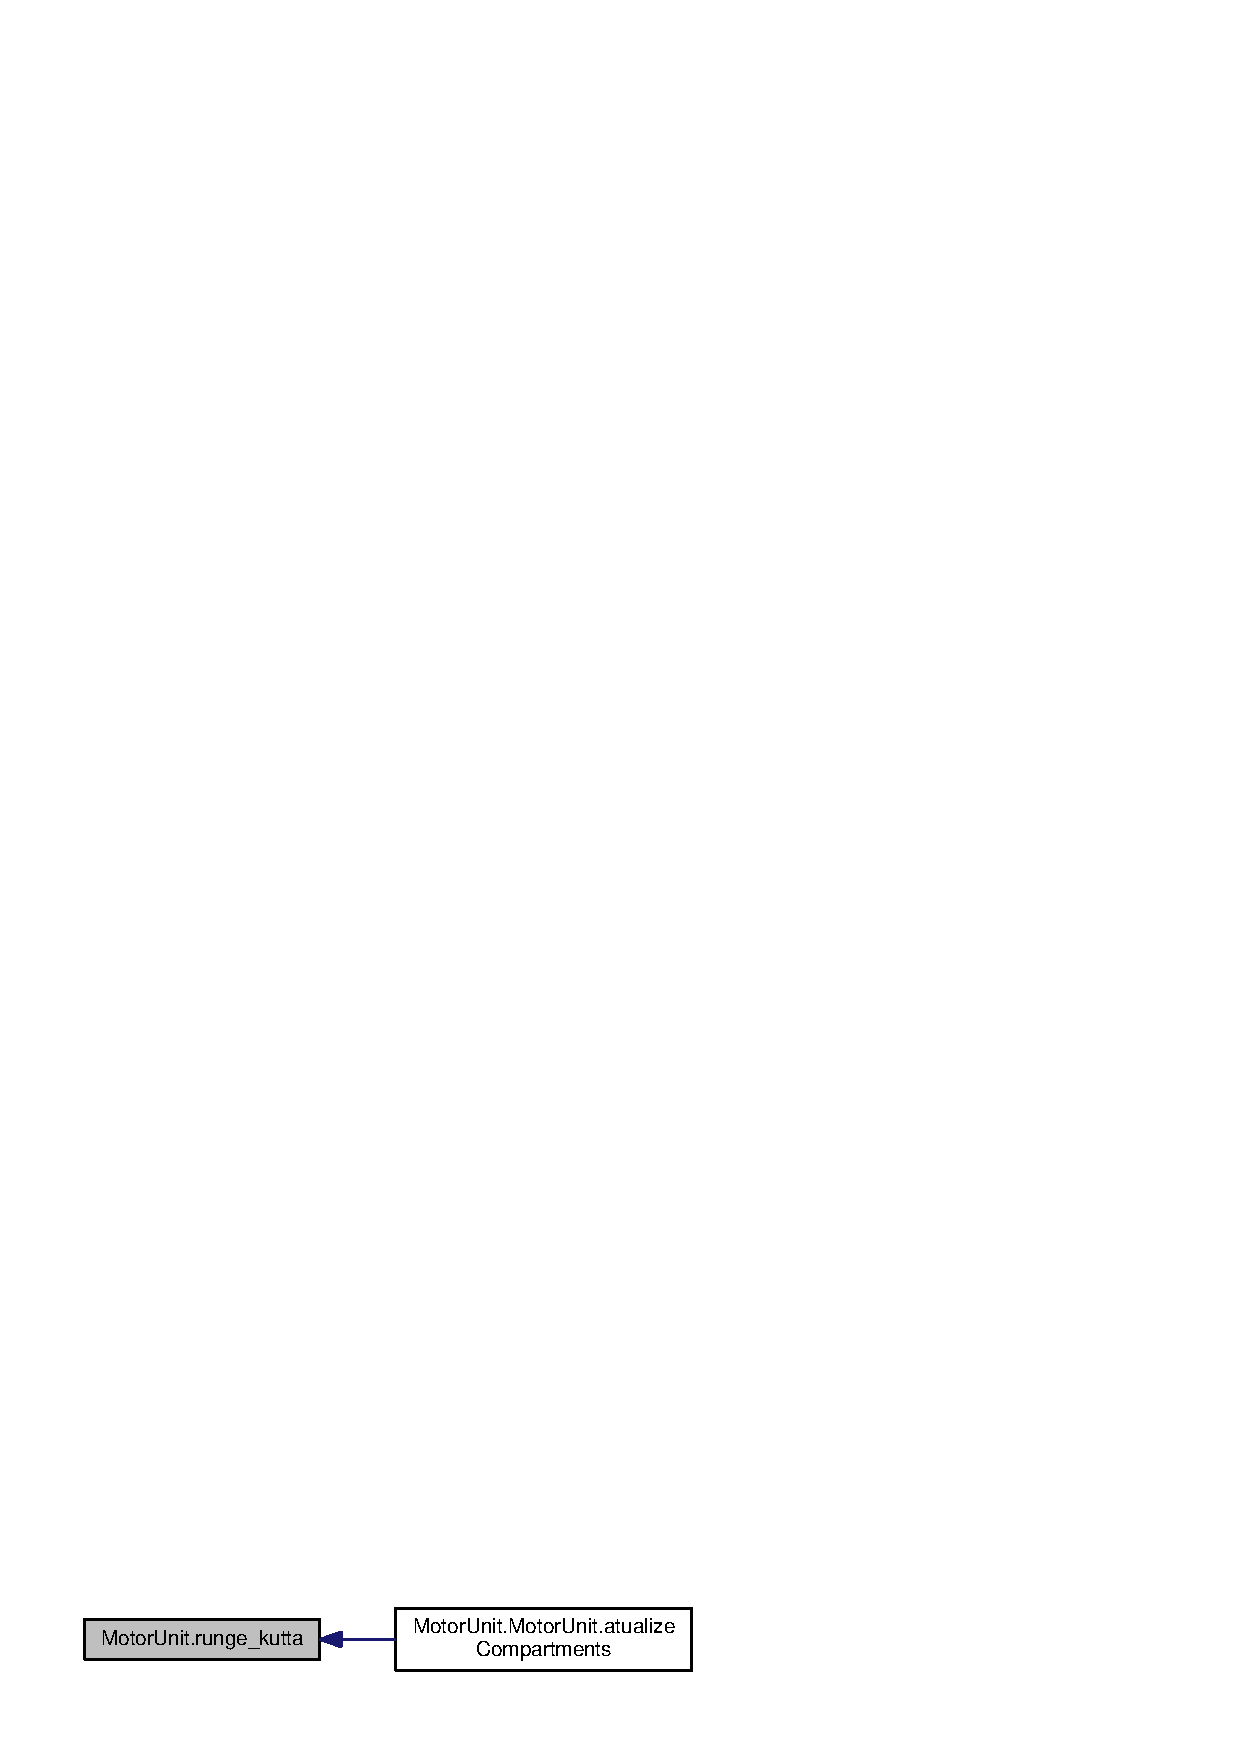
\includegraphics[width=350pt]{namespace_motor_unit_ad34c81597ff5e9cdcf53fd13e78d2d6c_icgraph}
\end{center}
\end{figure}



\hypertarget{namespace_motor_unit_pool}{\section{Motor\-Unit\-Pool Namespace Reference}
\label{namespace_motor_unit_pool}\index{Motor\-Unit\-Pool@{Motor\-Unit\-Pool}}
}
\subsection*{Classes}
\begin{DoxyCompactItemize}
\item 
class \hyperlink{class_motor_unit_pool_1_1_motor_unit_pool}{Motor\-Unit\-Pool}
\begin{DoxyCompactList}\small\item\em Class that implements a motor unit pool. \end{DoxyCompactList}\end{DoxyCompactItemize}
\subsection*{Functions}
\begin{DoxyCompactItemize}
\item 
def \hyperlink{namespace_motor_unit_pool_a3ed1b9ccd29068fac93964327dd54bf9}{twitch\-Saturation}
\begin{DoxyCompactList}\small\item\em Computes the muscle unit force after the nonlinear saturation. \end{DoxyCompactList}\end{DoxyCompactItemize}


\subsection{Function Documentation}
\hypertarget{namespace_motor_unit_pool_a3ed1b9ccd29068fac93964327dd54bf9}{\index{Motor\-Unit\-Pool@{Motor\-Unit\-Pool}!twitch\-Saturation@{twitch\-Saturation}}
\index{twitch\-Saturation@{twitch\-Saturation}!MotorUnitPool@{Motor\-Unit\-Pool}}
\subsubsection[{twitch\-Saturation}]{\setlength{\rightskip}{0pt plus 5cm}def Motor\-Unit\-Pool.\-twitch\-Saturation (
\begin{DoxyParamCaption}
\item[{}]{force, }
\item[{}]{b}
\end{DoxyParamCaption}
)}}\label{namespace_motor_unit_pool_a3ed1b9ccd29068fac93964327dd54bf9}


Computes the muscle unit force after the nonlinear saturation. 

\begin{equation} F_{sat} = \frac{1-e^{-b.force}}{1+e^{-b.force}} \end{equation}


\begin{DoxyItemize}
\item Inputs\-:
\begin{DoxyItemize}
\item {\bfseries force}\-: force before the saturation.
\item {\bfseries b}\-: saturation function parameter.
\end{DoxyItemize}
\item Outputs\-:
\begin{DoxyItemize}
\item Saturated force. 
\end{DoxyItemize}
\end{DoxyItemize}

Definition at line 31 of file Motor\-Unit\-Pool.\-py.



Here is the caller graph for this function\-:\nopagebreak
\begin{figure}[H]
\begin{center}
\leavevmode
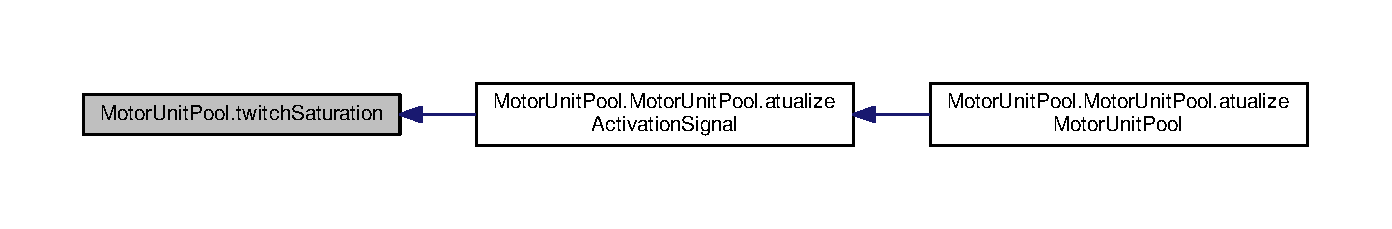
\includegraphics[width=350pt]{namespace_motor_unit_pool_a3ed1b9ccd29068fac93964327dd54bf9_icgraph}
\end{center}
\end{figure}



\hypertarget{namespace_neural_tract}{\section{Neural\-Tract Namespace Reference}
\label{namespace_neural_tract}\index{Neural\-Tract@{Neural\-Tract}}
}
\subsection*{Classes}
\begin{DoxyCompactItemize}
\item 
class \hyperlink{class_neural_tract_1_1_neural_tract}{Neural\-Tract}
\begin{DoxyCompactList}\small\item\em classdocs \end{DoxyCompactList}\end{DoxyCompactItemize}

\hypertarget{namespace_neural_tract_unit}{}\section{Neural\+Tract\+Unit Namespace Reference}
\label{namespace_neural_tract_unit}\index{Neural\+Tract\+Unit@{Neural\+Tract\+Unit}}
\subsection*{Classes}
\begin{DoxyCompactItemize}
\item 
class \hyperlink{class_neural_tract_unit_1_1_neural_tract_unit}{Neural\+Tract\+Unit}
\begin{DoxyCompactList}\small\item\em classdocs \end{DoxyCompactList}\end{DoxyCompactItemize}

\hypertarget{namespace_point_process_generator}{\section{Point\-Process\-Generator Namespace Reference}
\label{namespace_point_process_generator}\index{Point\-Process\-Generator@{Point\-Process\-Generator}}
}
\subsection*{Classes}
\begin{DoxyCompactItemize}
\item 
class \hyperlink{class_point_process_generator_1_1_point_process_generator}{Point\-Process\-Generator}
\begin{DoxyCompactList}\small\item\em classdocs \end{DoxyCompactList}\end{DoxyCompactItemize}
\subsection*{Functions}
\begin{DoxyCompactItemize}
\item 
def \hyperlink{namespace_point_process_generator_ad591b4c4f24356425c2958ea43647ddd}{gamma\-Point}
\end{DoxyCompactItemize}


\subsection{Function Documentation}
\hypertarget{namespace_point_process_generator_ad591b4c4f24356425c2958ea43647ddd}{\index{Point\-Process\-Generator@{Point\-Process\-Generator}!gamma\-Point@{gamma\-Point}}
\index{gamma\-Point@{gamma\-Point}!PointProcessGenerator@{Point\-Process\-Generator}}
\subsubsection[{gamma\-Point}]{\setlength{\rightskip}{0pt plus 5cm}def Point\-Process\-Generator.\-gamma\-Point (
\begin{DoxyParamCaption}
\item[{}]{Gamma\-Order}
\end{DoxyParamCaption}
)}}\label{namespace_point_process_generator_ad591b4c4f24356425c2958ea43647ddd}


Definition at line 15 of file Point\-Process\-Generator.\-py.


\hypertarget{namespace_pulse_conductance_state}{\section{Pulse\-Conductance\-State Namespace Reference}
\label{namespace_pulse_conductance_state}\index{Pulse\-Conductance\-State@{Pulse\-Conductance\-State}}
}
\subsection*{Classes}
\begin{DoxyCompactItemize}
\item 
class \hyperlink{class_pulse_conductance_state_1_1_pulse_conductance_state}{Pulse\-Conductance\-State}
\end{DoxyCompactItemize}
\subsection*{Functions}
\begin{DoxyCompactItemize}
\item 
def \hyperlink{namespace_pulse_conductance_state_ab354e94cc78939492454ad81c2e86223}{comp\-Val\-On}
\item 
def \hyperlink{namespace_pulse_conductance_state_a1cd804c6d3299a3ee17a4e96628e9ec7}{comp\-Val\-Off}
\end{DoxyCompactItemize}


\subsection{Function Documentation}
\hypertarget{namespace_pulse_conductance_state_a1cd804c6d3299a3ee17a4e96628e9ec7}{\index{Pulse\-Conductance\-State@{Pulse\-Conductance\-State}!comp\-Val\-Off@{comp\-Val\-Off}}
\index{comp\-Val\-Off@{comp\-Val\-Off}!PulseConductanceState@{Pulse\-Conductance\-State}}
\subsubsection[{comp\-Val\-Off}]{\setlength{\rightskip}{0pt plus 5cm}def Pulse\-Conductance\-State.\-comp\-Val\-Off (
\begin{DoxyParamCaption}
\item[{}]{v0, }
\item[{}]{alpha, }
\item[{}]{beta, }
\item[{}]{t, }
\item[{}]{t0}
\end{DoxyParamCaption}
)}}\label{namespace_pulse_conductance_state_a1cd804c6d3299a3ee17a4e96628e9ec7}


Definition at line 20 of file Pulse\-Conductance\-State.\-py.

\hypertarget{namespace_pulse_conductance_state_ab354e94cc78939492454ad81c2e86223}{\index{Pulse\-Conductance\-State@{Pulse\-Conductance\-State}!comp\-Val\-On@{comp\-Val\-On}}
\index{comp\-Val\-On@{comp\-Val\-On}!PulseConductanceState@{Pulse\-Conductance\-State}}
\subsubsection[{comp\-Val\-On}]{\setlength{\rightskip}{0pt plus 5cm}def Pulse\-Conductance\-State.\-comp\-Val\-On (
\begin{DoxyParamCaption}
\item[{}]{v0, }
\item[{}]{alpha, }
\item[{}]{beta, }
\item[{}]{t, }
\item[{}]{t0}
\end{DoxyParamCaption}
)}}\label{namespace_pulse_conductance_state_ab354e94cc78939492454ad81c2e86223}


Definition at line 15 of file Pulse\-Conductance\-State.\-py.


\hypertarget{namespacesimulation}{\section{simulation Namespace Reference}
\label{namespacesimulation}\index{simulation@{simulation}}
}
\subsection*{Functions}
\begin{DoxyCompactItemize}
\item 
def \hyperlink{namespacesimulation_a90ad3c33d4918e34f3ff6e6f69e9c2ec}{simulador}
\end{DoxyCompactItemize}


\subsection{Function Documentation}
\hypertarget{namespacesimulation_a90ad3c33d4918e34f3ff6e6f69e9c2ec}{\index{simulation@{simulation}!simulador@{simulador}}
\index{simulador@{simulador}!simulation@{simulation}}
\subsubsection[{simulador}]{\setlength{\rightskip}{0pt plus 5cm}def simulation.\-simulador (
\begin{DoxyParamCaption}
{}
\end{DoxyParamCaption}
)}}\label{namespacesimulation_a90ad3c33d4918e34f3ff6e6f69e9c2ec}


Definition at line 21 of file simulation.\-py.


\hypertarget{namespace_synapse}{}\section{Synapse Namespace Reference}
\label{namespace_synapse}\index{Synapse@{Synapse}}
\subsection*{Classes}
\begin{DoxyCompactItemize}
\item 
class \hyperlink{class_synapse_1_1_synapse}{Synapse}
\begin{DoxyCompactList}\small\item\em Implements the synapse model from Destexhe (1994) using the computational method from Lytton (1996). \end{DoxyCompactList}\end{DoxyCompactItemize}
\subsection*{Functions}
\begin{DoxyCompactItemize}
\item 
def \hyperlink{namespace_synapse_a400340da82be44ca7d665a8e04cd8974}{comp\+Synap\+Cond} (Gmax, Ron, Roff)
\begin{DoxyCompactList}\small\item\em Computes the synaptic conductance. \end{DoxyCompactList}\item 
def \hyperlink{namespace_synapse_a685fe07b10fd8ff53778983666836dea}{comp\+Ron} (Non, r\+Inf, Ron, t0, t, tau\+On)
\begin{DoxyCompactList}\small\item\em Computes the fraction of postsynaptic receptors that are bound to neurotransmitters of all the individual synapses that have neurotransmitters being released (during the pulse). \end{DoxyCompactList}\item 
def \hyperlink{namespace_synapse_a946e8e8437009fba80f7d7ead8d1eb57}{comp\+Roff} (Roff, t0, t, tau\+Off)
\begin{DoxyCompactList}\small\item\em Computes the fraction of postsynaptic receptors that are bound to neurotransmitters of all the individual synapses that do not have neurotransmitters being released (before and after the pulse). \end{DoxyCompactList}\item 
def \hyperlink{namespace_synapse_a86ce19e1d63e7071f6315234ee4cb6b6}{comp\+Ri\+Start} (ri, t, ti, t\+Peak, tau\+Off)
\begin{DoxyCompactList}\small\item\em Computes the fraction of bound postsynaptic receptors to neurotransmitters in individual synapses when the neurotransmitter begin (begin of the pulse). \end{DoxyCompactList}\item 
def \hyperlink{namespace_synapse_ad8ba0d5cb97f96cf8f68a75efc924488}{comp\+Ri\+Stop} (r\+Inf, ri, exp\+Finish)
\begin{DoxyCompactList}\small\item\em Computes the fraction of bound postsynaptic receptors to neurotransmitters in individual synapses when the neurotransmitter release stops (the pulse ends). \end{DoxyCompactList}\item 
def \hyperlink{namespace_synapse_a15925cbb893ee12094ad1861749e3240}{comp\+Ron\+Start} (Ron, ri, syn\+Contrib)
\begin{DoxyCompactList}\small\item\em Incorporates a new conductance to the set of conductances during a pulse. \end{DoxyCompactList}\item 
def \hyperlink{namespace_synapse_a695380d931b5beeed57d872bfddc423a}{comp\+Roff\+Start} (Roff, ri, syn\+Contrib)
\begin{DoxyCompactList}\small\item\em Incorporates a new conductance to the set of conductances that are not during a pulse. \end{DoxyCompactList}\item 
def \hyperlink{namespace_synapse_a3fb4510e3284ad84eb4d3d8c39112a94}{comp\+Ron\+Stop} (Ron, ri, syn\+Contrib)
\begin{DoxyCompactList}\small\item\em Removes a conductance from the set of conductances during a pulse. \end{DoxyCompactList}\item 
def \hyperlink{namespace_synapse_afd15218d4cf7a043cd35aa37f1593f6d}{comp\+Roff\+Stop} (Roff, ri, syn\+Contrib)
\begin{DoxyCompactList}\small\item\em Removes a conductance from the set of conductances that are not during a pulse. \end{DoxyCompactList}\item 
def \hyperlink{namespace_synapse_a8bf27e583af5778833e20c4468c6e71e}{comp\+Dynamic\+Gmax} (t, gmax, last\+Pulse, tau, dynamic\+Gmax, var)
\end{DoxyCompactItemize}


\subsection{Function Documentation}
\index{Synapse@{Synapse}!comp\+Dynamic\+Gmax@{comp\+Dynamic\+Gmax}}
\index{comp\+Dynamic\+Gmax@{comp\+Dynamic\+Gmax}!Synapse@{Synapse}}
\subsubsection[{\texorpdfstring{comp\+Dynamic\+Gmax(t, gmax, last\+Pulse, tau, dynamic\+Gmax, var)}{compDynamicGmax(t, gmax, lastPulse, tau, dynamicGmax, var)}}]{\setlength{\rightskip}{0pt plus 5cm}def Synapse.\+comp\+Dynamic\+Gmax (
\begin{DoxyParamCaption}
\item[{}]{t, }
\item[{}]{gmax, }
\item[{}]{last\+Pulse, }
\item[{}]{tau, }
\item[{}]{dynamic\+Gmax, }
\item[{}]{var}
\end{DoxyParamCaption}
)}\hypertarget{namespace_synapse_a8bf27e583af5778833e20c4468c6e71e}{}\label{namespace_synapse_a8bf27e583af5778833e20c4468c6e71e}


Definition at line 313 of file Synapse.\+py.

\index{Synapse@{Synapse}!comp\+Ri\+Start@{comp\+Ri\+Start}}
\index{comp\+Ri\+Start@{comp\+Ri\+Start}!Synapse@{Synapse}}
\subsubsection[{\texorpdfstring{comp\+Ri\+Start(ri, t, ti, t\+Peak, tau\+Off)}{compRiStart(ri, t, ti, tPeak, tauOff)}}]{\setlength{\rightskip}{0pt plus 5cm}def Synapse.\+comp\+Ri\+Start (
\begin{DoxyParamCaption}
\item[{}]{ri, }
\item[{}]{t, }
\item[{}]{ti, }
\item[{}]{t\+Peak, }
\item[{}]{tau\+Off}
\end{DoxyParamCaption}
)}\hypertarget{namespace_synapse_a86ce19e1d63e7071f6315234ee4cb6b6}{}\label{namespace_synapse_a86ce19e1d63e7071f6315234ee4cb6b6}


Computes the fraction of bound postsynaptic receptors to neurotransmitters in individual synapses when the neurotransmitter begin (begin of the pulse). 


\begin{DoxyItemize}
\item Inputs\+:
\begin{DoxyItemize}
\item {\bfseries ri}\+: the fraction of postsynaptic receptors that were bound to neurotransmitters at the last state change.
\item {\bfseries t}\+: current instant, in ms.
\item {\bfseries ti}\+: The instant that the last pulse began.
\item {\bfseries t\+Peak}\+: The duration of the pulse.
\item {\bfseries tau\+Off}\+: Time constant after a pulse, in ms.
\end{DoxyItemize}
\item Output\+:
\begin{DoxyItemize}
\item individual synapse state value.
\end{DoxyItemize}
\end{DoxyItemize}

It is computed by the following equation\+:

\begin{equation} r_{i_{newValue}} = r_{i_{oldValue}} \exp\left(\frac{t_i+T_{dur}-t}{\tau_{off}}\right) \end{equation} 

Definition at line 148 of file Synapse.\+py.

\index{Synapse@{Synapse}!comp\+Ri\+Stop@{comp\+Ri\+Stop}}
\index{comp\+Ri\+Stop@{comp\+Ri\+Stop}!Synapse@{Synapse}}
\subsubsection[{\texorpdfstring{comp\+Ri\+Stop(r\+Inf, ri, exp\+Finish)}{compRiStop(rInf, ri, expFinish)}}]{\setlength{\rightskip}{0pt plus 5cm}def Synapse.\+comp\+Ri\+Stop (
\begin{DoxyParamCaption}
\item[{}]{r\+Inf, }
\item[{}]{ri, }
\item[{}]{exp\+Finish}
\end{DoxyParamCaption}
)}\hypertarget{namespace_synapse_ad8ba0d5cb97f96cf8f68a75efc924488}{}\label{namespace_synapse_ad8ba0d5cb97f96cf8f68a75efc924488}


Computes the fraction of bound postsynaptic receptors to neurotransmitters in individual synapses when the neurotransmitter release stops (the pulse ends). 


\begin{DoxyItemize}
\item Inputs\+:
\begin{DoxyItemize}
\item {\bfseries r\+Inf}\+: the fraction of postsynaptic receptors that would be bound to neurotransmitters after an infinite amount of time with neurotransmitter being released.
\item {\bfseries ri}\+: the fraction of postsynaptic receptors that were bound to neurotransmitters at the last state change.
\item {\bfseries exp\+Finish}\+: Is the value of the exponential at the end of the pulse ( $\exp(T_{dur}/\tau_{on})$). It is is computed before for computational efficiency.
\end{DoxyItemize}
\item Output\+:
\begin{DoxyItemize}
\item individual synapse state value.
\end{DoxyItemize}
\end{DoxyItemize}

It is computed by the following equation\+:

\begin{equation} r_{i_{newValue}} = r_{\infty} + (r_{i_{oldValue}} - r_{\infty}) \exp\left(\frac{T_{dur}}{\tau_{on}}\right) \end{equation} 

Definition at line 180 of file Synapse.\+py.

\index{Synapse@{Synapse}!comp\+Roff@{comp\+Roff}}
\index{comp\+Roff@{comp\+Roff}!Synapse@{Synapse}}
\subsubsection[{\texorpdfstring{comp\+Roff(\+Roff, t0, t, tau\+Off)}{compRoff(Roff, t0, t, tauOff)}}]{\setlength{\rightskip}{0pt plus 5cm}def Synapse.\+comp\+Roff (
\begin{DoxyParamCaption}
\item[{}]{Roff, }
\item[{}]{t0, }
\item[{}]{t, }
\item[{}]{tau\+Off}
\end{DoxyParamCaption}
)}\hypertarget{namespace_synapse_a946e8e8437009fba80f7d7ead8d1eb57}{}\label{namespace_synapse_a946e8e8437009fba80f7d7ead8d1eb57}


Computes the fraction of postsynaptic receptors that are bound to neurotransmitters of all the individual synapses that do not have neurotransmitters being released (before and after the pulse). 


\begin{DoxyItemize}
\item Inputs\+:
\begin{DoxyItemize}
\item {\bfseries Roff}\+: sum of the fraction of postsynaptic receptors that are bound to neurotransmitters of all the individual synapses that do not have neurotransmitters being released (before and after the pulse).
\item {\bfseries t0}\+: instant that the last spike arrived to the compartment.
\item {\bfseries t}\+: current instant, in ms.
\item {\bfseries tau\+Off}\+: time constant after a pulse, in ms.
\end{DoxyItemize}
\item Output\+:
\begin{DoxyItemize}
\item The fraction of postsynaptic receptors that are bound to neurotransmitters of all the individual synapses that do not have neurotransmitters being released.
\end{DoxyItemize}
\end{DoxyItemize}

It is computed by the following formula\+:

\begin{equation} R_{off_{newValue}} = R_{off_{oldValue}}\exp\left(-\frac{t - t0}{\tau_{off}} \right) \end{equation} 

Definition at line 117 of file Synapse.\+py.

\index{Synapse@{Synapse}!comp\+Roff\+Start@{comp\+Roff\+Start}}
\index{comp\+Roff\+Start@{comp\+Roff\+Start}!Synapse@{Synapse}}
\subsubsection[{\texorpdfstring{comp\+Roff\+Start(\+Roff, ri, syn\+Contrib)}{compRoffStart(Roff, ri, synContrib)}}]{\setlength{\rightskip}{0pt plus 5cm}def Synapse.\+comp\+Roff\+Start (
\begin{DoxyParamCaption}
\item[{}]{Roff, }
\item[{}]{ri, }
\item[{}]{syn\+Contrib}
\end{DoxyParamCaption}
)}\hypertarget{namespace_synapse_a695380d931b5beeed57d872bfddc423a}{}\label{namespace_synapse_a695380d931b5beeed57d872bfddc423a}


Incorporates a new conductance to the set of conductances that are not during a pulse. 


\begin{DoxyItemize}
\item Inputs\+:
\begin{DoxyItemize}
\item {\bfseries Roff}\+: sum of the fraction of postsynaptic receptors that are bound to neurotransmitters of all the individual synapses that do not have neurotransmitters being released (before and after the pulse).
\item {\bfseries ri}\+: fraction of postsynaptic receptors that are bound to neurotransmitters of the individual synapses.
\item {\bfseries syn\+Contrib}\+: individual conductance constribution to the global synaptic conductance.
\end{DoxyItemize}
\item Output\+:
\begin{DoxyItemize}
\item The new value of the sum of the fraction of postsynaptic receptors that are bound to neurotransmitters of all the individual synapses that do not have neurotransmitters being released (before and after the pulse).
\end{DoxyItemize}
\end{DoxyItemize}

It is computed as\+:

\begin{equation} R_{off_{newValue}} = R_{off_{oldValue}} - r_iS_{indCont} \end{equation} 

Definition at line 244 of file Synapse.\+py.

\index{Synapse@{Synapse}!comp\+Roff\+Stop@{comp\+Roff\+Stop}}
\index{comp\+Roff\+Stop@{comp\+Roff\+Stop}!Synapse@{Synapse}}
\subsubsection[{\texorpdfstring{comp\+Roff\+Stop(\+Roff, ri, syn\+Contrib)}{compRoffStop(Roff, ri, synContrib)}}]{\setlength{\rightskip}{0pt plus 5cm}def Synapse.\+comp\+Roff\+Stop (
\begin{DoxyParamCaption}
\item[{}]{Roff, }
\item[{}]{ri, }
\item[{}]{syn\+Contrib}
\end{DoxyParamCaption}
)}\hypertarget{namespace_synapse_afd15218d4cf7a043cd35aa37f1593f6d}{}\label{namespace_synapse_afd15218d4cf7a043cd35aa37f1593f6d}


Removes a conductance from the set of conductances that are not during a pulse. 


\begin{DoxyItemize}
\item Inputs\+:
\begin{DoxyItemize}
\item {\bfseries Roff}\+: sum of the fraction of postsynaptic receptors that are bound to neurotransmitters of all the individual synapses that do not have neurotransmitters being released (before and after the pulse).
\item {\bfseries ri}\+: fraction of postsynaptic receptors that are bound to neurotransmitters of the individual synapses.
\item {\bfseries syn\+Contrib}\+: individual conductance constribution to the global synaptic conductance.
\end{DoxyItemize}
\item Output\+:
\begin{DoxyItemize}
\item The new value of the sum of the fraction of postsynaptic receptors that are bound to neurotransmitters of all the individual synapses that do not have neurotransmitters being released (before and after the pulse).
\end{DoxyItemize}
\end{DoxyItemize}

It is computed as\+:

\begin{equation} R_{off_{newValue}} = R_{off_{oldValue}} + r_iS_{indCont} \end{equation} 

Definition at line 309 of file Synapse.\+py.

\index{Synapse@{Synapse}!comp\+Ron@{comp\+Ron}}
\index{comp\+Ron@{comp\+Ron}!Synapse@{Synapse}}
\subsubsection[{\texorpdfstring{comp\+Ron(\+Non, r\+Inf, Ron, t0, t, tau\+On)}{compRon(Non, rInf, Ron, t0, t, tauOn)}}]{\setlength{\rightskip}{0pt plus 5cm}def Synapse.\+comp\+Ron (
\begin{DoxyParamCaption}
\item[{}]{Non, }
\item[{}]{r\+Inf, }
\item[{}]{Ron, }
\item[{}]{t0, }
\item[{}]{t, }
\item[{}]{tau\+On}
\end{DoxyParamCaption}
)}\hypertarget{namespace_synapse_a685fe07b10fd8ff53778983666836dea}{}\label{namespace_synapse_a685fe07b10fd8ff53778983666836dea}


Computes the fraction of postsynaptic receptors that are bound to neurotransmitters of all the individual synapses that have neurotransmitters being released (during the pulse). 


\begin{DoxyItemize}
\item Inputs\+:
\begin{DoxyItemize}
\item {\bfseries Non}\+: sum of the fractions of the individual conductances that are receiving neurotransmitter (during pulse) relative to the $G_{max}$ ( $N_{on}=\limits\sum_{i=1}g_{i_{on}}/G_{max}$).
\item {\bfseries r\+Inf}\+: the fraction of postsynaptic receptors that would be bound to neurotransmitters after an infinite amount of time with neurotransmitter being released.
\item {\bfseries Ron}\+: sum of the fraction of postsynaptic receptors that are bound to neurotransmitters of all the individual synapses that have neurotransmitters being released (during the pulse).
\item {\bfseries t0}\+: instant that the last spike arrived to the compartment.
\item {\bfseries t}\+: current instant, in ms.
\item {\bfseries tau\+On}\+: Time constant during a pulse, in ms. $\tau_{on}=\frac{1}{\alpha.T_{max} +\beta}$.
\end{DoxyItemize}
\item Outputs\+:
\begin{DoxyItemize}
\item The fraction of postsynaptic receptors that are bound to neurotransmitters of all the individual synapses that have neurotransmitters being released
\end{DoxyItemize}
\end{DoxyItemize}

It is computed by the following equation\+:

\begin{equation} R_{on_{newValue}} = N_{on}r_{\infty}\Bigg[1-\exp\left(-\frac{t-t_0}{\tau_{on}}\right)\Bigg] + R_{on_{oldValue}}\exp\left(-\frac{t-t_0}{\tau_{on}}\right) \end{equation} 

Definition at line 81 of file Synapse.\+py.

\index{Synapse@{Synapse}!comp\+Ron\+Start@{comp\+Ron\+Start}}
\index{comp\+Ron\+Start@{comp\+Ron\+Start}!Synapse@{Synapse}}
\subsubsection[{\texorpdfstring{comp\+Ron\+Start(\+Ron, ri, syn\+Contrib)}{compRonStart(Ron, ri, synContrib)}}]{\setlength{\rightskip}{0pt plus 5cm}def Synapse.\+comp\+Ron\+Start (
\begin{DoxyParamCaption}
\item[{}]{Ron, }
\item[{}]{ri, }
\item[{}]{syn\+Contrib}
\end{DoxyParamCaption}
)}\hypertarget{namespace_synapse_a15925cbb893ee12094ad1861749e3240}{}\label{namespace_synapse_a15925cbb893ee12094ad1861749e3240}


Incorporates a new conductance to the set of conductances during a pulse. 


\begin{DoxyItemize}
\item Inputs\+:
\begin{DoxyItemize}
\item {\bfseries Ron}\+: sum of the fraction of postsynaptic receptors that are bound to neurotransmitters of all the individual synapses that have neurotransmitters being released (during the pulse).
\item {\bfseries ri}\+: fraction of postsynaptic receptors that are bound to neurotransmitters of the individual synapses.
\item {\bfseries syn\+Contrib}\+: individual conductance constribution to the global synaptic conductance.
\end{DoxyItemize}
\item Output\+:
\begin{DoxyItemize}
\item The new value of the sum of the fraction of postsynaptic receptors that are bound to neurotransmitters of all the individual synapses that have neurotransmitters being released (during the pulse).
\end{DoxyItemize}
\end{DoxyItemize}

It is computed as\+:

\begin{equation} R_{on_{newValue}} = R_{on_{oldValue}} + r_iS_{indCont} \end{equation} 

Definition at line 211 of file Synapse.\+py.

\index{Synapse@{Synapse}!comp\+Ron\+Stop@{comp\+Ron\+Stop}}
\index{comp\+Ron\+Stop@{comp\+Ron\+Stop}!Synapse@{Synapse}}
\subsubsection[{\texorpdfstring{comp\+Ron\+Stop(\+Ron, ri, syn\+Contrib)}{compRonStop(Ron, ri, synContrib)}}]{\setlength{\rightskip}{0pt plus 5cm}def Synapse.\+comp\+Ron\+Stop (
\begin{DoxyParamCaption}
\item[{}]{Ron, }
\item[{}]{ri, }
\item[{}]{syn\+Contrib}
\end{DoxyParamCaption}
)}\hypertarget{namespace_synapse_a3fb4510e3284ad84eb4d3d8c39112a94}{}\label{namespace_synapse_a3fb4510e3284ad84eb4d3d8c39112a94}


Removes a conductance from the set of conductances during a pulse. 


\begin{DoxyItemize}
\item Inputs\+:
\begin{DoxyItemize}
\item {\bfseries Ron}\+: sum of the fraction of postsynaptic receptors that are bound to neurotransmitters of all the individual synapses that have neurotransmitters being released (during the pulse).
\item {\bfseries ri}\+: fraction of postsynaptic receptors that are bound to neurotransmitters of the individual synapses.
\item {\bfseries syn\+Contrib}\+: individual conductance constribution to the global synaptic conductance.
\end{DoxyItemize}
\item Output\+:
\begin{DoxyItemize}
\item The new value of the sum of the fraction of postsynaptic receptors that are bound to neurotransmitters of all the individual synapses that have neurotransmitters being released (during the pulse).
\end{DoxyItemize}
\end{DoxyItemize}

It is computed as\+:

\begin{equation} R_{on_{newValue}} = R_{on_{oldValue}} - r_iS_{indCont} \end{equation} 

Definition at line 275 of file Synapse.\+py.

\index{Synapse@{Synapse}!comp\+Synap\+Cond@{comp\+Synap\+Cond}}
\index{comp\+Synap\+Cond@{comp\+Synap\+Cond}!Synapse@{Synapse}}
\subsubsection[{\texorpdfstring{comp\+Synap\+Cond(\+Gmax, Ron, Roff)}{compSynapCond(Gmax, Ron, Roff)}}]{\setlength{\rightskip}{0pt plus 5cm}def Synapse.\+comp\+Synap\+Cond (
\begin{DoxyParamCaption}
\item[{}]{Gmax, }
\item[{}]{Ron, }
\item[{}]{Roff}
\end{DoxyParamCaption}
)}\hypertarget{namespace_synapse_a400340da82be44ca7d665a8e04cd8974}{}\label{namespace_synapse_a400340da82be44ca7d665a8e04cd8974}


Computes the synaptic conductance. 


\begin{DoxyItemize}
\item Input\+:
\begin{DoxyItemize}
\item {\bfseries Gmax}\+: the sum of individual conductances of all synapses in the compartment, in $\mu$S.
\item {\bfseries Ron}\+: sum of the fraction of postsynaptic receptors that are bound to neurotransmitters of all the individual synapses that have neurotransmitters being released (during the pulse).
\item {\bfseries Roff}\+: sum of the fraction of postsynaptic receptors that are bound to neurotransmitters of all the individual synapses that do not have neurotransmitters being released (before and after the pulse).
\end{DoxyItemize}
\item Output\+:
\begin{DoxyItemize}
\item the synaptic conductance of all synapses in the compartment, in $\mu$S.
\end{DoxyItemize}
\end{DoxyItemize}

It is computed by the following formula\+:

\begin{equation} G = G_{max}(R_{on} + R_{off}) \end{equation} where $G$ is the synaptic conductance of all synapses in the compartment. 

Definition at line 41 of file Synapse.\+py.


\hypertarget{namespace_synapses_factory}{\section{Synapses\-Factory Namespace Reference}
\label{namespace_synapses_factory}\index{Synapses\-Factory@{Synapses\-Factory}}
}
\subsection*{Classes}
\begin{DoxyCompactItemize}
\item 
class \hyperlink{class_synapses_factory_1_1_synapses_factory}{Synapses\-Factory}
\begin{DoxyCompactList}\small\item\em classdocs \end{DoxyCompactList}\end{DoxyCompactItemize}

\chapter{Class Documentation}
\hypertarget{class_axon_delay_1_1_axon_delay}{\section{Axon\-Delay.\-Axon\-Delay Class Reference}
\label{class_axon_delay_1_1_axon_delay}\index{Axon\-Delay.\-Axon\-Delay@{Axon\-Delay.\-Axon\-Delay}}
}


Class that implements a delay correspondent to the nerve.  


\subsection*{Public Member Functions}
\begin{DoxyCompactItemize}
\item 
def \hyperlink{class_axon_delay_1_1_axon_delay_ae4b6037beb2f833d82c5703bcb47ffb0}{\-\_\-\-\_\-init\-\_\-\-\_\-}
\begin{DoxyCompactList}\small\item\em Constructor. \end{DoxyCompactList}\item 
def \hyperlink{class_axon_delay_1_1_axon_delay_a49115bea963cde5e2c4317510d73cf7c}{add\-Terminal\-Spike}
\begin{DoxyCompactList}\small\item\em Indicates to the \hyperlink{class_axon_delay_1_1_axon_delay}{Axon\-Delay} object that a spike has occurred in the Terminal. \end{DoxyCompactList}\item 
def \hyperlink{class_axon_delay_1_1_axon_delay_a5483df94745af77bf54f707f9a05a0e0}{add\-Spinal\-Spike}
\begin{DoxyCompactList}\small\item\em Indicates to the \hyperlink{class_axon_delay_1_1_axon_delay}{Axon\-Delay} object that a spike has occurred in the soma. \end{DoxyCompactList}\end{DoxyCompactItemize}
\subsection*{Public Attributes}
\begin{DoxyCompactItemize}
\item 
\hyperlink{class_axon_delay_1_1_axon_delay_a5dbb9b5002d4b54bf347f48337bdb1c6}{index}
\begin{DoxyCompactList}\small\item\em Integer corresponding to the motor unit order in the pool, according to the Henneman's principle (size principle). \end{DoxyCompactList}\item 
\hyperlink{class_axon_delay_1_1_axon_delay_a08ab7285929002db2108179ea9f5d5dd}{length\-\_\-m}
\begin{DoxyCompactList}\small\item\em Length, in m, of the part of the nerve that is not modelled as a delay. \end{DoxyCompactList}\item 
\hyperlink{class_axon_delay_1_1_axon_delay_a59cc448f95b38b88b7103c3058e8c397}{velocity\-\_\-m\-\_\-s}
\begin{DoxyCompactList}\small\item\em Velocity of conduction, in m/s, of the part of the nerve that is not modelled as a delay. \end{DoxyCompactList}\item 
\hyperlink{class_axon_delay_1_1_axon_delay_a3f6bb8f38c4474806544d01fbe9c0361}{stimulus\-Positionto\-Terminal}
\begin{DoxyCompactList}\small\item\em Distance, in m, of the stimulus position to the terminal. \end{DoxyCompactList}\item 
\hyperlink{class_axon_delay_1_1_axon_delay_a81ea09febed911b8f5e4d56a5f434f8d}{latency\-Stimulus\-Spinal\-\_\-ms}
\begin{DoxyCompactList}\small\item\em time, in ms, that the signal takes to travel between the stimulus and the spinal cord. \end{DoxyCompactList}\item 
\hyperlink{class_axon_delay_1_1_axon_delay_aaa0b8daf2629cd7fa19d539fe2168d0f}{latency\-Spinal\-Terminal\-\_\-ms}
\begin{DoxyCompactList}\small\item\em time, in ms, that the signal takes to travel between the spinal cord and the terminal. \end{DoxyCompactList}\item 
\hyperlink{class_axon_delay_1_1_axon_delay_a88845b9926b97db88174ce088d5af5e0}{latency\-Stimulus\-Terminal\-\_\-ms}
\begin{DoxyCompactList}\small\item\em time, in ms, tat the signal takes to travel between the stimulus and the terminal. \end{DoxyCompactList}\item 
\hyperlink{class_axon_delay_1_1_axon_delay_aba392d8938766355063cf4bf3a87962d}{terminal\-Spike\-Train}
\begin{DoxyCompactList}\small\item\em Float with instant, in ms, of the last spike in the terminal. \end{DoxyCompactList}\end{DoxyCompactItemize}


\subsection{Detailed Description}
Class that implements a delay correspondent to the nerve. 

This class corresponds to the part of the axon that is modeled with no dynamics. Ideally this class would not exist and all the axon would be modelled in the motor unit or sensory class with the proper dynamics. 

Definition at line 16 of file Axon\-Delay.\-py.



\subsection{Constructor \& Destructor Documentation}
\hypertarget{class_axon_delay_1_1_axon_delay_ae4b6037beb2f833d82c5703bcb47ffb0}{\index{Axon\-Delay\-::\-Axon\-Delay@{Axon\-Delay\-::\-Axon\-Delay}!\-\_\-\-\_\-init\-\_\-\-\_\-@{\-\_\-\-\_\-init\-\_\-\-\_\-}}
\index{\-\_\-\-\_\-init\-\_\-\-\_\-@{\-\_\-\-\_\-init\-\_\-\-\_\-}!AxonDelay::AxonDelay@{Axon\-Delay\-::\-Axon\-Delay}}
\subsubsection[{\-\_\-\-\_\-init\-\_\-\-\_\-}]{\setlength{\rightskip}{0pt plus 5cm}def Axon\-Delay.\-Axon\-Delay.\-\_\-\-\_\-init\-\_\-\-\_\- (
\begin{DoxyParamCaption}
\item[{}]{self, }
\item[{}]{conf, }
\item[{}]{nerve, }
\item[{}]{pool, }
\item[{}]{index}
\end{DoxyParamCaption}
)}}\label{class_axon_delay_1_1_axon_delay_ae4b6037beb2f833d82c5703bcb47ffb0}


Constructor. 


\begin{DoxyItemize}
\item Inputs\-:
\begin{DoxyItemize}
\item {\bfseries conf}\-: \hyperlink{namespace_configuration}{Configuration} object with the simulation parameters.
\item {\bfseries nerve}\-: string with type of the nerve. It can be {\itshape P\-T\-N} (posterior tibial nerve) or {\itshape C\-P\-N} (common peroneal nerve).
\item {\bfseries pool}\-: string with Motor unit pool to which the motor unit belongs.
\item {\bfseries index}\-: integer corresponding to the motor unit order in the pool, according to the Henneman's principle (size principle). 
\end{DoxyItemize}
\end{DoxyItemize}

Definition at line 35 of file Axon\-Delay.\-py.



\subsection{Member Function Documentation}
\hypertarget{class_axon_delay_1_1_axon_delay_a5483df94745af77bf54f707f9a05a0e0}{\index{Axon\-Delay\-::\-Axon\-Delay@{Axon\-Delay\-::\-Axon\-Delay}!add\-Spinal\-Spike@{add\-Spinal\-Spike}}
\index{add\-Spinal\-Spike@{add\-Spinal\-Spike}!AxonDelay::AxonDelay@{Axon\-Delay\-::\-Axon\-Delay}}
\subsubsection[{add\-Spinal\-Spike}]{\setlength{\rightskip}{0pt plus 5cm}def Axon\-Delay.\-Axon\-Delay.\-add\-Spinal\-Spike (
\begin{DoxyParamCaption}
\item[{}]{self, }
\item[{}]{t}
\end{DoxyParamCaption}
)}}\label{class_axon_delay_1_1_axon_delay_a5483df94745af77bf54f707f9a05a0e0}


Indicates to the \hyperlink{class_axon_delay_1_1_axon_delay}{Axon\-Delay} object that a spike has occurred in the soma. 


\begin{DoxyItemize}
\item Inputs\-:
\begin{DoxyItemize}
\item {\bfseries t}\-: current instant, in ms. 
\end{DoxyItemize}
\end{DoxyItemize}

Definition at line 76 of file Axon\-Delay.\-py.



Here is the call graph for this function\-:\nopagebreak
\begin{figure}[H]
\begin{center}
\leavevmode
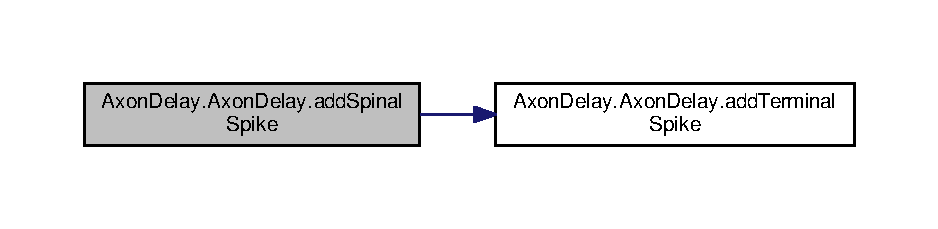
\includegraphics[width=350pt]{class_axon_delay_1_1_axon_delay_a5483df94745af77bf54f707f9a05a0e0_cgraph}
\end{center}
\end{figure}


\hypertarget{class_axon_delay_1_1_axon_delay_a49115bea963cde5e2c4317510d73cf7c}{\index{Axon\-Delay\-::\-Axon\-Delay@{Axon\-Delay\-::\-Axon\-Delay}!add\-Terminal\-Spike@{add\-Terminal\-Spike}}
\index{add\-Terminal\-Spike@{add\-Terminal\-Spike}!AxonDelay::AxonDelay@{Axon\-Delay\-::\-Axon\-Delay}}
\subsubsection[{add\-Terminal\-Spike}]{\setlength{\rightskip}{0pt plus 5cm}def Axon\-Delay.\-Axon\-Delay.\-add\-Terminal\-Spike (
\begin{DoxyParamCaption}
\item[{}]{self, }
\item[{}]{t}
\end{DoxyParamCaption}
)}}\label{class_axon_delay_1_1_axon_delay_a49115bea963cde5e2c4317510d73cf7c}


Indicates to the \hyperlink{class_axon_delay_1_1_axon_delay}{Axon\-Delay} object that a spike has occurred in the Terminal. 


\begin{DoxyItemize}
\item Inputs\-:
\begin{DoxyItemize}
\item {\bfseries t}\-: current instant, in ms. 
\end{DoxyItemize}
\end{DoxyItemize}

Definition at line 65 of file Axon\-Delay.\-py.



Here is the caller graph for this function\-:\nopagebreak
\begin{figure}[H]
\begin{center}
\leavevmode
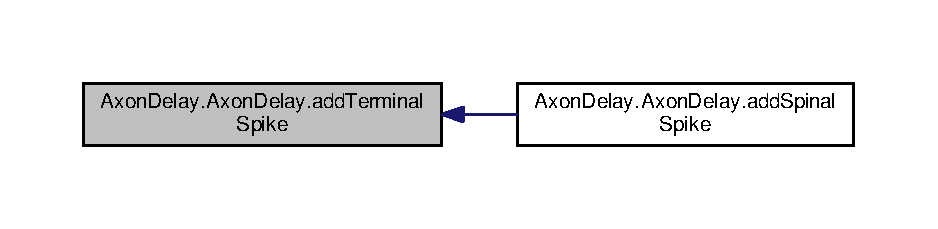
\includegraphics[width=350pt]{class_axon_delay_1_1_axon_delay_a49115bea963cde5e2c4317510d73cf7c_icgraph}
\end{center}
\end{figure}




\subsection{Member Data Documentation}
\hypertarget{class_axon_delay_1_1_axon_delay_a5dbb9b5002d4b54bf347f48337bdb1c6}{\index{Axon\-Delay\-::\-Axon\-Delay@{Axon\-Delay\-::\-Axon\-Delay}!index@{index}}
\index{index@{index}!AxonDelay::AxonDelay@{Axon\-Delay\-::\-Axon\-Delay}}
\subsubsection[{index}]{\setlength{\rightskip}{0pt plus 5cm}Axon\-Delay.\-Axon\-Delay.\-index}}\label{class_axon_delay_1_1_axon_delay_a5dbb9b5002d4b54bf347f48337bdb1c6}


Integer corresponding to the motor unit order in the pool, according to the Henneman's principle (size principle). 



Definition at line 39 of file Axon\-Delay.\-py.

\hypertarget{class_axon_delay_1_1_axon_delay_aaa0b8daf2629cd7fa19d539fe2168d0f}{\index{Axon\-Delay\-::\-Axon\-Delay@{Axon\-Delay\-::\-Axon\-Delay}!latency\-Spinal\-Terminal\-\_\-ms@{latency\-Spinal\-Terminal\-\_\-ms}}
\index{latency\-Spinal\-Terminal\-\_\-ms@{latency\-Spinal\-Terminal\-\_\-ms}!AxonDelay::AxonDelay@{Axon\-Delay\-::\-Axon\-Delay}}
\subsubsection[{latency\-Spinal\-Terminal\-\_\-ms}]{\setlength{\rightskip}{0pt plus 5cm}Axon\-Delay.\-Axon\-Delay.\-latency\-Spinal\-Terminal\-\_\-ms}}\label{class_axon_delay_1_1_axon_delay_aaa0b8daf2629cd7fa19d539fe2168d0f}


time, in ms, that the signal takes to travel between the spinal cord and the terminal. 



Definition at line 50 of file Axon\-Delay.\-py.

\hypertarget{class_axon_delay_1_1_axon_delay_a81ea09febed911b8f5e4d56a5f434f8d}{\index{Axon\-Delay\-::\-Axon\-Delay@{Axon\-Delay\-::\-Axon\-Delay}!latency\-Stimulus\-Spinal\-\_\-ms@{latency\-Stimulus\-Spinal\-\_\-ms}}
\index{latency\-Stimulus\-Spinal\-\_\-ms@{latency\-Stimulus\-Spinal\-\_\-ms}!AxonDelay::AxonDelay@{Axon\-Delay\-::\-Axon\-Delay}}
\subsubsection[{latency\-Stimulus\-Spinal\-\_\-ms}]{\setlength{\rightskip}{0pt plus 5cm}Axon\-Delay.\-Axon\-Delay.\-latency\-Stimulus\-Spinal\-\_\-ms}}\label{class_axon_delay_1_1_axon_delay_a81ea09febed911b8f5e4d56a5f434f8d}


time, in ms, that the signal takes to travel between the stimulus and the spinal cord. 



Definition at line 48 of file Axon\-Delay.\-py.

\hypertarget{class_axon_delay_1_1_axon_delay_a88845b9926b97db88174ce088d5af5e0}{\index{Axon\-Delay\-::\-Axon\-Delay@{Axon\-Delay\-::\-Axon\-Delay}!latency\-Stimulus\-Terminal\-\_\-ms@{latency\-Stimulus\-Terminal\-\_\-ms}}
\index{latency\-Stimulus\-Terminal\-\_\-ms@{latency\-Stimulus\-Terminal\-\_\-ms}!AxonDelay::AxonDelay@{Axon\-Delay\-::\-Axon\-Delay}}
\subsubsection[{latency\-Stimulus\-Terminal\-\_\-ms}]{\setlength{\rightskip}{0pt plus 5cm}Axon\-Delay.\-Axon\-Delay.\-latency\-Stimulus\-Terminal\-\_\-ms}}\label{class_axon_delay_1_1_axon_delay_a88845b9926b97db88174ce088d5af5e0}


time, in ms, tat the signal takes to travel between the stimulus and the terminal. 



Definition at line 52 of file Axon\-Delay.\-py.

\hypertarget{class_axon_delay_1_1_axon_delay_a08ab7285929002db2108179ea9f5d5dd}{\index{Axon\-Delay\-::\-Axon\-Delay@{Axon\-Delay\-::\-Axon\-Delay}!length\-\_\-m@{length\-\_\-m}}
\index{length\-\_\-m@{length\-\_\-m}!AxonDelay::AxonDelay@{Axon\-Delay\-::\-Axon\-Delay}}
\subsubsection[{length\-\_\-m}]{\setlength{\rightskip}{0pt plus 5cm}Axon\-Delay.\-Axon\-Delay.\-length\-\_\-m}}\label{class_axon_delay_1_1_axon_delay_a08ab7285929002db2108179ea9f5d5dd}


Length, in m, of the part of the nerve that is not modelled as a delay. 



Definition at line 42 of file Axon\-Delay.\-py.

\hypertarget{class_axon_delay_1_1_axon_delay_a3f6bb8f38c4474806544d01fbe9c0361}{\index{Axon\-Delay\-::\-Axon\-Delay@{Axon\-Delay\-::\-Axon\-Delay}!stimulus\-Positionto\-Terminal@{stimulus\-Positionto\-Terminal}}
\index{stimulus\-Positionto\-Terminal@{stimulus\-Positionto\-Terminal}!AxonDelay::AxonDelay@{Axon\-Delay\-::\-Axon\-Delay}}
\subsubsection[{stimulus\-Positionto\-Terminal}]{\setlength{\rightskip}{0pt plus 5cm}Axon\-Delay.\-Axon\-Delay.\-stimulus\-Positionto\-Terminal}}\label{class_axon_delay_1_1_axon_delay_a3f6bb8f38c4474806544d01fbe9c0361}


Distance, in m, of the stimulus position to the terminal. 



Definition at line 46 of file Axon\-Delay.\-py.

\hypertarget{class_axon_delay_1_1_axon_delay_aba392d8938766355063cf4bf3a87962d}{\index{Axon\-Delay\-::\-Axon\-Delay@{Axon\-Delay\-::\-Axon\-Delay}!terminal\-Spike\-Train@{terminal\-Spike\-Train}}
\index{terminal\-Spike\-Train@{terminal\-Spike\-Train}!AxonDelay::AxonDelay@{Axon\-Delay\-::\-Axon\-Delay}}
\subsubsection[{terminal\-Spike\-Train}]{\setlength{\rightskip}{0pt plus 5cm}Axon\-Delay.\-Axon\-Delay.\-terminal\-Spike\-Train}}\label{class_axon_delay_1_1_axon_delay_aba392d8938766355063cf4bf3a87962d}


Float with instant, in ms, of the last spike in the terminal. 



Definition at line 55 of file Axon\-Delay.\-py.

\hypertarget{class_axon_delay_1_1_axon_delay_a59cc448f95b38b88b7103c3058e8c397}{\index{Axon\-Delay\-::\-Axon\-Delay@{Axon\-Delay\-::\-Axon\-Delay}!velocity\-\_\-m\-\_\-s@{velocity\-\_\-m\-\_\-s}}
\index{velocity\-\_\-m\-\_\-s@{velocity\-\_\-m\-\_\-s}!AxonDelay::AxonDelay@{Axon\-Delay\-::\-Axon\-Delay}}
\subsubsection[{velocity\-\_\-m\-\_\-s}]{\setlength{\rightskip}{0pt plus 5cm}Axon\-Delay.\-Axon\-Delay.\-velocity\-\_\-m\-\_\-s}}\label{class_axon_delay_1_1_axon_delay_a59cc448f95b38b88b7103c3058e8c397}


Velocity of conduction, in m/s, of the part of the nerve that is not modelled as a delay. 



Definition at line 44 of file Axon\-Delay.\-py.



The documentation for this class was generated from the following file\-:\begin{DoxyCompactItemize}
\item 
\hyperlink{_axon_delay_8py}{Axon\-Delay.\-py}\end{DoxyCompactItemize}

\hypertarget{class_channel_conductance_1_1_channel_conductance}{\section{Channel\-Conductance.\-Channel\-Conductance Class Reference}
\label{class_channel_conductance_1_1_channel_conductance}\index{Channel\-Conductance.\-Channel\-Conductance@{Channel\-Conductance.\-Channel\-Conductance}}
}


Class that implements a model of the ionic Channels in a compartment.  


\subsection*{Public Member Functions}
\begin{DoxyCompactItemize}
\item 
def \hyperlink{class_channel_conductance_1_1_channel_conductance_adaaf5ea399963a716dc532a060964348}{\-\_\-\-\_\-init\-\_\-\-\_\-}
\begin{DoxyCompactList}\small\item\em Builds an ionic channel conductance. \end{DoxyCompactList}\item 
def \hyperlink{class_channel_conductance_1_1_channel_conductance_abde599b9096579b94d24295678f45b6d}{compute\-Current}
\begin{DoxyCompactList}\small\item\em Computes the current genrated by the ionic Channel. \end{DoxyCompactList}\item 
def \hyperlink{class_channel_conductance_1_1_channel_conductance_a956928953c88e1c03c113fc98ec42cc6}{comp\-Cond\-Kf}
\begin{DoxyCompactList}\small\item\em Computes the conductance of a Kf Channel. \end{DoxyCompactList}\item 
def \hyperlink{class_channel_conductance_1_1_channel_conductance_a19cc2a71f96187c7c647855d586cecaa}{comp\-Cond\-Ks}
\begin{DoxyCompactList}\small\item\em Computes the conductance of a Ks Channel. \end{DoxyCompactList}\item 
def \hyperlink{class_channel_conductance_1_1_channel_conductance_a26e6cf970cc7a8732f590dceb1d7c993}{comp\-Cond\-Na}
\begin{DoxyCompactList}\small\item\em Computes the conductance of a Na Channel. \end{DoxyCompactList}\end{DoxyCompactItemize}
\subsection*{Public Attributes}
\begin{DoxyCompactItemize}
\item 
\hyperlink{class_channel_conductance_1_1_channel_conductance_a7bf3e28aab2160014358cde589f2ec39}{kind}
\item 
\hyperlink{class_channel_conductance_1_1_channel_conductance_a628553cbc1efd93b30b0a15afd4417d9}{cond\-State}
\item 
\hyperlink{class_channel_conductance_1_1_channel_conductance_a654a73b6cd5853b509e7f7fba060572b}{Eq\-Pot\-\_\-m\-V}
\item 
\hyperlink{class_channel_conductance_1_1_channel_conductance_a80a0238a90b30b411c9381f682d0aeec}{gmax\-\_\-mu\-S}
\item 
\hyperlink{class_channel_conductance_1_1_channel_conductance_aa3c889bb4528c3abe7b69862cf87119d}{state\-Type}
\item 
\hyperlink{class_channel_conductance_1_1_channel_conductance_a0a91eec3fa2b1dfc66c6379943a5907f}{comp\-Cond}
\item 
\hyperlink{class_channel_conductance_1_1_channel_conductance_ae217799d13e5d225af048b7ba503fde1}{len\-States}
\end{DoxyCompactItemize}


\subsection{Detailed Description}
Class that implements a model of the ionic Channels in a compartment. 

Definition at line 16 of file Channel\-Conductance.\-py.



\subsection{Constructor \& Destructor Documentation}
\hypertarget{class_channel_conductance_1_1_channel_conductance_adaaf5ea399963a716dc532a060964348}{\index{Channel\-Conductance\-::\-Channel\-Conductance@{Channel\-Conductance\-::\-Channel\-Conductance}!\-\_\-\-\_\-init\-\_\-\-\_\-@{\-\_\-\-\_\-init\-\_\-\-\_\-}}
\index{\-\_\-\-\_\-init\-\_\-\-\_\-@{\-\_\-\-\_\-init\-\_\-\-\_\-}!ChannelConductance::ChannelConductance@{Channel\-Conductance\-::\-Channel\-Conductance}}
\subsubsection[{\-\_\-\-\_\-init\-\_\-\-\_\-}]{\setlength{\rightskip}{0pt plus 5cm}def Channel\-Conductance.\-Channel\-Conductance.\-\_\-\-\_\-init\-\_\-\-\_\- (
\begin{DoxyParamCaption}
\item[{}]{self, }
\item[{}]{kind, }
\item[{}]{conf, }
\item[{}]{comp\-Area, }
\item[{}]{pool, }
\item[{}]{index}
\end{DoxyParamCaption}
)}}\label{class_channel_conductance_1_1_channel_conductance_adaaf5ea399963a716dc532a060964348}


Builds an ionic channel conductance. 

Inputs\-: kind -\/ string with the type of the ionic channel (Na, Ks, Kf or Ca) conf -\/ instance of the \hyperlink{namespace_configuration}{Configuration} class (see \hyperlink{namespace_configuration}{Configuration} file) comp\-Area -\/ float with the area of the compartment that the Channel belongs, in cm2 pool -\/ the pool that this state belongs. index -\/ the index of the unit that this state belongs. 

Definition at line 30 of file Channel\-Conductance.\-py.



\subsection{Member Function Documentation}
\hypertarget{class_channel_conductance_1_1_channel_conductance_a956928953c88e1c03c113fc98ec42cc6}{\index{Channel\-Conductance\-::\-Channel\-Conductance@{Channel\-Conductance\-::\-Channel\-Conductance}!comp\-Cond\-Kf@{comp\-Cond\-Kf}}
\index{comp\-Cond\-Kf@{comp\-Cond\-Kf}!ChannelConductance::ChannelConductance@{Channel\-Conductance\-::\-Channel\-Conductance}}
\subsubsection[{comp\-Cond\-Kf}]{\setlength{\rightskip}{0pt plus 5cm}def Channel\-Conductance.\-Channel\-Conductance.\-comp\-Cond\-Kf (
\begin{DoxyParamCaption}
\item[{}]{self, }
\item[{}]{V\-\_\-m\-V}
\end{DoxyParamCaption}
)}}\label{class_channel_conductance_1_1_channel_conductance_a956928953c88e1c03c113fc98ec42cc6}


Computes the conductance of a Kf Channel. 

This function is assigned as self.\-comp\-Cond to a Kf Channel at the class constructor. \begin{DoxyVerb}    Input:
        V_mV - membrane potential of the compartment in mV

    Output:
        Conductance in muS\end{DoxyVerb}
 

Definition at line 90 of file Channel\-Conductance.\-py.

\hypertarget{class_channel_conductance_1_1_channel_conductance_a19cc2a71f96187c7c647855d586cecaa}{\index{Channel\-Conductance\-::\-Channel\-Conductance@{Channel\-Conductance\-::\-Channel\-Conductance}!comp\-Cond\-Ks@{comp\-Cond\-Ks}}
\index{comp\-Cond\-Ks@{comp\-Cond\-Ks}!ChannelConductance::ChannelConductance@{Channel\-Conductance\-::\-Channel\-Conductance}}
\subsubsection[{comp\-Cond\-Ks}]{\setlength{\rightskip}{0pt plus 5cm}def Channel\-Conductance.\-Channel\-Conductance.\-comp\-Cond\-Ks (
\begin{DoxyParamCaption}
\item[{}]{self, }
\item[{}]{V\-\_\-m\-V}
\end{DoxyParamCaption}
)}}\label{class_channel_conductance_1_1_channel_conductance_a19cc2a71f96187c7c647855d586cecaa}


Computes the conductance of a Ks Channel. 

This function is assigned as self.\-comp\-Cond to a Ks Channel at the class constructor. \begin{DoxyVerb}    Input:
        V_mV - membrane potential of the compartment in mV

    Output:
        Conductance in muS\end{DoxyVerb}
 

Definition at line 104 of file Channel\-Conductance.\-py.

\hypertarget{class_channel_conductance_1_1_channel_conductance_a26e6cf970cc7a8732f590dceb1d7c993}{\index{Channel\-Conductance\-::\-Channel\-Conductance@{Channel\-Conductance\-::\-Channel\-Conductance}!comp\-Cond\-Na@{comp\-Cond\-Na}}
\index{comp\-Cond\-Na@{comp\-Cond\-Na}!ChannelConductance::ChannelConductance@{Channel\-Conductance\-::\-Channel\-Conductance}}
\subsubsection[{comp\-Cond\-Na}]{\setlength{\rightskip}{0pt plus 5cm}def Channel\-Conductance.\-Channel\-Conductance.\-comp\-Cond\-Na (
\begin{DoxyParamCaption}
\item[{}]{self, }
\item[{}]{V\-\_\-m\-V}
\end{DoxyParamCaption}
)}}\label{class_channel_conductance_1_1_channel_conductance_a26e6cf970cc7a8732f590dceb1d7c993}


Computes the conductance of a Na Channel. 

This function is assigned as self.\-comp\-Cond to a Na Channel at the class constructor. \begin{DoxyVerb}    Input:
        V_mV - membrane potential of the compartment in mV

    Output:
        Conductance in muS\end{DoxyVerb}
 

Definition at line 118 of file Channel\-Conductance.\-py.

\hypertarget{class_channel_conductance_1_1_channel_conductance_abde599b9096579b94d24295678f45b6d}{\index{Channel\-Conductance\-::\-Channel\-Conductance@{Channel\-Conductance\-::\-Channel\-Conductance}!compute\-Current@{compute\-Current}}
\index{compute\-Current@{compute\-Current}!ChannelConductance::ChannelConductance@{Channel\-Conductance\-::\-Channel\-Conductance}}
\subsubsection[{compute\-Current}]{\setlength{\rightskip}{0pt plus 5cm}def Channel\-Conductance.\-Channel\-Conductance.\-compute\-Current (
\begin{DoxyParamCaption}
\item[{}]{self, }
\item[{}]{t, }
\item[{}]{V\-\_\-m\-V}
\end{DoxyParamCaption}
)}}\label{class_channel_conductance_1_1_channel_conductance_abde599b9096579b94d24295678f45b6d}


Computes the current genrated by the ionic Channel. 

Inputs\-: t -\/ instant in ms V\-\_\-m\-V -\/ membrane potential of the compartment in m\-V

Outputs\-: Ionic current in n\-A 

Definition at line 75 of file Channel\-Conductance.\-py.



\subsection{Member Data Documentation}
\hypertarget{class_channel_conductance_1_1_channel_conductance_a0a91eec3fa2b1dfc66c6379943a5907f}{\index{Channel\-Conductance\-::\-Channel\-Conductance@{Channel\-Conductance\-::\-Channel\-Conductance}!comp\-Cond@{comp\-Cond}}
\index{comp\-Cond@{comp\-Cond}!ChannelConductance::ChannelConductance@{Channel\-Conductance\-::\-Channel\-Conductance}}
\subsubsection[{comp\-Cond}]{\setlength{\rightskip}{0pt plus 5cm}Channel\-Conductance.\-Channel\-Conductance.\-comp\-Cond}}\label{class_channel_conductance_1_1_channel_conductance_a0a91eec3fa2b1dfc66c6379943a5907f}


Definition at line 44 of file Channel\-Conductance.\-py.

\hypertarget{class_channel_conductance_1_1_channel_conductance_a628553cbc1efd93b30b0a15afd4417d9}{\index{Channel\-Conductance\-::\-Channel\-Conductance@{Channel\-Conductance\-::\-Channel\-Conductance}!cond\-State@{cond\-State}}
\index{cond\-State@{cond\-State}!ChannelConductance::ChannelConductance@{Channel\-Conductance\-::\-Channel\-Conductance}}
\subsubsection[{cond\-State}]{\setlength{\rightskip}{0pt plus 5cm}Channel\-Conductance.\-Channel\-Conductance.\-cond\-State}}\label{class_channel_conductance_1_1_channel_conductance_a628553cbc1efd93b30b0a15afd4417d9}


Definition at line 32 of file Channel\-Conductance.\-py.

\hypertarget{class_channel_conductance_1_1_channel_conductance_a654a73b6cd5853b509e7f7fba060572b}{\index{Channel\-Conductance\-::\-Channel\-Conductance@{Channel\-Conductance\-::\-Channel\-Conductance}!Eq\-Pot\-\_\-m\-V@{Eq\-Pot\-\_\-m\-V}}
\index{Eq\-Pot\-\_\-m\-V@{Eq\-Pot\-\_\-m\-V}!ChannelConductance::ChannelConductance@{Channel\-Conductance\-::\-Channel\-Conductance}}
\subsubsection[{Eq\-Pot\-\_\-m\-V}]{\setlength{\rightskip}{0pt plus 5cm}Channel\-Conductance.\-Channel\-Conductance.\-Eq\-Pot\-\_\-m\-V}}\label{class_channel_conductance_1_1_channel_conductance_a654a73b6cd5853b509e7f7fba060572b}


Definition at line 34 of file Channel\-Conductance.\-py.

\hypertarget{class_channel_conductance_1_1_channel_conductance_a80a0238a90b30b411c9381f682d0aeec}{\index{Channel\-Conductance\-::\-Channel\-Conductance@{Channel\-Conductance\-::\-Channel\-Conductance}!gmax\-\_\-mu\-S@{gmax\-\_\-mu\-S}}
\index{gmax\-\_\-mu\-S@{gmax\-\_\-mu\-S}!ChannelConductance::ChannelConductance@{Channel\-Conductance\-::\-Channel\-Conductance}}
\subsubsection[{gmax\-\_\-mu\-S}]{\setlength{\rightskip}{0pt plus 5cm}Channel\-Conductance.\-Channel\-Conductance.\-gmax\-\_\-mu\-S}}\label{class_channel_conductance_1_1_channel_conductance_a80a0238a90b30b411c9381f682d0aeec}


Definition at line 35 of file Channel\-Conductance.\-py.

\hypertarget{class_channel_conductance_1_1_channel_conductance_a7bf3e28aab2160014358cde589f2ec39}{\index{Channel\-Conductance\-::\-Channel\-Conductance@{Channel\-Conductance\-::\-Channel\-Conductance}!kind@{kind}}
\index{kind@{kind}!ChannelConductance::ChannelConductance@{Channel\-Conductance\-::\-Channel\-Conductance}}
\subsubsection[{kind}]{\setlength{\rightskip}{0pt plus 5cm}Channel\-Conductance.\-Channel\-Conductance.\-kind}}\label{class_channel_conductance_1_1_channel_conductance_a7bf3e28aab2160014358cde589f2ec39}


Definition at line 31 of file Channel\-Conductance.\-py.

\hypertarget{class_channel_conductance_1_1_channel_conductance_ae217799d13e5d225af048b7ba503fde1}{\index{Channel\-Conductance\-::\-Channel\-Conductance@{Channel\-Conductance\-::\-Channel\-Conductance}!len\-States@{len\-States}}
\index{len\-States@{len\-States}!ChannelConductance::ChannelConductance@{Channel\-Conductance\-::\-Channel\-Conductance}}
\subsubsection[{len\-States}]{\setlength{\rightskip}{0pt plus 5cm}Channel\-Conductance.\-Channel\-Conductance.\-len\-States}}\label{class_channel_conductance_1_1_channel_conductance_ae217799d13e5d225af048b7ba503fde1}


Definition at line 58 of file Channel\-Conductance.\-py.

\hypertarget{class_channel_conductance_1_1_channel_conductance_aa3c889bb4528c3abe7b69862cf87119d}{\index{Channel\-Conductance\-::\-Channel\-Conductance@{Channel\-Conductance\-::\-Channel\-Conductance}!state\-Type@{state\-Type}}
\index{state\-Type@{state\-Type}!ChannelConductance::ChannelConductance@{Channel\-Conductance\-::\-Channel\-Conductance}}
\subsubsection[{state\-Type}]{\setlength{\rightskip}{0pt plus 5cm}Channel\-Conductance.\-Channel\-Conductance.\-state\-Type}}\label{class_channel_conductance_1_1_channel_conductance_aa3c889bb4528c3abe7b69862cf87119d}


Definition at line 37 of file Channel\-Conductance.\-py.



The documentation for this class was generated from the following file\-:\begin{DoxyCompactItemize}
\item 
\hyperlink{_channel_conductance_8py}{Channel\-Conductance.\-py}\end{DoxyCompactItemize}

\hypertarget{class_compartment_1_1_compartment}{\section{Compartment.\-Compartment Class Reference}
\label{class_compartment_1_1_compartment}\index{Compartment.\-Compartment@{Compartment.\-Compartment}}
}


classdocs  


\subsection*{Public Member Functions}
\begin{DoxyCompactItemize}
\item 
def \hyperlink{class_compartment_1_1_compartment_af6abb8e8999054b0f4d99c440dc06e42}{\-\_\-\-\_\-init\-\_\-\-\_\-}
\begin{DoxyCompactList}\small\item\em Constructor. \end{DoxyCompactList}\item 
def \hyperlink{class_compartment_1_1_compartment_ab10c374833a5c36df0552d40e64e45b9}{compute\-Current}
\end{DoxyCompactItemize}
\subsection*{Public Attributes}
\begin{DoxyCompactItemize}
\item 
\hyperlink{class_compartment_1_1_compartment_aa444563be9598d7cc54fd8d10ea6a04f}{Channels}
\item 
\hyperlink{class_compartment_1_1_compartment_ad42f32769afd94d1e7d7d54008efb6fa}{neuron\-Kind}
\item 
\hyperlink{class_compartment_1_1_compartment_a85d64ebf548276c873501d2dc3489ceb}{Synapses\-Out}
\item 
\hyperlink{class_compartment_1_1_compartment_abe41aff3bffed80f4b848bd14763d506}{Synapses\-In}
\item 
\hyperlink{class_compartment_1_1_compartment_a74f2266a2231c4a81cc680bc201f0ffd}{kind}
\item 
\hyperlink{class_compartment_1_1_compartment_a9402ef46ede52521ebbb9e9d2d68d631}{index}
\item 
\hyperlink{class_compartment_1_1_compartment_a8154742b0082eea301690e3566e477b6}{length\-\_\-mum}
\item 
\hyperlink{class_compartment_1_1_compartment_aacb7db7022f5d3534d17642d47281cbb}{diameter\-\_\-mum}
\item 
\hyperlink{class_compartment_1_1_compartment_a5d841c1a80dbaaf257dfc0a9cb763abc}{area\-\_\-cm2}
\item 
\hyperlink{class_compartment_1_1_compartment_aed6025b5335c2ce41d37c02fd3c1c042}{specif\-Res\-\_\-\-Ohmcm2}
\item 
\hyperlink{class_compartment_1_1_compartment_ac7d7462a45d4d623ed688c187c9184aa}{capacitance\-\_\-n\-F}
\item 
\hyperlink{class_compartment_1_1_compartment_a10d50da6a622982a6483c7cd78482bde}{g\-Leak}
\item 
\hyperlink{class_compartment_1_1_compartment_a0fa96147f76e7814f30610027ed425df}{number\-Channels}
\item 
\hyperlink{class_compartment_1_1_compartment_aed4deea8b0fc160f16ecb1ef39cacba4}{numberof\-Multi\-Synapses}
\end{DoxyCompactItemize}


\subsection{Detailed Description}
classdocs 

Definition at line 25 of file Compartment.\-py.



\subsection{Constructor \& Destructor Documentation}
\hypertarget{class_compartment_1_1_compartment_af6abb8e8999054b0f4d99c440dc06e42}{\index{Compartment\-::\-Compartment@{Compartment\-::\-Compartment}!\-\_\-\-\_\-init\-\_\-\-\_\-@{\-\_\-\-\_\-init\-\_\-\-\_\-}}
\index{\-\_\-\-\_\-init\-\_\-\-\_\-@{\-\_\-\-\_\-init\-\_\-\-\_\-}!Compartment::Compartment@{Compartment\-::\-Compartment}}
\subsubsection[{\-\_\-\-\_\-init\-\_\-\-\_\-}]{\setlength{\rightskip}{0pt plus 5cm}def Compartment.\-Compartment.\-\_\-\-\_\-init\-\_\-\-\_\- (
\begin{DoxyParamCaption}
\item[{}]{self, }
\item[{}]{kind, }
\item[{}]{conf, }
\item[{}]{pool, }
\item[{}]{index, }
\item[{}]{neuron\-Kind}
\end{DoxyParamCaption}
)}}\label{class_compartment_1_1_compartment_af6abb8e8999054b0f4d99c440dc06e42}


Constructor. 



Definition at line 32 of file Compartment.\-py.



\subsection{Member Function Documentation}
\hypertarget{class_compartment_1_1_compartment_ab10c374833a5c36df0552d40e64e45b9}{\index{Compartment\-::\-Compartment@{Compartment\-::\-Compartment}!compute\-Current@{compute\-Current}}
\index{compute\-Current@{compute\-Current}!Compartment::Compartment@{Compartment\-::\-Compartment}}
\subsubsection[{compute\-Current}]{\setlength{\rightskip}{0pt plus 5cm}def Compartment.\-Compartment.\-compute\-Current (
\begin{DoxyParamCaption}
\item[{}]{self, }
\item[{}]{t, }
\item[{}]{V\-\_\-m\-V}
\end{DoxyParamCaption}
)}}\label{class_compartment_1_1_compartment_ab10c374833a5c36df0552d40e64e45b9}


Definition at line 66 of file Compartment.\-py.



\subsection{Member Data Documentation}
\hypertarget{class_compartment_1_1_compartment_a5d841c1a80dbaaf257dfc0a9cb763abc}{\index{Compartment\-::\-Compartment@{Compartment\-::\-Compartment}!area\-\_\-cm2@{area\-\_\-cm2}}
\index{area\-\_\-cm2@{area\-\_\-cm2}!Compartment::Compartment@{Compartment\-::\-Compartment}}
\subsubsection[{area\-\_\-cm2}]{\setlength{\rightskip}{0pt plus 5cm}Compartment.\-Compartment.\-area\-\_\-cm2}}\label{class_compartment_1_1_compartment_a5d841c1a80dbaaf257dfc0a9cb763abc}


Definition at line 49 of file Compartment.\-py.

\hypertarget{class_compartment_1_1_compartment_ac7d7462a45d4d623ed688c187c9184aa}{\index{Compartment\-::\-Compartment@{Compartment\-::\-Compartment}!capacitance\-\_\-n\-F@{capacitance\-\_\-n\-F}}
\index{capacitance\-\_\-n\-F@{capacitance\-\_\-n\-F}!Compartment::Compartment@{Compartment\-::\-Compartment}}
\subsubsection[{capacitance\-\_\-n\-F}]{\setlength{\rightskip}{0pt plus 5cm}Compartment.\-Compartment.\-capacitance\-\_\-n\-F}}\label{class_compartment_1_1_compartment_ac7d7462a45d4d623ed688c187c9184aa}


Definition at line 51 of file Compartment.\-py.

\hypertarget{class_compartment_1_1_compartment_aa444563be9598d7cc54fd8d10ea6a04f}{\index{Compartment\-::\-Compartment@{Compartment\-::\-Compartment}!Channels@{Channels}}
\index{Channels@{Channels}!Compartment::Compartment@{Compartment\-::\-Compartment}}
\subsubsection[{Channels}]{\setlength{\rightskip}{0pt plus 5cm}Compartment.\-Compartment.\-Channels}}\label{class_compartment_1_1_compartment_aa444563be9598d7cc54fd8d10ea6a04f}


Definition at line 34 of file Compartment.\-py.

\hypertarget{class_compartment_1_1_compartment_aacb7db7022f5d3534d17642d47281cbb}{\index{Compartment\-::\-Compartment@{Compartment\-::\-Compartment}!diameter\-\_\-mum@{diameter\-\_\-mum}}
\index{diameter\-\_\-mum@{diameter\-\_\-mum}!Compartment::Compartment@{Compartment\-::\-Compartment}}
\subsubsection[{diameter\-\_\-mum}]{\setlength{\rightskip}{0pt plus 5cm}Compartment.\-Compartment.\-diameter\-\_\-mum}}\label{class_compartment_1_1_compartment_aacb7db7022f5d3534d17642d47281cbb}


Definition at line 48 of file Compartment.\-py.

\hypertarget{class_compartment_1_1_compartment_a10d50da6a622982a6483c7cd78482bde}{\index{Compartment\-::\-Compartment@{Compartment\-::\-Compartment}!g\-Leak@{g\-Leak}}
\index{g\-Leak@{g\-Leak}!Compartment::Compartment@{Compartment\-::\-Compartment}}
\subsubsection[{g\-Leak}]{\setlength{\rightskip}{0pt plus 5cm}Compartment.\-Compartment.\-g\-Leak}}\label{class_compartment_1_1_compartment_a10d50da6a622982a6483c7cd78482bde}


Definition at line 52 of file Compartment.\-py.

\hypertarget{class_compartment_1_1_compartment_a9402ef46ede52521ebbb9e9d2d68d631}{\index{Compartment\-::\-Compartment@{Compartment\-::\-Compartment}!index@{index}}
\index{index@{index}!Compartment::Compartment@{Compartment\-::\-Compartment}}
\subsubsection[{index}]{\setlength{\rightskip}{0pt plus 5cm}Compartment.\-Compartment.\-index}}\label{class_compartment_1_1_compartment_a9402ef46ede52521ebbb9e9d2d68d631}


Definition at line 45 of file Compartment.\-py.

\hypertarget{class_compartment_1_1_compartment_a74f2266a2231c4a81cc680bc201f0ffd}{\index{Compartment\-::\-Compartment@{Compartment\-::\-Compartment}!kind@{kind}}
\index{kind@{kind}!Compartment::Compartment@{Compartment\-::\-Compartment}}
\subsubsection[{kind}]{\setlength{\rightskip}{0pt plus 5cm}Compartment.\-Compartment.\-kind}}\label{class_compartment_1_1_compartment_a74f2266a2231c4a81cc680bc201f0ffd}


Definition at line 42 of file Compartment.\-py.

\hypertarget{class_compartment_1_1_compartment_a8154742b0082eea301690e3566e477b6}{\index{Compartment\-::\-Compartment@{Compartment\-::\-Compartment}!length\-\_\-mum@{length\-\_\-mum}}
\index{length\-\_\-mum@{length\-\_\-mum}!Compartment::Compartment@{Compartment\-::\-Compartment}}
\subsubsection[{length\-\_\-mum}]{\setlength{\rightskip}{0pt plus 5cm}Compartment.\-Compartment.\-length\-\_\-mum}}\label{class_compartment_1_1_compartment_a8154742b0082eea301690e3566e477b6}


Definition at line 47 of file Compartment.\-py.

\hypertarget{class_compartment_1_1_compartment_ad42f32769afd94d1e7d7d54008efb6fa}{\index{Compartment\-::\-Compartment@{Compartment\-::\-Compartment}!neuron\-Kind@{neuron\-Kind}}
\index{neuron\-Kind@{neuron\-Kind}!Compartment::Compartment@{Compartment\-::\-Compartment}}
\subsubsection[{neuron\-Kind}]{\setlength{\rightskip}{0pt plus 5cm}Compartment.\-Compartment.\-neuron\-Kind}}\label{class_compartment_1_1_compartment_ad42f32769afd94d1e7d7d54008efb6fa}


Definition at line 35 of file Compartment.\-py.

\hypertarget{class_compartment_1_1_compartment_a0fa96147f76e7814f30610027ed425df}{\index{Compartment\-::\-Compartment@{Compartment\-::\-Compartment}!number\-Channels@{number\-Channels}}
\index{number\-Channels@{number\-Channels}!Compartment::Compartment@{Compartment\-::\-Compartment}}
\subsubsection[{number\-Channels}]{\setlength{\rightskip}{0pt plus 5cm}Compartment.\-Compartment.\-number\-Channels}}\label{class_compartment_1_1_compartment_a0fa96147f76e7814f30610027ed425df}


Definition at line 62 of file Compartment.\-py.

\hypertarget{class_compartment_1_1_compartment_aed4deea8b0fc160f16ecb1ef39cacba4}{\index{Compartment\-::\-Compartment@{Compartment\-::\-Compartment}!numberof\-Multi\-Synapses@{numberof\-Multi\-Synapses}}
\index{numberof\-Multi\-Synapses@{numberof\-Multi\-Synapses}!Compartment::Compartment@{Compartment\-::\-Compartment}}
\subsubsection[{numberof\-Multi\-Synapses}]{\setlength{\rightskip}{0pt plus 5cm}Compartment.\-Compartment.\-numberof\-Multi\-Synapses}}\label{class_compartment_1_1_compartment_aed4deea8b0fc160f16ecb1ef39cacba4}


Definition at line 63 of file Compartment.\-py.

\hypertarget{class_compartment_1_1_compartment_aed6025b5335c2ce41d37c02fd3c1c042}{\index{Compartment\-::\-Compartment@{Compartment\-::\-Compartment}!specif\-Res\-\_\-\-Ohmcm2@{specif\-Res\-\_\-\-Ohmcm2}}
\index{specif\-Res\-\_\-\-Ohmcm2@{specif\-Res\-\_\-\-Ohmcm2}!Compartment::Compartment@{Compartment\-::\-Compartment}}
\subsubsection[{specif\-Res\-\_\-\-Ohmcm2}]{\setlength{\rightskip}{0pt plus 5cm}Compartment.\-Compartment.\-specif\-Res\-\_\-\-Ohmcm2}}\label{class_compartment_1_1_compartment_aed6025b5335c2ce41d37c02fd3c1c042}


Definition at line 50 of file Compartment.\-py.

\hypertarget{class_compartment_1_1_compartment_abe41aff3bffed80f4b848bd14763d506}{\index{Compartment\-::\-Compartment@{Compartment\-::\-Compartment}!Synapses\-In@{Synapses\-In}}
\index{Synapses\-In@{Synapses\-In}!Compartment::Compartment@{Compartment\-::\-Compartment}}
\subsubsection[{Synapses\-In}]{\setlength{\rightskip}{0pt plus 5cm}Compartment.\-Compartment.\-Synapses\-In}}\label{class_compartment_1_1_compartment_abe41aff3bffed80f4b848bd14763d506}


Definition at line 38 of file Compartment.\-py.

\hypertarget{class_compartment_1_1_compartment_a85d64ebf548276c873501d2dc3489ceb}{\index{Compartment\-::\-Compartment@{Compartment\-::\-Compartment}!Synapses\-Out@{Synapses\-Out}}
\index{Synapses\-Out@{Synapses\-Out}!Compartment::Compartment@{Compartment\-::\-Compartment}}
\subsubsection[{Synapses\-Out}]{\setlength{\rightskip}{0pt plus 5cm}Compartment.\-Compartment.\-Synapses\-Out}}\label{class_compartment_1_1_compartment_a85d64ebf548276c873501d2dc3489ceb}


Definition at line 36 of file Compartment.\-py.



The documentation for this class was generated from the following file\-:\begin{DoxyCompactItemize}
\item 
\hyperlink{_compartment_8py}{Compartment.\-py}\end{DoxyCompactItemize}

\hypertarget{class_configuration_1_1_configuration}{}\section{Configuration.\+Configuration Class Reference}
\label{class_configuration_1_1_configuration}\index{Configuration.\+Configuration@{Configuration.\+Configuration}}


Class that builds an object of \hyperlink{class_configuration_1_1_configuration}{Configuration}, based on a configuration file.  


\subsection*{Public Member Functions}
\begin{DoxyCompactItemize}
\item 
def \hyperlink{class_configuration_1_1_configuration_a2ba2e2fc97989c9d24632e4c403449c6}{\+\_\+\+\_\+init\+\_\+\+\_\+} (self, filename)
\begin{DoxyCompactList}\small\item\em Constructor. \end{DoxyCompactList}\item 
def \hyperlink{class_configuration_1_1_configuration_a31dc42dad64aef1518ca3fa14ea59625}{parameter\+Set} (self, param\+Tag, pool, index)
\begin{DoxyCompactList}\small\item\em Function that returns the value of wished parameter specified in the param\+Tag variable. \end{DoxyCompactList}\item 
def \hyperlink{class_configuration_1_1_configuration_a4fa34cff99386a55f1499f4dcdcd22be}{input\+Function\+Get} (self, function)
\begin{DoxyCompactList}\small\item\em Returns a numpy array with the values of the function for the whole simulation. \end{DoxyCompactList}\item 
def \hyperlink{class_configuration_1_1_configuration_ac2160d0341a793aa0fc1211757f08a73}{determine\+Synapses} (self, neural\+Source)
\begin{DoxyCompactList}\small\item\em Function used to determine all the synapses that a given pool makes. \end{DoxyCompactList}\end{DoxyCompactItemize}
\subsection*{Public Attributes}
\begin{DoxyCompactItemize}
\item 
\hyperlink{class_configuration_1_1_configuration_a2b8c2d210ef82ba5088de3c8c9a8725d}{conf\+Array}
\begin{DoxyCompactList}\small\item\em An array with all the simulation parameters. \end{DoxyCompactList}\item 
\hyperlink{class_configuration_1_1_configuration_a6379aaa6e54523ca81e3713d1846679b}{time\+Step\+\_\+ms}
\begin{DoxyCompactList}\small\item\em Time step of the numerical solution of the differential equation. \end{DoxyCompactList}\item 
\hyperlink{class_configuration_1_1_configuration_aea238884fe3daa1287aa069f35d4ad3e}{sim\+Duration\+\_\+ms}
\begin{DoxyCompactList}\small\item\em Total length of the simulation in ms. \end{DoxyCompactList}\item 
\hyperlink{class_configuration_1_1_configuration_a58f6e3bf5491f8fb229697fc3690aa12}{time\+Step\+By\+Two\+\_\+ms}
\begin{DoxyCompactList}\small\item\em The variable time\+Step divided by two, for computational efficiency. \end{DoxyCompactList}\item 
\hyperlink{class_configuration_1_1_configuration_aa49387a016f5d528136ab5812821cb99}{time\+Step\+By\+Six\+\_\+ms}
\begin{DoxyCompactList}\small\item\em The variable time\+Step divided by six, for computational efficiency. \end{DoxyCompactList}\end{DoxyCompactItemize}


\subsection{Detailed Description}
Class that builds an object of \hyperlink{class_configuration_1_1_configuration}{Configuration}, based on a configuration file. 

Definition at line 38 of file Configuration.\+py.



\subsection{Constructor \& Destructor Documentation}
\index{Configuration\+::\+Configuration@{Configuration\+::\+Configuration}!\+\_\+\+\_\+init\+\_\+\+\_\+@{\+\_\+\+\_\+init\+\_\+\+\_\+}}
\index{\+\_\+\+\_\+init\+\_\+\+\_\+@{\+\_\+\+\_\+init\+\_\+\+\_\+}!Configuration\+::\+Configuration@{Configuration\+::\+Configuration}}
\subsubsection[{\texorpdfstring{\+\_\+\+\_\+init\+\_\+\+\_\+(self, filename)}{__init__(self, filename)}}]{\setlength{\rightskip}{0pt plus 5cm}def Configuration.\+Configuration.\+\_\+\+\_\+init\+\_\+\+\_\+ (
\begin{DoxyParamCaption}
\item[{}]{self, }
\item[{}]{filename}
\end{DoxyParamCaption}
)}\hypertarget{class_configuration_1_1_configuration_a2ba2e2fc97989c9d24632e4c403449c6}{}\label{class_configuration_1_1_configuration_a2ba2e2fc97989c9d24632e4c403449c6}


Constructor. 

Builds the \hyperlink{class_configuration_1_1_configuration}{Configuration} object. A \hyperlink{class_configuration_1_1_configuration}{Configuration} object is responsible to set the variables that are used in the whole system, such as time\+Step and sim\+Duration.


\begin{DoxyItemize}
\item Inputs\+:
\begin{DoxyItemize}
\item {\bfseries filename}\+: name of the file with the parameter values. The extension of the file should be .rmto. 
\end{DoxyItemize}
\end{DoxyItemize}

Definition at line 52 of file Configuration.\+py.



\subsection{Member Function Documentation}
\index{Configuration\+::\+Configuration@{Configuration\+::\+Configuration}!determine\+Synapses@{determine\+Synapses}}
\index{determine\+Synapses@{determine\+Synapses}!Configuration\+::\+Configuration@{Configuration\+::\+Configuration}}
\subsubsection[{\texorpdfstring{determine\+Synapses(self, neural\+Source)}{determineSynapses(self, neuralSource)}}]{\setlength{\rightskip}{0pt plus 5cm}def Configuration.\+Configuration.\+determine\+Synapses (
\begin{DoxyParamCaption}
\item[{}]{self, }
\item[{}]{neural\+Source}
\end{DoxyParamCaption}
)}\hypertarget{class_configuration_1_1_configuration_ac2160d0341a793aa0fc1211757f08a73}{}\label{class_configuration_1_1_configuration_ac2160d0341a793aa0fc1211757f08a73}


Function used to determine all the synapses that a given pool makes. 

It is used in the \hyperlink{namespace_synapses_factory}{Synapses\+Factory} class.


\begin{DoxyItemize}
\item Inputs\+:
\begin{DoxyItemize}
\item {\bfseries neural\+Source} -\/ string with the pool name from which is desired to know what synapses it will make.
\end{DoxyItemize}
\item Outputs\+:
\begin{DoxyItemize}
\item array of strings with all the synapses target that the neural\+Source will make. 
\end{DoxyItemize}
\end{DoxyItemize}

Definition at line 164 of file Configuration.\+py.

\index{Configuration\+::\+Configuration@{Configuration\+::\+Configuration}!input\+Function\+Get@{input\+Function\+Get}}
\index{input\+Function\+Get@{input\+Function\+Get}!Configuration\+::\+Configuration@{Configuration\+::\+Configuration}}
\subsubsection[{\texorpdfstring{input\+Function\+Get(self, function)}{inputFunctionGet(self, function)}}]{\setlength{\rightskip}{0pt plus 5cm}def Configuration.\+Configuration.\+input\+Function\+Get (
\begin{DoxyParamCaption}
\item[{}]{self, }
\item[{}]{function}
\end{DoxyParamCaption}
)}\hypertarget{class_configuration_1_1_configuration_a4fa34cff99386a55f1499f4dcdcd22be}{}\label{class_configuration_1_1_configuration_a4fa34cff99386a55f1499f4dcdcd22be}


Returns a numpy array with the values of the function for the whole simulation. 

It is used to obtain before the simulation run all the values of the inputs.


\begin{DoxyItemize}
\item Inputs\+:
\begin{DoxyItemize}
\item {\bfseries function}\+: function from which is desired to obtain its values during the simulation duration.
\end{DoxyItemize}
\item Output\+:
\begin{DoxyItemize}
\item narray with the function values for each instant. 
\end{DoxyItemize}
\end{DoxyItemize}

Definition at line 148 of file Configuration.\+py.

\index{Configuration\+::\+Configuration@{Configuration\+::\+Configuration}!parameter\+Set@{parameter\+Set}}
\index{parameter\+Set@{parameter\+Set}!Configuration\+::\+Configuration@{Configuration\+::\+Configuration}}
\subsubsection[{\texorpdfstring{parameter\+Set(self, param\+Tag, pool, index)}{parameterSet(self, paramTag, pool, index)}}]{\setlength{\rightskip}{0pt plus 5cm}def Configuration.\+Configuration.\+parameter\+Set (
\begin{DoxyParamCaption}
\item[{}]{self, }
\item[{}]{param\+Tag, }
\item[{}]{pool, }
\item[{}]{index}
\end{DoxyParamCaption}
)}\hypertarget{class_configuration_1_1_configuration_a31dc42dad64aef1518ca3fa14ea59625}{}\label{class_configuration_1_1_configuration_a31dc42dad64aef1518ca3fa14ea59625}


Function that returns the value of wished parameter specified in the param\+Tag variable. 

In the case of min/max parameters, the value returned is the specific to the index of the unit that called the function.


\begin{DoxyItemize}
\item Inputs\+:
\begin{DoxyItemize}
\item {\bfseries param\+Tag}\+: string with the name of the wished parameter as in the first column of the rmto file.
\item {\bfseries pool}\+: pool from which the unit that will receive the parameter value belongs. For example S\+OL. It is used only in the parameters that have a range.
\item {\bfseries index}\+: index of the unit. It is is an integer.
\end{DoxyItemize}
\item Outputs\+:
\begin{DoxyItemize}
\item required parameter value 
\end{DoxyItemize}
\end{DoxyItemize}

Definition at line 92 of file Configuration.\+py.



\subsection{Member Data Documentation}
\index{Configuration\+::\+Configuration@{Configuration\+::\+Configuration}!conf\+Array@{conf\+Array}}
\index{conf\+Array@{conf\+Array}!Configuration\+::\+Configuration@{Configuration\+::\+Configuration}}
\subsubsection[{\texorpdfstring{conf\+Array}{confArray}}]{\setlength{\rightskip}{0pt plus 5cm}Configuration.\+Configuration.\+conf\+Array}\hypertarget{class_configuration_1_1_configuration_a2b8c2d210ef82ba5088de3c8c9a8725d}{}\label{class_configuration_1_1_configuration_a2b8c2d210ef82ba5088de3c8c9a8725d}


An array with all the simulation parameters. 



Definition at line 55 of file Configuration.\+py.

\index{Configuration\+::\+Configuration@{Configuration\+::\+Configuration}!sim\+Duration\+\_\+ms@{sim\+Duration\+\_\+ms}}
\index{sim\+Duration\+\_\+ms@{sim\+Duration\+\_\+ms}!Configuration\+::\+Configuration@{Configuration\+::\+Configuration}}
\subsubsection[{\texorpdfstring{sim\+Duration\+\_\+ms}{simDuration_ms}}]{\setlength{\rightskip}{0pt plus 5cm}Configuration.\+Configuration.\+sim\+Duration\+\_\+ms}\hypertarget{class_configuration_1_1_configuration_aea238884fe3daa1287aa069f35d4ad3e}{}\label{class_configuration_1_1_configuration_aea238884fe3daa1287aa069f35d4ad3e}


Total length of the simulation in ms. 



Definition at line 65 of file Configuration.\+py.

\index{Configuration\+::\+Configuration@{Configuration\+::\+Configuration}!time\+Step\+\_\+ms@{time\+Step\+\_\+ms}}
\index{time\+Step\+\_\+ms@{time\+Step\+\_\+ms}!Configuration\+::\+Configuration@{Configuration\+::\+Configuration}}
\subsubsection[{\texorpdfstring{time\+Step\+\_\+ms}{timeStep_ms}}]{\setlength{\rightskip}{0pt plus 5cm}Configuration.\+Configuration.\+time\+Step\+\_\+ms}\hypertarget{class_configuration_1_1_configuration_a6379aaa6e54523ca81e3713d1846679b}{}\label{class_configuration_1_1_configuration_a6379aaa6e54523ca81e3713d1846679b}


Time step of the numerical solution of the differential equation. 



Definition at line 62 of file Configuration.\+py.

\index{Configuration\+::\+Configuration@{Configuration\+::\+Configuration}!time\+Step\+By\+Six\+\_\+ms@{time\+Step\+By\+Six\+\_\+ms}}
\index{time\+Step\+By\+Six\+\_\+ms@{time\+Step\+By\+Six\+\_\+ms}!Configuration\+::\+Configuration@{Configuration\+::\+Configuration}}
\subsubsection[{\texorpdfstring{time\+Step\+By\+Six\+\_\+ms}{timeStepBySix_ms}}]{\setlength{\rightskip}{0pt plus 5cm}Configuration.\+Configuration.\+time\+Step\+By\+Six\+\_\+ms}\hypertarget{class_configuration_1_1_configuration_aa49387a016f5d528136ab5812821cb99}{}\label{class_configuration_1_1_configuration_aa49387a016f5d528136ab5812821cb99}


The variable time\+Step divided by six, for computational efficiency. 



Definition at line 69 of file Configuration.\+py.

\index{Configuration\+::\+Configuration@{Configuration\+::\+Configuration}!time\+Step\+By\+Two\+\_\+ms@{time\+Step\+By\+Two\+\_\+ms}}
\index{time\+Step\+By\+Two\+\_\+ms@{time\+Step\+By\+Two\+\_\+ms}!Configuration\+::\+Configuration@{Configuration\+::\+Configuration}}
\subsubsection[{\texorpdfstring{time\+Step\+By\+Two\+\_\+ms}{timeStepByTwo_ms}}]{\setlength{\rightskip}{0pt plus 5cm}Configuration.\+Configuration.\+time\+Step\+By\+Two\+\_\+ms}\hypertarget{class_configuration_1_1_configuration_a58f6e3bf5491f8fb229697fc3690aa12}{}\label{class_configuration_1_1_configuration_a58f6e3bf5491f8fb229697fc3690aa12}


The variable time\+Step divided by two, for computational efficiency. 



Definition at line 67 of file Configuration.\+py.



The documentation for this class was generated from the following file\+:\begin{DoxyCompactItemize}
\item 
\hyperlink{_configuration_8py}{Configuration.\+py}\end{DoxyCompactItemize}

\hypertarget{class_motor_unit_1_1_motor_unit}{}\section{Motor\+Unit.\+Motor\+Unit Class Reference}
\label{class_motor_unit_1_1_motor_unit}\index{Motor\+Unit.\+Motor\+Unit@{Motor\+Unit.\+Motor\+Unit}}


Class that implements a motor unit model.  


\subsection*{Public Member Functions}
\begin{DoxyCompactItemize}
\item 
def \hyperlink{class_motor_unit_1_1_motor_unit_ac5228576ec1287f06debf92067c7402b}{\+\_\+\+\_\+init\+\_\+\+\_\+} (self, \hyperlink{class_motor_unit_1_1_motor_unit_a10539f5129881188923f3a3a164d2cba}{conf}, pool, \hyperlink{class_motor_unit_1_1_motor_unit_a4f3205a9273aabb92d425992d91a1848}{index}, \hyperlink{class_motor_unit_1_1_motor_unit_a08ed5171ba46e0b1ea5bc7d08296c612}{kind})
\begin{DoxyCompactList}\small\item\em Constructor. \end{DoxyCompactList}\item 
def \hyperlink{class_motor_unit_1_1_motor_unit_ab57693c2f49518b08639456595e92d87}{atualize\+Motor\+Unit} (self, t)
\begin{DoxyCompactList}\small\item\em Atualize the dynamical and nondynamical (delay) parts of the motor unit. \end{DoxyCompactList}\item 
def \hyperlink{class_motor_unit_1_1_motor_unit_a666fa3bb4b8fb00f1217387a5ede5b7b}{atualize\+Compartments} (self, t)
\begin{DoxyCompactList}\small\item\em Atualize all neural compartments. \end{DoxyCompactList}\item 
def \hyperlink{class_motor_unit_1_1_motor_unit_adf30fdef09ac21cfc2a261b762a7f618}{d\+Vdt} (self, t, V)
\begin{DoxyCompactList}\small\item\em Compute the potential derivative of all compartments of the motor unit. \end{DoxyCompactList}\item 
def \hyperlink{class_motor_unit_1_1_motor_unit_a6d597c703b3b469fbec7843a0f97c534}{add\+Soma\+Spike} (self, t)
\begin{DoxyCompactList}\small\item\em When the soma potential is above the threshold a spike is added tom the soma. \end{DoxyCompactList}\item 
def \hyperlink{class_motor_unit_1_1_motor_unit_a0aa5e024003845e3f48bc0e618068edc}{atualize\+Delay} (self, t)
\begin{DoxyCompactList}\small\item\em Atualize the terminal spike train, by considering the Delay of the nerve. \end{DoxyCompactList}\item 
def \hyperlink{class_motor_unit_1_1_motor_unit_ac3d3e69bf0b75eef81a015005052f5d3}{transmit\+Spikes} (self, t)
\end{DoxyCompactItemize}
\subsection*{Public Attributes}
\begin{DoxyCompactItemize}
\item 
\hyperlink{class_motor_unit_1_1_motor_unit_a10539f5129881188923f3a3a164d2cba}{conf}
\begin{DoxyCompactList}\small\item\em \hyperlink{namespace_configuration}{Configuration} object with the simulation parameters. \end{DoxyCompactList}\item 
\hyperlink{class_motor_unit_1_1_motor_unit_a08ed5171ba46e0b1ea5bc7d08296c612}{kind}
\begin{DoxyCompactList}\small\item\em String with the type of the motor unit. \end{DoxyCompactList}\item 
\hyperlink{class_motor_unit_1_1_motor_unit_abca82ec2c7312bb475989bb45e82ca28}{t\+Soma\+Spike}
\begin{DoxyCompactList}\small\item\em The instant of the last spike of the Motor unit at the Soma compartment. \end{DoxyCompactList}\item 
\hyperlink{class_motor_unit_1_1_motor_unit_a8c86d98daa6c509e226ab165fa92515f}{soma\+Spike\+Train}
\begin{DoxyCompactList}\small\item\em Vector with the instants of spikes at the soma. \end{DoxyCompactList}\item 
\hyperlink{class_motor_unit_1_1_motor_unit_a4f3205a9273aabb92d425992d91a1848}{index}
\begin{DoxyCompactList}\small\item\em Integer corresponding to the motor unit order in the pool, according to the Henneman\textquotesingle{}s principle (size principle). \end{DoxyCompactList}\item 
\hyperlink{class_motor_unit_1_1_motor_unit_a6d4da7327031b3cb9c7041a4a790e524}{compartment}
\begin{DoxyCompactList}\small\item\em Vector of \hyperlink{namespace_compartment}{Compartment} of the Motor Unit. \end{DoxyCompactList}\item 
\hyperlink{class_motor_unit_1_1_motor_unit_affbd0b90f1dce6a0f929775e54f8c212}{threshold\+\_\+mV}
\begin{DoxyCompactList}\small\item\em Value of the membrane potential, in mV, that is considered a spike. \end{DoxyCompactList}\item 
\hyperlink{class_motor_unit_1_1_motor_unit_a9b1938bcbaa8c89ef47e0b915ab4cd39}{position\+\_\+mm}
\begin{DoxyCompactList}\small\item\em Anatomical position of the neuron, in mm. \end{DoxyCompactList}\item 
\hyperlink{class_motor_unit_1_1_motor_unit_afe7281fb12c41102980b6b48d5a49713}{comp\+Number}
\begin{DoxyCompactList}\small\item\em Number of compartments. \end{DoxyCompactList}\item 
\hyperlink{class_motor_unit_1_1_motor_unit_aa8968f89250895ae2ae572e9106709f2}{v\+\_\+mV}
\begin{DoxyCompactList}\small\item\em Vector with membrane potential,in mV, of all compartments. \end{DoxyCompactList}\item 
\hyperlink{class_motor_unit_1_1_motor_unit_a0cf2afb5bd12374db56b9d9a5a1671e6}{capacitance\+Inv}
\begin{DoxyCompactList}\small\item\em Vector with the inverse of the capacitance of all compartments. \end{DoxyCompactList}\item 
\hyperlink{class_motor_unit_1_1_motor_unit_a0541858216e7d01582312f9a7a99d595}{i\+Ionic}
\begin{DoxyCompactList}\small\item\em Vector with current, in nA, of each compartment coming from other elements of the model. \end{DoxyCompactList}\item 
\hyperlink{class_motor_unit_1_1_motor_unit_a06045eca379d38892670a491dbac0829}{i\+Injected}
\begin{DoxyCompactList}\small\item\em Vector with the current, in nA, injected in each compartment. \end{DoxyCompactList}\item 
\hyperlink{class_motor_unit_1_1_motor_unit_a9b9f157ab92b47470ca7ec6bd3473dd3}{G}
\begin{DoxyCompactList}\small\item\em Matrix of the conductance of the motoneuron. \end{DoxyCompactList}\item 
\hyperlink{class_motor_unit_1_1_motor_unit_a7cd2be92814b5892bdd18dafd824da9f}{soma\+Index}
\begin{DoxyCompactList}\small\item\em index of the soma compartment. \end{DoxyCompactList}\item 
\hyperlink{class_motor_unit_1_1_motor_unit_abbdaa195ac00926d96d509ae01dcda05}{M\+N\+Ref\+Per\+\_\+ms}
\begin{DoxyCompactList}\small\item\em Refractory period, in ms, of the motoneuron. \end{DoxyCompactList}\item 
\hyperlink{class_motor_unit_1_1_motor_unit_a754ee6b88fc2a09899da9f9b13bfbf59}{nerve}
\begin{DoxyCompactList}\small\item\em String with type of the nerve. \end{DoxyCompactList}\item 
\hyperlink{class_motor_unit_1_1_motor_unit_abe82ffa1e293d10225b67870a962eab8}{Delay}
\begin{DoxyCompactList}\small\item\em \hyperlink{namespace_axon_delay}{Axon\+Delay} object of the motor unit. \end{DoxyCompactList}\item 
\hyperlink{class_motor_unit_1_1_motor_unit_a2e33990aaab69454943aa00db6b8d2eb}{terminal\+Spike\+Train}
\begin{DoxyCompactList}\small\item\em Vector with the instants of spikes at the terminal. \end{DoxyCompactList}\item 
\hyperlink{class_motor_unit_1_1_motor_unit_a083581c89ebb964e58721667307dd2bc}{Twitch\+Tc\+\_\+ms}
\begin{DoxyCompactList}\small\item\em Contraction time of the twitch muscle unit, in ms. \end{DoxyCompactList}\item 
\hyperlink{class_motor_unit_1_1_motor_unit_ad14af870eb3dd7468041853f2c6e8cab}{Twitch\+Amp\+\_\+N}
\begin{DoxyCompactList}\small\item\em Amplitude of the muscle unit twitch, in N. \end{DoxyCompactList}\item 
\hyperlink{class_motor_unit_1_1_motor_unit_a2256c241b36e0181e3530e6f791545a0}{b\+Sat}
\begin{DoxyCompactList}\small\item\em Parameter of the saturation. \end{DoxyCompactList}\item 
\hyperlink{class_motor_unit_1_1_motor_unit_a2a466c5f2f798901c1c438f9d57c2221}{tw\+Tet}
\begin{DoxyCompactList}\small\item\em Twitch-\/ tetanus relationship. \end{DoxyCompactList}\item 
\hyperlink{class_motor_unit_1_1_motor_unit_a898cd628506c666bf326b02436be0750}{Synapses\+Out}
\begin{DoxyCompactList}\small\item\em E\+MG data. \end{DoxyCompactList}\item 
\hyperlink{class_motor_unit_1_1_motor_unit_a30fc94e8b9f24b75770bb903e20f1961}{transmit\+Spikes\+Through\+Synapses}
\item 
\hyperlink{class_motor_unit_1_1_motor_unit_a9b53efb19f9b1a050ef1c21af4316755}{indices\+Of\+Synapses\+On\+Target}
\end{DoxyCompactItemize}


\subsection{Detailed Description}
Class that implements a motor unit model. 

Encompasses a motoneuron and a muscle unit. 

Definition at line 148 of file Motor\+Unit.\+py.



\subsection{Constructor \& Destructor Documentation}
\index{Motor\+Unit\+::\+Motor\+Unit@{Motor\+Unit\+::\+Motor\+Unit}!\+\_\+\+\_\+init\+\_\+\+\_\+@{\+\_\+\+\_\+init\+\_\+\+\_\+}}
\index{\+\_\+\+\_\+init\+\_\+\+\_\+@{\+\_\+\+\_\+init\+\_\+\+\_\+}!Motor\+Unit\+::\+Motor\+Unit@{Motor\+Unit\+::\+Motor\+Unit}}
\subsubsection[{\texorpdfstring{\+\_\+\+\_\+init\+\_\+\+\_\+(self, conf, pool, index, kind)}{__init__(self, conf, pool, index, kind)}}]{\setlength{\rightskip}{0pt plus 5cm}def Motor\+Unit.\+Motor\+Unit.\+\_\+\+\_\+init\+\_\+\+\_\+ (
\begin{DoxyParamCaption}
\item[{}]{self, }
\item[{}]{conf, }
\item[{}]{pool, }
\item[{}]{index, }
\item[{}]{kind}
\end{DoxyParamCaption}
)}\hypertarget{class_motor_unit_1_1_motor_unit_ac5228576ec1287f06debf92067c7402b}{}\label{class_motor_unit_1_1_motor_unit_ac5228576ec1287f06debf92067c7402b}


Constructor. 


\begin{DoxyItemize}
\item Inputs\+:
\begin{DoxyItemize}
\item {\bfseries conf}\+: \hyperlink{namespace_configuration}{Configuration} object with the simulation parameters.
\end{DoxyItemize}
\end{DoxyItemize}

cyto + {\bfseries pool}\+: string with Motor unit pool to which the motor unit belongs.


\begin{DoxyItemize}
\item {\bfseries index}\+: integer corresponding to the motor unit order in the pool, according to the Henneman\textquotesingle{}s principle (size principle).
\item {\bfseries kind}\+: string with the type of the motor unit. It can be {\itshape S} (slow), {\itshape FR} (fast and resistant), and {\itshape FF} (fast and fatigable). 
\end{DoxyItemize}

Definition at line 167 of file Motor\+Unit.\+py.



\subsection{Member Function Documentation}
\index{Motor\+Unit\+::\+Motor\+Unit@{Motor\+Unit\+::\+Motor\+Unit}!add\+Soma\+Spike@{add\+Soma\+Spike}}
\index{add\+Soma\+Spike@{add\+Soma\+Spike}!Motor\+Unit\+::\+Motor\+Unit@{Motor\+Unit\+::\+Motor\+Unit}}
\subsubsection[{\texorpdfstring{add\+Soma\+Spike(self, t)}{addSomaSpike(self, t)}}]{\setlength{\rightskip}{0pt plus 5cm}def Motor\+Unit.\+Motor\+Unit.\+add\+Soma\+Spike (
\begin{DoxyParamCaption}
\item[{}]{self, }
\item[{}]{t}
\end{DoxyParamCaption}
)}\hypertarget{class_motor_unit_1_1_motor_unit_a6d597c703b3b469fbec7843a0f97c534}{}\label{class_motor_unit_1_1_motor_unit_a6d597c703b3b469fbec7843a0f97c534}


When the soma potential is above the threshold a spike is added tom the soma. 


\begin{DoxyItemize}
\item Inputs\+:
\begin{DoxyItemize}
\item {\bfseries t}\+: current instant, in ms. 
\end{DoxyItemize}
\end{DoxyItemize}

Definition at line 335 of file Motor\+Unit.\+py.



Here is the call graph for this function\+:
\nopagebreak
\begin{figure}[H]
\begin{center}
\leavevmode
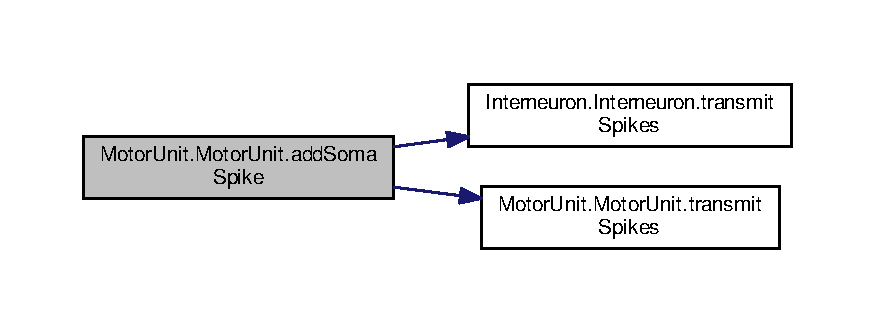
\includegraphics[width=350pt]{class_motor_unit_1_1_motor_unit_a6d597c703b3b469fbec7843a0f97c534_cgraph}
\end{center}
\end{figure}




Here is the caller graph for this function\+:\nopagebreak
\begin{figure}[H]
\begin{center}
\leavevmode
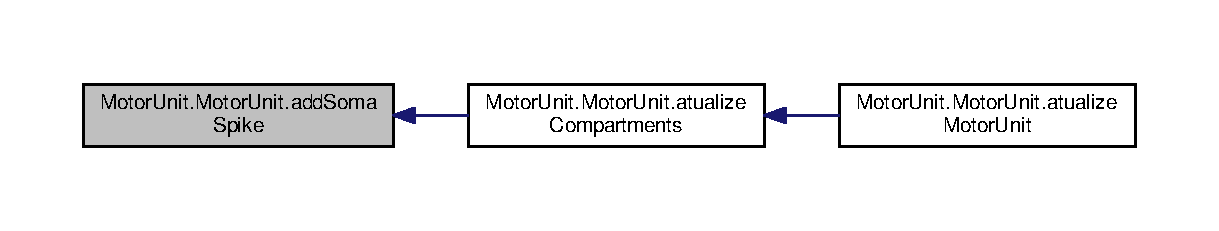
\includegraphics[width=350pt]{class_motor_unit_1_1_motor_unit_a6d597c703b3b469fbec7843a0f97c534_icgraph}
\end{center}
\end{figure}


\index{Motor\+Unit\+::\+Motor\+Unit@{Motor\+Unit\+::\+Motor\+Unit}!atualize\+Compartments@{atualize\+Compartments}}
\index{atualize\+Compartments@{atualize\+Compartments}!Motor\+Unit\+::\+Motor\+Unit@{Motor\+Unit\+::\+Motor\+Unit}}
\subsubsection[{\texorpdfstring{atualize\+Compartments(self, t)}{atualizeCompartments(self, t)}}]{\setlength{\rightskip}{0pt plus 5cm}def Motor\+Unit.\+Motor\+Unit.\+atualize\+Compartments (
\begin{DoxyParamCaption}
\item[{}]{self, }
\item[{}]{t}
\end{DoxyParamCaption}
)}\hypertarget{class_motor_unit_1_1_motor_unit_a666fa3bb4b8fb00f1217387a5ede5b7b}{}\label{class_motor_unit_1_1_motor_unit_a666fa3bb4b8fb00f1217387a5ede5b7b}


Atualize all neural compartments. 


\begin{DoxyItemize}
\item Inputs\+:
\begin{DoxyItemize}
\item {\bfseries t}\+: current instant, in ms. 
\end{DoxyItemize}
\end{DoxyItemize}

Definition at line 298 of file Motor\+Unit.\+py.



Here is the call graph for this function\+:
\nopagebreak
\begin{figure}[H]
\begin{center}
\leavevmode
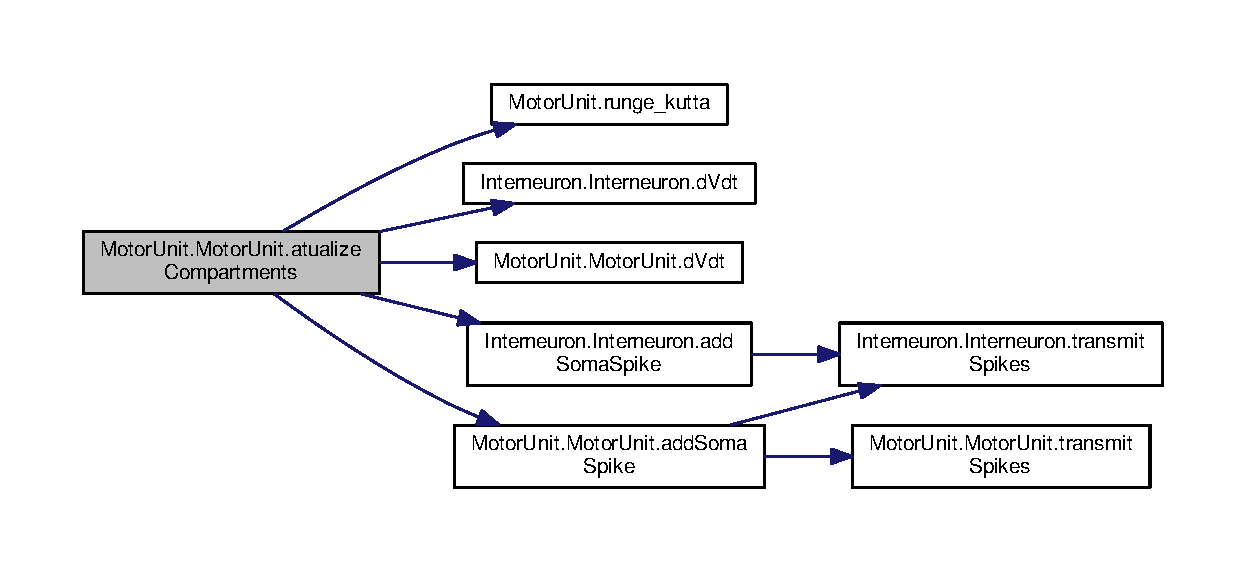
\includegraphics[width=350pt]{class_motor_unit_1_1_motor_unit_a666fa3bb4b8fb00f1217387a5ede5b7b_cgraph}
\end{center}
\end{figure}




Here is the caller graph for this function\+:\nopagebreak
\begin{figure}[H]
\begin{center}
\leavevmode
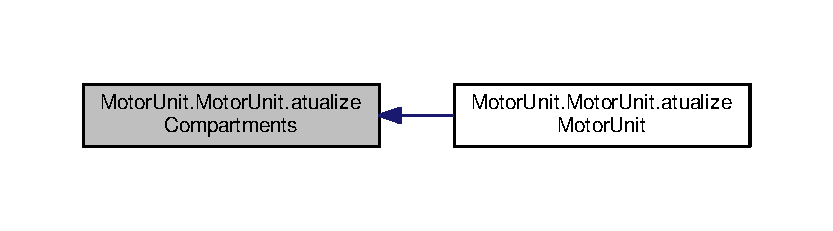
\includegraphics[width=350pt]{class_motor_unit_1_1_motor_unit_a666fa3bb4b8fb00f1217387a5ede5b7b_icgraph}
\end{center}
\end{figure}


\index{Motor\+Unit\+::\+Motor\+Unit@{Motor\+Unit\+::\+Motor\+Unit}!atualize\+Delay@{atualize\+Delay}}
\index{atualize\+Delay@{atualize\+Delay}!Motor\+Unit\+::\+Motor\+Unit@{Motor\+Unit\+::\+Motor\+Unit}}
\subsubsection[{\texorpdfstring{atualize\+Delay(self, t)}{atualizeDelay(self, t)}}]{\setlength{\rightskip}{0pt plus 5cm}def Motor\+Unit.\+Motor\+Unit.\+atualize\+Delay (
\begin{DoxyParamCaption}
\item[{}]{self, }
\item[{}]{t}
\end{DoxyParamCaption}
)}\hypertarget{class_motor_unit_1_1_motor_unit_a0aa5e024003845e3f48bc0e618068edc}{}\label{class_motor_unit_1_1_motor_unit_a0aa5e024003845e3f48bc0e618068edc}


Atualize the terminal spike train, by considering the Delay of the nerve. 


\begin{DoxyItemize}
\item Inputs\+:
\begin{DoxyItemize}
\item {\bfseries t}\+: current instant, in ms. 
\end{DoxyItemize}
\end{DoxyItemize}

Definition at line 352 of file Motor\+Unit.\+py.



Here is the caller graph for this function\+:\nopagebreak
\begin{figure}[H]
\begin{center}
\leavevmode
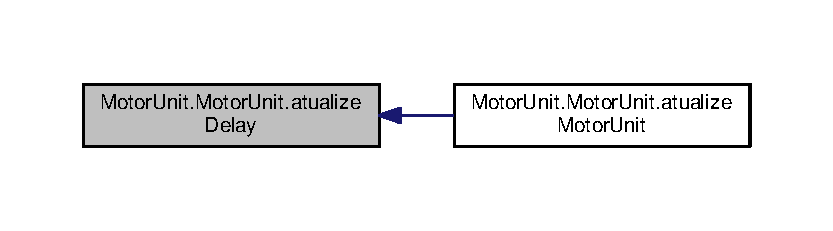
\includegraphics[width=350pt]{class_motor_unit_1_1_motor_unit_a0aa5e024003845e3f48bc0e618068edc_icgraph}
\end{center}
\end{figure}


\index{Motor\+Unit\+::\+Motor\+Unit@{Motor\+Unit\+::\+Motor\+Unit}!atualize\+Motor\+Unit@{atualize\+Motor\+Unit}}
\index{atualize\+Motor\+Unit@{atualize\+Motor\+Unit}!Motor\+Unit\+::\+Motor\+Unit@{Motor\+Unit\+::\+Motor\+Unit}}
\subsubsection[{\texorpdfstring{atualize\+Motor\+Unit(self, t)}{atualizeMotorUnit(self, t)}}]{\setlength{\rightskip}{0pt plus 5cm}def Motor\+Unit.\+Motor\+Unit.\+atualize\+Motor\+Unit (
\begin{DoxyParamCaption}
\item[{}]{self, }
\item[{}]{t}
\end{DoxyParamCaption}
)}\hypertarget{class_motor_unit_1_1_motor_unit_ab57693c2f49518b08639456595e92d87}{}\label{class_motor_unit_1_1_motor_unit_ab57693c2f49518b08639456595e92d87}


Atualize the dynamical and nondynamical (delay) parts of the motor unit. 


\begin{DoxyItemize}
\item Inputs\+:
\begin{DoxyItemize}
\item {\bfseries t}\+: current instant, in ms. 
\end{DoxyItemize}
\end{DoxyItemize}

Definition at line 286 of file Motor\+Unit.\+py.



Here is the call graph for this function\+:
\nopagebreak
\begin{figure}[H]
\begin{center}
\leavevmode
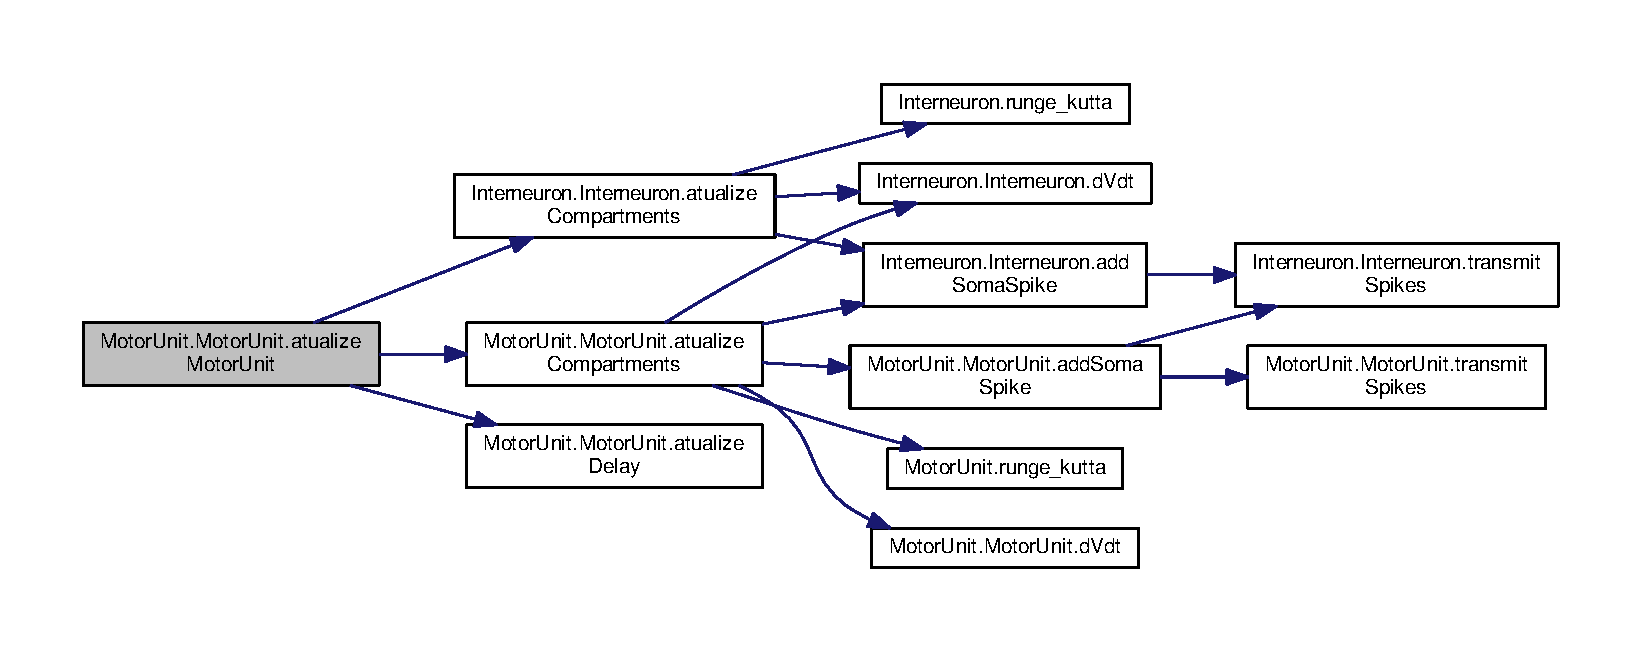
\includegraphics[width=350pt]{class_motor_unit_1_1_motor_unit_ab57693c2f49518b08639456595e92d87_cgraph}
\end{center}
\end{figure}


\index{Motor\+Unit\+::\+Motor\+Unit@{Motor\+Unit\+::\+Motor\+Unit}!d\+Vdt@{d\+Vdt}}
\index{d\+Vdt@{d\+Vdt}!Motor\+Unit\+::\+Motor\+Unit@{Motor\+Unit\+::\+Motor\+Unit}}
\subsubsection[{\texorpdfstring{d\+Vdt(self, t, V)}{dVdt(self, t, V)}}]{\setlength{\rightskip}{0pt plus 5cm}def Motor\+Unit.\+Motor\+Unit.\+d\+Vdt (
\begin{DoxyParamCaption}
\item[{}]{self, }
\item[{}]{t, }
\item[{}]{V}
\end{DoxyParamCaption}
)}\hypertarget{class_motor_unit_1_1_motor_unit_adf30fdef09ac21cfc2a261b762a7f618}{}\label{class_motor_unit_1_1_motor_unit_adf30fdef09ac21cfc2a261b762a7f618}


Compute the potential derivative of all compartments of the motor unit. 


\begin{DoxyItemize}
\item Inputs\+:
\begin{DoxyItemize}
\item {\bfseries t}\+: current instant, in ms.
\item {\bfseries V}\+: Vector with the current potential value of all neural compartments of the motor unit. 
\end{DoxyItemize}
\end{DoxyItemize}

Definition at line 321 of file Motor\+Unit.\+py.



Here is the caller graph for this function\+:\nopagebreak
\begin{figure}[H]
\begin{center}
\leavevmode
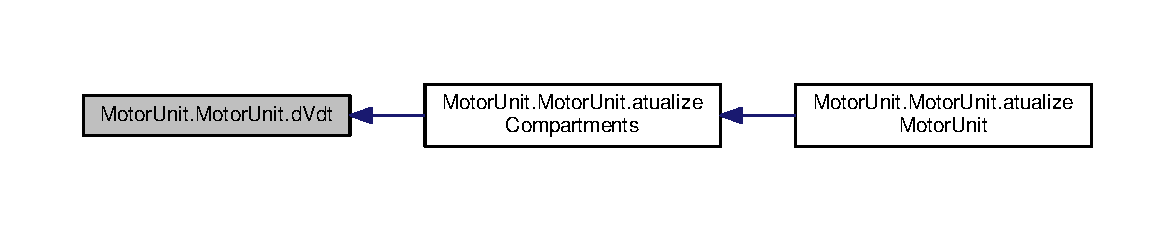
\includegraphics[width=350pt]{class_motor_unit_1_1_motor_unit_adf30fdef09ac21cfc2a261b762a7f618_icgraph}
\end{center}
\end{figure}


\index{Motor\+Unit\+::\+Motor\+Unit@{Motor\+Unit\+::\+Motor\+Unit}!transmit\+Spikes@{transmit\+Spikes}}
\index{transmit\+Spikes@{transmit\+Spikes}!Motor\+Unit\+::\+Motor\+Unit@{Motor\+Unit\+::\+Motor\+Unit}}
\subsubsection[{\texorpdfstring{transmit\+Spikes(self, t)}{transmitSpikes(self, t)}}]{\setlength{\rightskip}{0pt plus 5cm}def Motor\+Unit.\+Motor\+Unit.\+transmit\+Spikes (
\begin{DoxyParamCaption}
\item[{}]{self, }
\item[{}]{t}
\end{DoxyParamCaption}
)}\hypertarget{class_motor_unit_1_1_motor_unit_ac3d3e69bf0b75eef81a015005052f5d3}{}\label{class_motor_unit_1_1_motor_unit_ac3d3e69bf0b75eef81a015005052f5d3}

\begin{DoxyItemize}
\item Inputs\+:
\begin{DoxyItemize}
\item {\bfseries t}\+: current instant, in ms. 
\end{DoxyItemize}
\end{DoxyItemize}

Definition at line 362 of file Motor\+Unit.\+py.



Here is the caller graph for this function\+:
\nopagebreak
\begin{figure}[H]
\begin{center}
\leavevmode
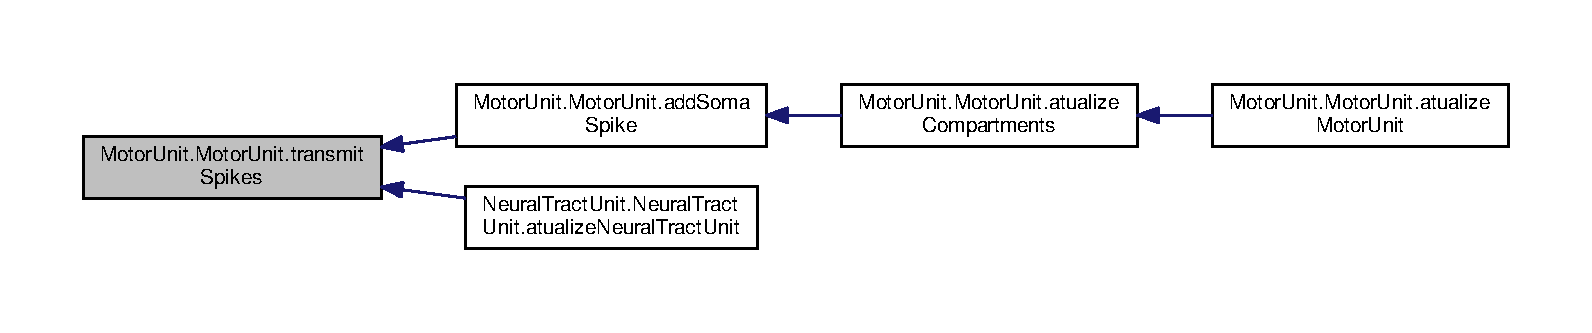
\includegraphics[width=350pt]{class_motor_unit_1_1_motor_unit_ac3d3e69bf0b75eef81a015005052f5d3_icgraph}
\end{center}
\end{figure}




\subsection{Member Data Documentation}
\index{Motor\+Unit\+::\+Motor\+Unit@{Motor\+Unit\+::\+Motor\+Unit}!b\+Sat@{b\+Sat}}
\index{b\+Sat@{b\+Sat}!Motor\+Unit\+::\+Motor\+Unit@{Motor\+Unit\+::\+Motor\+Unit}}
\subsubsection[{\texorpdfstring{b\+Sat}{bSat}}]{\setlength{\rightskip}{0pt plus 5cm}Motor\+Unit.\+Motor\+Unit.\+b\+Sat}\hypertarget{class_motor_unit_1_1_motor_unit_a2256c241b36e0181e3530e6f791545a0}{}\label{class_motor_unit_1_1_motor_unit_a2256c241b36e0181e3530e6f791545a0}


Parameter of the saturation. 



Definition at line 267 of file Motor\+Unit.\+py.

\index{Motor\+Unit\+::\+Motor\+Unit@{Motor\+Unit\+::\+Motor\+Unit}!capacitance\+Inv@{capacitance\+Inv}}
\index{capacitance\+Inv@{capacitance\+Inv}!Motor\+Unit\+::\+Motor\+Unit@{Motor\+Unit\+::\+Motor\+Unit}}
\subsubsection[{\texorpdfstring{capacitance\+Inv}{capacitanceInv}}]{\setlength{\rightskip}{0pt plus 5cm}Motor\+Unit.\+Motor\+Unit.\+capacitance\+Inv}\hypertarget{class_motor_unit_1_1_motor_unit_a0cf2afb5bd12374db56b9d9a5a1671e6}{}\label{class_motor_unit_1_1_motor_unit_a0cf2afb5bd12374db56b9d9a5a1671e6}


Vector with the inverse of the capacitance of all compartments. 



Definition at line 219 of file Motor\+Unit.\+py.

\index{Motor\+Unit\+::\+Motor\+Unit@{Motor\+Unit\+::\+Motor\+Unit}!compartment@{compartment}}
\index{compartment@{compartment}!Motor\+Unit\+::\+Motor\+Unit@{Motor\+Unit\+::\+Motor\+Unit}}
\subsubsection[{\texorpdfstring{compartment}{compartment}}]{\setlength{\rightskip}{0pt plus 5cm}Motor\+Unit.\+Motor\+Unit.\+compartment}\hypertarget{class_motor_unit_1_1_motor_unit_a6d4da7327031b3cb9c7041a4a790e524}{}\label{class_motor_unit_1_1_motor_unit_a6d4da7327031b3cb9c7041a4a790e524}


Vector of \hyperlink{namespace_compartment}{Compartment} of the Motor Unit. 



Definition at line 187 of file Motor\+Unit.\+py.

\index{Motor\+Unit\+::\+Motor\+Unit@{Motor\+Unit\+::\+Motor\+Unit}!comp\+Number@{comp\+Number}}
\index{comp\+Number@{comp\+Number}!Motor\+Unit\+::\+Motor\+Unit@{Motor\+Unit\+::\+Motor\+Unit}}
\subsubsection[{\texorpdfstring{comp\+Number}{compNumber}}]{\setlength{\rightskip}{0pt plus 5cm}Motor\+Unit.\+Motor\+Unit.\+comp\+Number}\hypertarget{class_motor_unit_1_1_motor_unit_afe7281fb12c41102980b6b48d5a49713}{}\label{class_motor_unit_1_1_motor_unit_afe7281fb12c41102980b6b48d5a49713}


Number of compartments. 



Definition at line 197 of file Motor\+Unit.\+py.

\index{Motor\+Unit\+::\+Motor\+Unit@{Motor\+Unit\+::\+Motor\+Unit}!conf@{conf}}
\index{conf@{conf}!Motor\+Unit\+::\+Motor\+Unit@{Motor\+Unit\+::\+Motor\+Unit}}
\subsubsection[{\texorpdfstring{conf}{conf}}]{\setlength{\rightskip}{0pt plus 5cm}Motor\+Unit.\+Motor\+Unit.\+conf}\hypertarget{class_motor_unit_1_1_motor_unit_a10539f5129881188923f3a3a164d2cba}{}\label{class_motor_unit_1_1_motor_unit_a10539f5129881188923f3a3a164d2cba}


\hyperlink{namespace_configuration}{Configuration} object with the simulation parameters. 



Definition at line 170 of file Motor\+Unit.\+py.

\index{Motor\+Unit\+::\+Motor\+Unit@{Motor\+Unit\+::\+Motor\+Unit}!Delay@{Delay}}
\index{Delay@{Delay}!Motor\+Unit\+::\+Motor\+Unit@{Motor\+Unit\+::\+Motor\+Unit}}
\subsubsection[{\texorpdfstring{Delay}{Delay}}]{\setlength{\rightskip}{0pt plus 5cm}Motor\+Unit.\+Motor\+Unit.\+Delay}\hypertarget{class_motor_unit_1_1_motor_unit_abe82ffa1e293d10225b67870a962eab8}{}\label{class_motor_unit_1_1_motor_unit_abe82ffa1e293d10225b67870a962eab8}


\hyperlink{namespace_axon_delay}{Axon\+Delay} object of the motor unit. 



Definition at line 252 of file Motor\+Unit.\+py.

\index{Motor\+Unit\+::\+Motor\+Unit@{Motor\+Unit\+::\+Motor\+Unit}!G@{G}}
\index{G@{G}!Motor\+Unit\+::\+Motor\+Unit@{Motor\+Unit\+::\+Motor\+Unit}}
\subsubsection[{\texorpdfstring{G}{G}}]{\setlength{\rightskip}{0pt plus 5cm}Motor\+Unit.\+Motor\+Unit.\+G}\hypertarget{class_motor_unit_1_1_motor_unit_a9b9f157ab92b47470ca7ec6bd3473dd3}{}\label{class_motor_unit_1_1_motor_unit_a9b9f157ab92b47470ca7ec6bd3473dd3}


Matrix of the conductance of the motoneuron. 

Multiplied by the vector self.\+v\+\_\+mV, results in the passive currents of each compartment. 

Definition at line 234 of file Motor\+Unit.\+py.

\index{Motor\+Unit\+::\+Motor\+Unit@{Motor\+Unit\+::\+Motor\+Unit}!i\+Injected@{i\+Injected}}
\index{i\+Injected@{i\+Injected}!Motor\+Unit\+::\+Motor\+Unit@{Motor\+Unit\+::\+Motor\+Unit}}
\subsubsection[{\texorpdfstring{i\+Injected}{iInjected}}]{\setlength{\rightskip}{0pt plus 5cm}Motor\+Unit.\+Motor\+Unit.\+i\+Injected}\hypertarget{class_motor_unit_1_1_motor_unit_a06045eca379d38892670a491dbac0829}{}\label{class_motor_unit_1_1_motor_unit_a06045eca379d38892670a491dbac0829}


Vector with the current, in nA, injected in each compartment. 



Definition at line 225 of file Motor\+Unit.\+py.

\index{Motor\+Unit\+::\+Motor\+Unit@{Motor\+Unit\+::\+Motor\+Unit}!i\+Ionic@{i\+Ionic}}
\index{i\+Ionic@{i\+Ionic}!Motor\+Unit\+::\+Motor\+Unit@{Motor\+Unit\+::\+Motor\+Unit}}
\subsubsection[{\texorpdfstring{i\+Ionic}{iIonic}}]{\setlength{\rightskip}{0pt plus 5cm}Motor\+Unit.\+Motor\+Unit.\+i\+Ionic}\hypertarget{class_motor_unit_1_1_motor_unit_a0541858216e7d01582312f9a7a99d595}{}\label{class_motor_unit_1_1_motor_unit_a0541858216e7d01582312f9a7a99d595}


Vector with current, in nA, of each compartment coming from other elements of the model. 

For example from ionic channels and synapses. 

Definition at line 223 of file Motor\+Unit.\+py.

\index{Motor\+Unit\+::\+Motor\+Unit@{Motor\+Unit\+::\+Motor\+Unit}!index@{index}}
\index{index@{index}!Motor\+Unit\+::\+Motor\+Unit@{Motor\+Unit\+::\+Motor\+Unit}}
\subsubsection[{\texorpdfstring{index}{index}}]{\setlength{\rightskip}{0pt plus 5cm}Motor\+Unit.\+Motor\+Unit.\+index}\hypertarget{class_motor_unit_1_1_motor_unit_a4f3205a9273aabb92d425992d91a1848}{}\label{class_motor_unit_1_1_motor_unit_a4f3205a9273aabb92d425992d91a1848}


Integer corresponding to the motor unit order in the pool, according to the Henneman\textquotesingle{}s principle (size principle). 



Definition at line 185 of file Motor\+Unit.\+py.

\index{Motor\+Unit\+::\+Motor\+Unit@{Motor\+Unit\+::\+Motor\+Unit}!indices\+Of\+Synapses\+On\+Target@{indices\+Of\+Synapses\+On\+Target}}
\index{indices\+Of\+Synapses\+On\+Target@{indices\+Of\+Synapses\+On\+Target}!Motor\+Unit\+::\+Motor\+Unit@{Motor\+Unit\+::\+Motor\+Unit}}
\subsubsection[{\texorpdfstring{indices\+Of\+Synapses\+On\+Target}{indicesOfSynapsesOnTarget}}]{\setlength{\rightskip}{0pt plus 5cm}Motor\+Unit.\+Motor\+Unit.\+indices\+Of\+Synapses\+On\+Target}\hypertarget{class_motor_unit_1_1_motor_unit_a9b53efb19f9b1a050ef1c21af4316755}{}\label{class_motor_unit_1_1_motor_unit_a9b53efb19f9b1a050ef1c21af4316755}


Definition at line 277 of file Motor\+Unit.\+py.

\index{Motor\+Unit\+::\+Motor\+Unit@{Motor\+Unit\+::\+Motor\+Unit}!kind@{kind}}
\index{kind@{kind}!Motor\+Unit\+::\+Motor\+Unit@{Motor\+Unit\+::\+Motor\+Unit}}
\subsubsection[{\texorpdfstring{kind}{kind}}]{\setlength{\rightskip}{0pt plus 5cm}Motor\+Unit.\+Motor\+Unit.\+kind}\hypertarget{class_motor_unit_1_1_motor_unit_a08ed5171ba46e0b1ea5bc7d08296c612}{}\label{class_motor_unit_1_1_motor_unit_a08ed5171ba46e0b1ea5bc7d08296c612}


String with the type of the motor unit. 

It can be {\itshape S} (slow), {\itshape FR} (fast and resistant) and $\ast$\+F\+F$\ast$$\ast$ (fast and fatigable). 

Definition at line 175 of file Motor\+Unit.\+py.

\index{Motor\+Unit\+::\+Motor\+Unit@{Motor\+Unit\+::\+Motor\+Unit}!M\+N\+Ref\+Per\+\_\+ms@{M\+N\+Ref\+Per\+\_\+ms}}
\index{M\+N\+Ref\+Per\+\_\+ms@{M\+N\+Ref\+Per\+\_\+ms}!Motor\+Unit\+::\+Motor\+Unit@{Motor\+Unit\+::\+Motor\+Unit}}
\subsubsection[{\texorpdfstring{M\+N\+Ref\+Per\+\_\+ms}{MNRefPer_ms}}]{\setlength{\rightskip}{0pt plus 5cm}Motor\+Unit.\+Motor\+Unit.\+M\+N\+Ref\+Per\+\_\+ms}\hypertarget{class_motor_unit_1_1_motor_unit_abbdaa195ac00926d96d509ae01dcda05}{}\label{class_motor_unit_1_1_motor_unit_abbdaa195ac00926d96d509ae01dcda05}


Refractory period, in ms, of the motoneuron. 



Definition at line 241 of file Motor\+Unit.\+py.

\index{Motor\+Unit\+::\+Motor\+Unit@{Motor\+Unit\+::\+Motor\+Unit}!nerve@{nerve}}
\index{nerve@{nerve}!Motor\+Unit\+::\+Motor\+Unit@{Motor\+Unit\+::\+Motor\+Unit}}
\subsubsection[{\texorpdfstring{nerve}{nerve}}]{\setlength{\rightskip}{0pt plus 5cm}Motor\+Unit.\+Motor\+Unit.\+nerve}\hypertarget{class_motor_unit_1_1_motor_unit_a754ee6b88fc2a09899da9f9b13bfbf59}{}\label{class_motor_unit_1_1_motor_unit_a754ee6b88fc2a09899da9f9b13bfbf59}


String with type of the nerve. 

It can be P\+TN (posterior tibial nerve) or C\+PN (common peroneal nerve). 

Definition at line 247 of file Motor\+Unit.\+py.

\index{Motor\+Unit\+::\+Motor\+Unit@{Motor\+Unit\+::\+Motor\+Unit}!position\+\_\+mm@{position\+\_\+mm}}
\index{position\+\_\+mm@{position\+\_\+mm}!Motor\+Unit\+::\+Motor\+Unit@{Motor\+Unit\+::\+Motor\+Unit}}
\subsubsection[{\texorpdfstring{position\+\_\+mm}{position_mm}}]{\setlength{\rightskip}{0pt plus 5cm}Motor\+Unit.\+Motor\+Unit.\+position\+\_\+mm}\hypertarget{class_motor_unit_1_1_motor_unit_a9b1938bcbaa8c89ef47e0b915ab4cd39}{}\label{class_motor_unit_1_1_motor_unit_a9b1938bcbaa8c89ef47e0b915ab4cd39}


Anatomical position of the neuron, in mm. 



Definition at line 192 of file Motor\+Unit.\+py.

\index{Motor\+Unit\+::\+Motor\+Unit@{Motor\+Unit\+::\+Motor\+Unit}!soma\+Index@{soma\+Index}}
\index{soma\+Index@{soma\+Index}!Motor\+Unit\+::\+Motor\+Unit@{Motor\+Unit\+::\+Motor\+Unit}}
\subsubsection[{\texorpdfstring{soma\+Index}{somaIndex}}]{\setlength{\rightskip}{0pt plus 5cm}Motor\+Unit.\+Motor\+Unit.\+soma\+Index}\hypertarget{class_motor_unit_1_1_motor_unit_a7cd2be92814b5892bdd18dafd824da9f}{}\label{class_motor_unit_1_1_motor_unit_a7cd2be92814b5892bdd18dafd824da9f}


index of the soma compartment. 



Definition at line 238 of file Motor\+Unit.\+py.

\index{Motor\+Unit\+::\+Motor\+Unit@{Motor\+Unit\+::\+Motor\+Unit}!soma\+Spike\+Train@{soma\+Spike\+Train}}
\index{soma\+Spike\+Train@{soma\+Spike\+Train}!Motor\+Unit\+::\+Motor\+Unit@{Motor\+Unit\+::\+Motor\+Unit}}
\subsubsection[{\texorpdfstring{soma\+Spike\+Train}{somaSpikeTrain}}]{\setlength{\rightskip}{0pt plus 5cm}Motor\+Unit.\+Motor\+Unit.\+soma\+Spike\+Train}\hypertarget{class_motor_unit_1_1_motor_unit_a8c86d98daa6c509e226ab165fa92515f}{}\label{class_motor_unit_1_1_motor_unit_a8c86d98daa6c509e226ab165fa92515f}


Vector with the instants of spikes at the soma. 



Definition at line 183 of file Motor\+Unit.\+py.

\index{Motor\+Unit\+::\+Motor\+Unit@{Motor\+Unit\+::\+Motor\+Unit}!Synapses\+Out@{Synapses\+Out}}
\index{Synapses\+Out@{Synapses\+Out}!Motor\+Unit\+::\+Motor\+Unit@{Motor\+Unit\+::\+Motor\+Unit}}
\subsubsection[{\texorpdfstring{Synapses\+Out}{SynapsesOut}}]{\setlength{\rightskip}{0pt plus 5cm}Motor\+Unit.\+Motor\+Unit.\+Synapses\+Out}\hypertarget{class_motor_unit_1_1_motor_unit_a898cd628506c666bf326b02436be0750}{}\label{class_motor_unit_1_1_motor_unit_a898cd628506c666bf326b02436be0750}


E\+MG data. 

Build synapses 

Definition at line 275 of file Motor\+Unit.\+py.

\index{Motor\+Unit\+::\+Motor\+Unit@{Motor\+Unit\+::\+Motor\+Unit}!terminal\+Spike\+Train@{terminal\+Spike\+Train}}
\index{terminal\+Spike\+Train@{terminal\+Spike\+Train}!Motor\+Unit\+::\+Motor\+Unit@{Motor\+Unit\+::\+Motor\+Unit}}
\subsubsection[{\texorpdfstring{terminal\+Spike\+Train}{terminalSpikeTrain}}]{\setlength{\rightskip}{0pt plus 5cm}Motor\+Unit.\+Motor\+Unit.\+terminal\+Spike\+Train}\hypertarget{class_motor_unit_1_1_motor_unit_a2e33990aaab69454943aa00db6b8d2eb}{}\label{class_motor_unit_1_1_motor_unit_a2e33990aaab69454943aa00db6b8d2eb}


Vector with the instants of spikes at the terminal. 



Definition at line 256 of file Motor\+Unit.\+py.

\index{Motor\+Unit\+::\+Motor\+Unit@{Motor\+Unit\+::\+Motor\+Unit}!threshold\+\_\+mV@{threshold\+\_\+mV}}
\index{threshold\+\_\+mV@{threshold\+\_\+mV}!Motor\+Unit\+::\+Motor\+Unit@{Motor\+Unit\+::\+Motor\+Unit}}
\subsubsection[{\texorpdfstring{threshold\+\_\+mV}{threshold_mV}}]{\setlength{\rightskip}{0pt plus 5cm}Motor\+Unit.\+Motor\+Unit.\+threshold\+\_\+mV}\hypertarget{class_motor_unit_1_1_motor_unit_affbd0b90f1dce6a0f929775e54f8c212}{}\label{class_motor_unit_1_1_motor_unit_affbd0b90f1dce6a0f929775e54f8c212}


Value of the membrane potential, in mV, that is considered a spike. 



Definition at line 189 of file Motor\+Unit.\+py.

\index{Motor\+Unit\+::\+Motor\+Unit@{Motor\+Unit\+::\+Motor\+Unit}!transmit\+Spikes\+Through\+Synapses@{transmit\+Spikes\+Through\+Synapses}}
\index{transmit\+Spikes\+Through\+Synapses@{transmit\+Spikes\+Through\+Synapses}!Motor\+Unit\+::\+Motor\+Unit@{Motor\+Unit\+::\+Motor\+Unit}}
\subsubsection[{\texorpdfstring{transmit\+Spikes\+Through\+Synapses}{transmitSpikesThroughSynapses}}]{\setlength{\rightskip}{0pt plus 5cm}Motor\+Unit.\+Motor\+Unit.\+transmit\+Spikes\+Through\+Synapses}\hypertarget{class_motor_unit_1_1_motor_unit_a30fc94e8b9f24b75770bb903e20f1961}{}\label{class_motor_unit_1_1_motor_unit_a30fc94e8b9f24b75770bb903e20f1961}


Definition at line 276 of file Motor\+Unit.\+py.

\index{Motor\+Unit\+::\+Motor\+Unit@{Motor\+Unit\+::\+Motor\+Unit}!t\+Soma\+Spike@{t\+Soma\+Spike}}
\index{t\+Soma\+Spike@{t\+Soma\+Spike}!Motor\+Unit\+::\+Motor\+Unit@{Motor\+Unit\+::\+Motor\+Unit}}
\subsubsection[{\texorpdfstring{t\+Soma\+Spike}{tSomaSpike}}]{\setlength{\rightskip}{0pt plus 5cm}Motor\+Unit.\+Motor\+Unit.\+t\+Soma\+Spike}\hypertarget{class_motor_unit_1_1_motor_unit_abca82ec2c7312bb475989bb45e82ca28}{}\label{class_motor_unit_1_1_motor_unit_abca82ec2c7312bb475989bb45e82ca28}


The instant of the last spike of the Motor unit at the Soma compartment. 



Definition at line 180 of file Motor\+Unit.\+py.

\index{Motor\+Unit\+::\+Motor\+Unit@{Motor\+Unit\+::\+Motor\+Unit}!Twitch\+Amp\+\_\+N@{Twitch\+Amp\+\_\+N}}
\index{Twitch\+Amp\+\_\+N@{Twitch\+Amp\+\_\+N}!Motor\+Unit\+::\+Motor\+Unit@{Motor\+Unit\+::\+Motor\+Unit}}
\subsubsection[{\texorpdfstring{Twitch\+Amp\+\_\+N}{TwitchAmp_N}}]{\setlength{\rightskip}{0pt plus 5cm}Motor\+Unit.\+Motor\+Unit.\+Twitch\+Amp\+\_\+N}\hypertarget{class_motor_unit_1_1_motor_unit_ad14af870eb3dd7468041853f2c6e8cab}{}\label{class_motor_unit_1_1_motor_unit_ad14af870eb3dd7468041853f2c6e8cab}


Amplitude of the muscle unit twitch, in N. 



Definition at line 265 of file Motor\+Unit.\+py.

\index{Motor\+Unit\+::\+Motor\+Unit@{Motor\+Unit\+::\+Motor\+Unit}!Twitch\+Tc\+\_\+ms@{Twitch\+Tc\+\_\+ms}}
\index{Twitch\+Tc\+\_\+ms@{Twitch\+Tc\+\_\+ms}!Motor\+Unit\+::\+Motor\+Unit@{Motor\+Unit\+::\+Motor\+Unit}}
\subsubsection[{\texorpdfstring{Twitch\+Tc\+\_\+ms}{TwitchTc_ms}}]{\setlength{\rightskip}{0pt plus 5cm}Motor\+Unit.\+Motor\+Unit.\+Twitch\+Tc\+\_\+ms}\hypertarget{class_motor_unit_1_1_motor_unit_a083581c89ebb964e58721667307dd2bc}{}\label{class_motor_unit_1_1_motor_unit_a083581c89ebb964e58721667307dd2bc}


Contraction time of the twitch muscle unit, in ms. 



Definition at line 263 of file Motor\+Unit.\+py.

\index{Motor\+Unit\+::\+Motor\+Unit@{Motor\+Unit\+::\+Motor\+Unit}!tw\+Tet@{tw\+Tet}}
\index{tw\+Tet@{tw\+Tet}!Motor\+Unit\+::\+Motor\+Unit@{Motor\+Unit\+::\+Motor\+Unit}}
\subsubsection[{\texorpdfstring{tw\+Tet}{twTet}}]{\setlength{\rightskip}{0pt plus 5cm}Motor\+Unit.\+Motor\+Unit.\+tw\+Tet}\hypertarget{class_motor_unit_1_1_motor_unit_a2a466c5f2f798901c1c438f9d57c2221}{}\label{class_motor_unit_1_1_motor_unit_a2a466c5f2f798901c1c438f9d57c2221}


Twitch-\/ tetanus relationship. 



Definition at line 269 of file Motor\+Unit.\+py.

\index{Motor\+Unit\+::\+Motor\+Unit@{Motor\+Unit\+::\+Motor\+Unit}!v\+\_\+mV@{v\+\_\+mV}}
\index{v\+\_\+mV@{v\+\_\+mV}!Motor\+Unit\+::\+Motor\+Unit@{Motor\+Unit\+::\+Motor\+Unit}}
\subsubsection[{\texorpdfstring{v\+\_\+mV}{v_mV}}]{\setlength{\rightskip}{0pt plus 5cm}Motor\+Unit.\+Motor\+Unit.\+v\+\_\+mV}\hypertarget{class_motor_unit_1_1_motor_unit_aa8968f89250895ae2ae572e9106709f2}{}\label{class_motor_unit_1_1_motor_unit_aa8968f89250895ae2ae572e9106709f2}


Vector with membrane potential,in mV, of all compartments. 



Definition at line 199 of file Motor\+Unit.\+py.



The documentation for this class was generated from the following file\+:\begin{DoxyCompactItemize}
\item 
\hyperlink{_motor_unit_8py}{Motor\+Unit.\+py}\end{DoxyCompactItemize}

\hypertarget{class_motor_unit_pool_1_1_motor_unit_pool}{\section{Motor\-Unit\-Pool.\-Motor\-Unit\-Pool Class Reference}
\label{class_motor_unit_pool_1_1_motor_unit_pool}\index{Motor\-Unit\-Pool.\-Motor\-Unit\-Pool@{Motor\-Unit\-Pool.\-Motor\-Unit\-Pool}}
}


Class that implements a motor unit pool.  


\subsection*{Public Member Functions}
\begin{DoxyCompactItemize}
\item 
def \hyperlink{class_motor_unit_pool_1_1_motor_unit_pool_a627cffa9977225e58194d63a338059dc}{\-\_\-\-\_\-init\-\_\-\-\_\-}
\begin{DoxyCompactList}\small\item\em Constructor. \end{DoxyCompactList}\item 
def \hyperlink{class_motor_unit_pool_1_1_motor_unit_pool_ae525c6bba27837f09d2a767544780b0f}{atualize\-Motor\-Unit\-Pool}
\item 
def \hyperlink{class_motor_unit_pool_1_1_motor_unit_pool_a03b7c1202f680bd8ba3af9b0b06bd71c}{atualize\-Activation\-Signal}
\item 
def \hyperlink{class_motor_unit_pool_1_1_motor_unit_pool_a8fbb182559fe08eb45800271655b711f}{atualize\-Force\-No\-Hill}
\begin{DoxyCompactList}\small\item\em Compute the muscle force when no muscle dynamics (Hill model) is used. \end{DoxyCompactList}\item 
def \hyperlink{class_motor_unit_pool_1_1_motor_unit_pool_a156ffc40be4c7c37f79905fa58b017e5}{list\-Spikes}
\end{DoxyCompactItemize}
\subsection*{Public Attributes}
\begin{DoxyCompactItemize}
\item 
\hyperlink{class_motor_unit_pool_1_1_motor_unit_pool_aeb57d0463ad56a16b166d00dc6079b95}{kind}
\begin{DoxyCompactList}\small\item\em Indicates that is Motor Unit pool. \end{DoxyCompactList}\item 
\hyperlink{class_motor_unit_pool_1_1_motor_unit_pool_a3b2ee8f3e5500bfdc8fa731a5cb7d622}{conf}
\begin{DoxyCompactList}\small\item\em \hyperlink{namespace_configuration}{Configuration} object with the simulation parameters. \end{DoxyCompactList}\item 
\hyperlink{class_motor_unit_pool_1_1_motor_unit_pool_a832364dc014aa8a1b2947abfe063f626}{pool}
\begin{DoxyCompactList}\small\item\em String with Motor unit pool to which the motor unit belongs. \end{DoxyCompactList}\item 
\hyperlink{class_motor_unit_pool_1_1_motor_unit_pool_aa5884530baaa20f46007805bc574407d}{M\-Unumber}
\begin{DoxyCompactList}\small\item\em Number of motor units. \end{DoxyCompactList}\item 
\hyperlink{class_motor_unit_pool_1_1_motor_unit_pool_a1b14c831606c27efae62f1468850393b}{unit}
\begin{DoxyCompactList}\small\item\em List of \hyperlink{namespace_motor_unit}{Motor\-Unit} objects. \end{DoxyCompactList}\item 
\hyperlink{class_motor_unit_pool_1_1_motor_unit_pool_a3790757a111061662ad0f98120b25e69}{pool\-Soma\-Spikes}
\begin{DoxyCompactList}\small\item\em Vector with the instants of spikes in the soma compartment, in ms. \end{DoxyCompactList}\item 
\hyperlink{class_motor_unit_pool_1_1_motor_unit_pool_a4f0b93df27eb6303fa1a3d49653d4fd3}{pool\-Terminal\-Spikes}
\begin{DoxyCompactList}\small\item\em Vector with the instants of spikes in the terminal, in ms. \end{DoxyCompactList}\item 
\hyperlink{class_motor_unit_pool_1_1_motor_unit_pool_abaa7680d0691fac81f66b200dfcfd203}{activation\-Model}
\begin{DoxyCompactList}\small\item\em Model of the activation signal. \end{DoxyCompactList}\item 
\hyperlink{class_motor_unit_pool_1_1_motor_unit_pool_ad03b9e215e833188060e90bc4392d42b}{Act\-Matrix}
\item 
\hyperlink{class_motor_unit_pool_1_1_motor_unit_pool_ac72c67b4a1f6134965ab77e2d798b5a4}{an}
\item 
\hyperlink{class_motor_unit_pool_1_1_motor_unit_pool_a467ac7b080b79b9515d5846d75e95d1c}{activation\-\_\-non\-Sat}
\item 
\hyperlink{class_motor_unit_pool_1_1_motor_unit_pool_a4e107835e34b4f56d06b9b28c143fe40}{b\-Sat}
\item 
\hyperlink{class_motor_unit_pool_1_1_motor_unit_pool_a785a769c5b4824603a24339e4f0d8dfe}{tw\-Tet}
\item 
\hyperlink{class_motor_unit_pool_1_1_motor_unit_pool_a03538b06e7220f9d48c7306ed6508c05}{twitch\-Amp\-\_\-\-N}
\item 
\hyperlink{class_motor_unit_pool_1_1_motor_unit_pool_ac475d1369c38d0bc5064c7243b4e1d44}{activation\-\_\-\-Sat}
\item 
\hyperlink{class_motor_unit_pool_1_1_motor_unit_pool_a48b53d4f838ca8cfe2bc41c8308f2060}{dirac\-Delta\-Value}
\item 
\hyperlink{class_motor_unit_pool_1_1_motor_unit_pool_a97011c17140c45a42a00105279f014ad}{force}
\item 
\hyperlink{class_motor_unit_pool_1_1_motor_unit_pool_a963061fdcfee8f9dc33e4d6f130ea59b}{hill\-Model}
\item 
\hyperlink{class_motor_unit_pool_1_1_motor_unit_pool_a21f9a6a5d113b5b0f67a3557c47ebd5a}{atualize\-Force}
\item 
\hyperlink{class_motor_unit_pool_1_1_motor_unit_pool_ab5659e1c9355ecf529d9b8be8cbf6d65}{time\-Index}
\end{DoxyCompactItemize}


\subsection{Detailed Description}
Class that implements a motor unit pool. 

Encompasses a set of motor units that controls a single muscle. 

Definition at line 40 of file Motor\-Unit\-Pool.\-py.



\subsection{Constructor \& Destructor Documentation}
\hypertarget{class_motor_unit_pool_1_1_motor_unit_pool_a627cffa9977225e58194d63a338059dc}{\index{Motor\-Unit\-Pool\-::\-Motor\-Unit\-Pool@{Motor\-Unit\-Pool\-::\-Motor\-Unit\-Pool}!\-\_\-\-\_\-init\-\_\-\-\_\-@{\-\_\-\-\_\-init\-\_\-\-\_\-}}
\index{\-\_\-\-\_\-init\-\_\-\-\_\-@{\-\_\-\-\_\-init\-\_\-\-\_\-}!MotorUnitPool::MotorUnitPool@{Motor\-Unit\-Pool\-::\-Motor\-Unit\-Pool}}
\subsubsection[{\-\_\-\-\_\-init\-\_\-\-\_\-}]{\setlength{\rightskip}{0pt plus 5cm}def Motor\-Unit\-Pool.\-Motor\-Unit\-Pool.\-\_\-\-\_\-init\-\_\-\-\_\- (
\begin{DoxyParamCaption}
\item[{}]{self, }
\item[{}]{conf, }
\item[{}]{pool}
\end{DoxyParamCaption}
)}}\label{class_motor_unit_pool_1_1_motor_unit_pool_a627cffa9977225e58194d63a338059dc}


Constructor. 


\begin{DoxyItemize}
\item Inputs\-:
\begin{DoxyItemize}
\item {\bfseries conf}\-: \hyperlink{namespace_configuration}{Configuration} object with the simulation parameters.
\item {\bfseries pool}\-: string with Motor unit pool to which the motor unit belongs. 
\end{DoxyItemize}
\end{DoxyItemize}

Definition at line 52 of file Motor\-Unit\-Pool.\-py.



\subsection{Member Function Documentation}
\hypertarget{class_motor_unit_pool_1_1_motor_unit_pool_a03b7c1202f680bd8ba3af9b0b06bd71c}{\index{Motor\-Unit\-Pool\-::\-Motor\-Unit\-Pool@{Motor\-Unit\-Pool\-::\-Motor\-Unit\-Pool}!atualize\-Activation\-Signal@{atualize\-Activation\-Signal}}
\index{atualize\-Activation\-Signal@{atualize\-Activation\-Signal}!MotorUnitPool::MotorUnitPool@{Motor\-Unit\-Pool\-::\-Motor\-Unit\-Pool}}
\subsubsection[{atualize\-Activation\-Signal}]{\setlength{\rightskip}{0pt plus 5cm}def Motor\-Unit\-Pool.\-Motor\-Unit\-Pool.\-atualize\-Activation\-Signal (
\begin{DoxyParamCaption}
\item[{}]{self, }
\item[{}]{t}
\end{DoxyParamCaption}
)}}\label{class_motor_unit_pool_1_1_motor_unit_pool_a03b7c1202f680bd8ba3af9b0b06bd71c}


Definition at line 136 of file Motor\-Unit\-Pool.\-py.



Here is the call graph for this function\-:\nopagebreak
\begin{figure}[H]
\begin{center}
\leavevmode
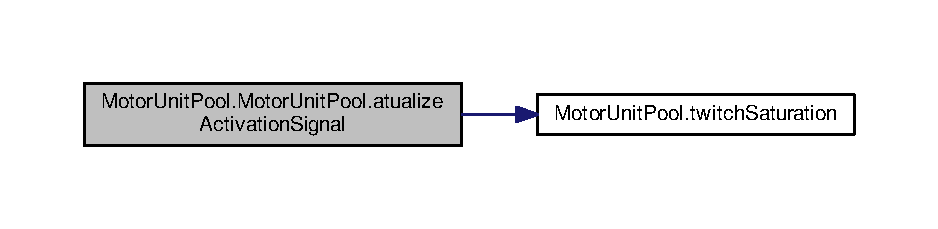
\includegraphics[width=350pt]{class_motor_unit_pool_1_1_motor_unit_pool_a03b7c1202f680bd8ba3af9b0b06bd71c_cgraph}
\end{center}
\end{figure}




Here is the caller graph for this function\-:\nopagebreak
\begin{figure}[H]
\begin{center}
\leavevmode
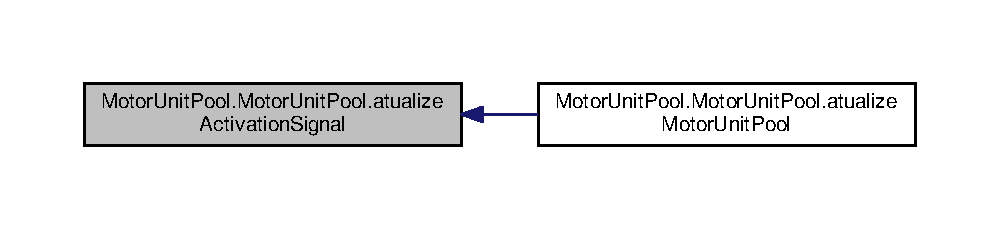
\includegraphics[width=350pt]{class_motor_unit_pool_1_1_motor_unit_pool_a03b7c1202f680bd8ba3af9b0b06bd71c_icgraph}
\end{center}
\end{figure}


\hypertarget{class_motor_unit_pool_1_1_motor_unit_pool_a8fbb182559fe08eb45800271655b711f}{\index{Motor\-Unit\-Pool\-::\-Motor\-Unit\-Pool@{Motor\-Unit\-Pool\-::\-Motor\-Unit\-Pool}!atualize\-Force\-No\-Hill@{atualize\-Force\-No\-Hill}}
\index{atualize\-Force\-No\-Hill@{atualize\-Force\-No\-Hill}!MotorUnitPool::MotorUnitPool@{Motor\-Unit\-Pool\-::\-Motor\-Unit\-Pool}}
\subsubsection[{atualize\-Force\-No\-Hill}]{\setlength{\rightskip}{0pt plus 5cm}def Motor\-Unit\-Pool.\-Motor\-Unit\-Pool.\-atualize\-Force\-No\-Hill (
\begin{DoxyParamCaption}
\item[{}]{self}
\end{DoxyParamCaption}
)}}\label{class_motor_unit_pool_1_1_motor_unit_pool_a8fbb182559fe08eb45800271655b711f}


Compute the muscle force when no muscle dynamics (Hill model) is used. 



Definition at line 152 of file Motor\-Unit\-Pool.\-py.

\hypertarget{class_motor_unit_pool_1_1_motor_unit_pool_ae525c6bba27837f09d2a767544780b0f}{\index{Motor\-Unit\-Pool\-::\-Motor\-Unit\-Pool@{Motor\-Unit\-Pool\-::\-Motor\-Unit\-Pool}!atualize\-Motor\-Unit\-Pool@{atualize\-Motor\-Unit\-Pool}}
\index{atualize\-Motor\-Unit\-Pool@{atualize\-Motor\-Unit\-Pool}!MotorUnitPool::MotorUnitPool@{Motor\-Unit\-Pool\-::\-Motor\-Unit\-Pool}}
\subsubsection[{atualize\-Motor\-Unit\-Pool}]{\setlength{\rightskip}{0pt plus 5cm}def Motor\-Unit\-Pool.\-Motor\-Unit\-Pool.\-atualize\-Motor\-Unit\-Pool (
\begin{DoxyParamCaption}
\item[{}]{self, }
\item[{}]{t}
\end{DoxyParamCaption}
)}}\label{class_motor_unit_pool_1_1_motor_unit_pool_ae525c6bba27837f09d2a767544780b0f}


Definition at line 129 of file Motor\-Unit\-Pool.\-py.



Here is the call graph for this function\-:\nopagebreak
\begin{figure}[H]
\begin{center}
\leavevmode
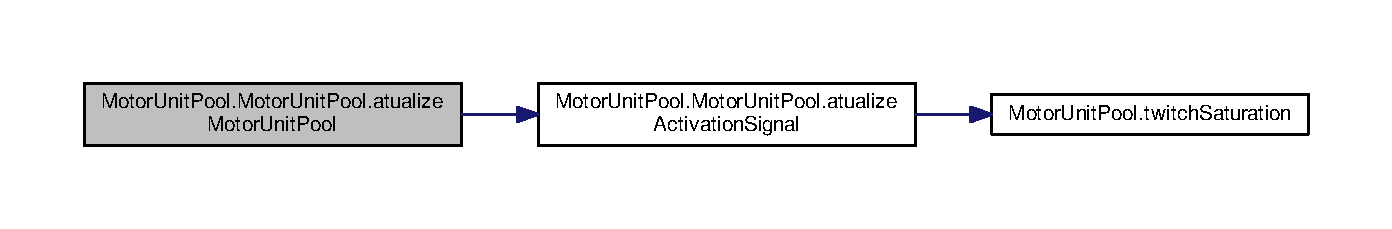
\includegraphics[width=350pt]{class_motor_unit_pool_1_1_motor_unit_pool_ae525c6bba27837f09d2a767544780b0f_cgraph}
\end{center}
\end{figure}


\hypertarget{class_motor_unit_pool_1_1_motor_unit_pool_a156ffc40be4c7c37f79905fa58b017e5}{\index{Motor\-Unit\-Pool\-::\-Motor\-Unit\-Pool@{Motor\-Unit\-Pool\-::\-Motor\-Unit\-Pool}!list\-Spikes@{list\-Spikes}}
\index{list\-Spikes@{list\-Spikes}!MotorUnitPool::MotorUnitPool@{Motor\-Unit\-Pool\-::\-Motor\-Unit\-Pool}}
\subsubsection[{list\-Spikes}]{\setlength{\rightskip}{0pt plus 5cm}def Motor\-Unit\-Pool.\-Motor\-Unit\-Pool.\-list\-Spikes (
\begin{DoxyParamCaption}
\item[{}]{self}
\end{DoxyParamCaption}
)}}\label{class_motor_unit_pool_1_1_motor_unit_pool_a156ffc40be4c7c37f79905fa58b017e5}


Definition at line 157 of file Motor\-Unit\-Pool.\-py.



\subsection{Member Data Documentation}
\hypertarget{class_motor_unit_pool_1_1_motor_unit_pool_a467ac7b080b79b9515d5846d75e95d1c}{\index{Motor\-Unit\-Pool\-::\-Motor\-Unit\-Pool@{Motor\-Unit\-Pool\-::\-Motor\-Unit\-Pool}!activation\-\_\-non\-Sat@{activation\-\_\-non\-Sat}}
\index{activation\-\_\-non\-Sat@{activation\-\_\-non\-Sat}!MotorUnitPool::MotorUnitPool@{Motor\-Unit\-Pool\-::\-Motor\-Unit\-Pool}}
\subsubsection[{activation\-\_\-non\-Sat}]{\setlength{\rightskip}{0pt plus 5cm}Motor\-Unit\-Pool.\-Motor\-Unit\-Pool.\-activation\-\_\-non\-Sat}}\label{class_motor_unit_pool_1_1_motor_unit_pool_a467ac7b080b79b9515d5846d75e95d1c}


Definition at line 105 of file Motor\-Unit\-Pool.\-py.

\hypertarget{class_motor_unit_pool_1_1_motor_unit_pool_ac475d1369c38d0bc5064c7243b4e1d44}{\index{Motor\-Unit\-Pool\-::\-Motor\-Unit\-Pool@{Motor\-Unit\-Pool\-::\-Motor\-Unit\-Pool}!activation\-\_\-\-Sat@{activation\-\_\-\-Sat}}
\index{activation\-\_\-\-Sat@{activation\-\_\-\-Sat}!MotorUnitPool::MotorUnitPool@{Motor\-Unit\-Pool\-::\-Motor\-Unit\-Pool}}
\subsubsection[{activation\-\_\-\-Sat}]{\setlength{\rightskip}{0pt plus 5cm}Motor\-Unit\-Pool.\-Motor\-Unit\-Pool.\-activation\-\_\-\-Sat}}\label{class_motor_unit_pool_1_1_motor_unit_pool_ac475d1369c38d0bc5064c7243b4e1d44}


Definition at line 114 of file Motor\-Unit\-Pool.\-py.

\hypertarget{class_motor_unit_pool_1_1_motor_unit_pool_abaa7680d0691fac81f66b200dfcfd203}{\index{Motor\-Unit\-Pool\-::\-Motor\-Unit\-Pool@{Motor\-Unit\-Pool\-::\-Motor\-Unit\-Pool}!activation\-Model@{activation\-Model}}
\index{activation\-Model@{activation\-Model}!MotorUnitPool::MotorUnitPool@{Motor\-Unit\-Pool\-::\-Motor\-Unit\-Pool}}
\subsubsection[{activation\-Model}]{\setlength{\rightskip}{0pt plus 5cm}Motor\-Unit\-Pool.\-Motor\-Unit\-Pool.\-activation\-Model}}\label{class_motor_unit_pool_1_1_motor_unit_pool_abaa7680d0691fac81f66b200dfcfd203}


Model of the activation signal. 

For now, it can be {\itshape S\-O\-C\-D\-S} (second order critically damped system). 

Definition at line 86 of file Motor\-Unit\-Pool.\-py.

\hypertarget{class_motor_unit_pool_1_1_motor_unit_pool_ad03b9e215e833188060e90bc4392d42b}{\index{Motor\-Unit\-Pool\-::\-Motor\-Unit\-Pool@{Motor\-Unit\-Pool\-::\-Motor\-Unit\-Pool}!Act\-Matrix@{Act\-Matrix}}
\index{Act\-Matrix@{Act\-Matrix}!MotorUnitPool::MotorUnitPool@{Motor\-Unit\-Pool\-::\-Motor\-Unit\-Pool}}
\subsubsection[{Act\-Matrix}]{\setlength{\rightskip}{0pt plus 5cm}Motor\-Unit\-Pool.\-Motor\-Unit\-Pool.\-Act\-Matrix}}\label{class_motor_unit_pool_1_1_motor_unit_pool_ad03b9e215e833188060e90bc4392d42b}


Definition at line 94 of file Motor\-Unit\-Pool.\-py.

\hypertarget{class_motor_unit_pool_1_1_motor_unit_pool_ac72c67b4a1f6134965ab77e2d798b5a4}{\index{Motor\-Unit\-Pool\-::\-Motor\-Unit\-Pool@{Motor\-Unit\-Pool\-::\-Motor\-Unit\-Pool}!an@{an}}
\index{an@{an}!MotorUnitPool::MotorUnitPool@{Motor\-Unit\-Pool\-::\-Motor\-Unit\-Pool}}
\subsubsection[{an}]{\setlength{\rightskip}{0pt plus 5cm}Motor\-Unit\-Pool.\-Motor\-Unit\-Pool.\-an}}\label{class_motor_unit_pool_1_1_motor_unit_pool_ac72c67b4a1f6134965ab77e2d798b5a4}


Definition at line 103 of file Motor\-Unit\-Pool.\-py.

\hypertarget{class_motor_unit_pool_1_1_motor_unit_pool_a21f9a6a5d113b5b0f67a3557c47ebd5a}{\index{Motor\-Unit\-Pool\-::\-Motor\-Unit\-Pool@{Motor\-Unit\-Pool\-::\-Motor\-Unit\-Pool}!atualize\-Force@{atualize\-Force}}
\index{atualize\-Force@{atualize\-Force}!MotorUnitPool::MotorUnitPool@{Motor\-Unit\-Pool\-::\-Motor\-Unit\-Pool}}
\subsubsection[{atualize\-Force}]{\setlength{\rightskip}{0pt plus 5cm}Motor\-Unit\-Pool.\-Motor\-Unit\-Pool.\-atualize\-Force}}\label{class_motor_unit_pool_1_1_motor_unit_pool_a21f9a6a5d113b5b0f67a3557c47ebd5a}


Definition at line 121 of file Motor\-Unit\-Pool.\-py.

\hypertarget{class_motor_unit_pool_1_1_motor_unit_pool_a4e107835e34b4f56d06b9b28c143fe40}{\index{Motor\-Unit\-Pool\-::\-Motor\-Unit\-Pool@{Motor\-Unit\-Pool\-::\-Motor\-Unit\-Pool}!b\-Sat@{b\-Sat}}
\index{b\-Sat@{b\-Sat}!MotorUnitPool::MotorUnitPool@{Motor\-Unit\-Pool\-::\-Motor\-Unit\-Pool}}
\subsubsection[{b\-Sat}]{\setlength{\rightskip}{0pt plus 5cm}Motor\-Unit\-Pool.\-Motor\-Unit\-Pool.\-b\-Sat}}\label{class_motor_unit_pool_1_1_motor_unit_pool_a4e107835e34b4f56d06b9b28c143fe40}


Definition at line 106 of file Motor\-Unit\-Pool.\-py.

\hypertarget{class_motor_unit_pool_1_1_motor_unit_pool_a3b2ee8f3e5500bfdc8fa731a5cb7d622}{\index{Motor\-Unit\-Pool\-::\-Motor\-Unit\-Pool@{Motor\-Unit\-Pool\-::\-Motor\-Unit\-Pool}!conf@{conf}}
\index{conf@{conf}!MotorUnitPool::MotorUnitPool@{Motor\-Unit\-Pool\-::\-Motor\-Unit\-Pool}}
\subsubsection[{conf}]{\setlength{\rightskip}{0pt plus 5cm}Motor\-Unit\-Pool.\-Motor\-Unit\-Pool.\-conf}}\label{class_motor_unit_pool_1_1_motor_unit_pool_a3b2ee8f3e5500bfdc8fa731a5cb7d622}


\hyperlink{namespace_configuration}{Configuration} object with the simulation parameters. 



Definition at line 58 of file Motor\-Unit\-Pool.\-py.

\hypertarget{class_motor_unit_pool_1_1_motor_unit_pool_a48b53d4f838ca8cfe2bc41c8308f2060}{\index{Motor\-Unit\-Pool\-::\-Motor\-Unit\-Pool@{Motor\-Unit\-Pool\-::\-Motor\-Unit\-Pool}!dirac\-Delta\-Value@{dirac\-Delta\-Value}}
\index{dirac\-Delta\-Value@{dirac\-Delta\-Value}!MotorUnitPool::MotorUnitPool@{Motor\-Unit\-Pool\-::\-Motor\-Unit\-Pool}}
\subsubsection[{dirac\-Delta\-Value}]{\setlength{\rightskip}{0pt plus 5cm}Motor\-Unit\-Pool.\-Motor\-Unit\-Pool.\-dirac\-Delta\-Value}}\label{class_motor_unit_pool_1_1_motor_unit_pool_a48b53d4f838ca8cfe2bc41c8308f2060}


Definition at line 116 of file Motor\-Unit\-Pool.\-py.

\hypertarget{class_motor_unit_pool_1_1_motor_unit_pool_a97011c17140c45a42a00105279f014ad}{\index{Motor\-Unit\-Pool\-::\-Motor\-Unit\-Pool@{Motor\-Unit\-Pool\-::\-Motor\-Unit\-Pool}!force@{force}}
\index{force@{force}!MotorUnitPool::MotorUnitPool@{Motor\-Unit\-Pool\-::\-Motor\-Unit\-Pool}}
\subsubsection[{force}]{\setlength{\rightskip}{0pt plus 5cm}Motor\-Unit\-Pool.\-Motor\-Unit\-Pool.\-force}}\label{class_motor_unit_pool_1_1_motor_unit_pool_a97011c17140c45a42a00105279f014ad}


Definition at line 119 of file Motor\-Unit\-Pool.\-py.

\hypertarget{class_motor_unit_pool_1_1_motor_unit_pool_a963061fdcfee8f9dc33e4d6f130ea59b}{\index{Motor\-Unit\-Pool\-::\-Motor\-Unit\-Pool@{Motor\-Unit\-Pool\-::\-Motor\-Unit\-Pool}!hill\-Model@{hill\-Model}}
\index{hill\-Model@{hill\-Model}!MotorUnitPool::MotorUnitPool@{Motor\-Unit\-Pool\-::\-Motor\-Unit\-Pool}}
\subsubsection[{hill\-Model}]{\setlength{\rightskip}{0pt plus 5cm}Motor\-Unit\-Pool.\-Motor\-Unit\-Pool.\-hill\-Model}}\label{class_motor_unit_pool_1_1_motor_unit_pool_a963061fdcfee8f9dc33e4d6f130ea59b}


Definition at line 120 of file Motor\-Unit\-Pool.\-py.

\hypertarget{class_motor_unit_pool_1_1_motor_unit_pool_aeb57d0463ad56a16b166d00dc6079b95}{\index{Motor\-Unit\-Pool\-::\-Motor\-Unit\-Pool@{Motor\-Unit\-Pool\-::\-Motor\-Unit\-Pool}!kind@{kind}}
\index{kind@{kind}!MotorUnitPool::MotorUnitPool@{Motor\-Unit\-Pool\-::\-Motor\-Unit\-Pool}}
\subsubsection[{kind}]{\setlength{\rightskip}{0pt plus 5cm}Motor\-Unit\-Pool.\-Motor\-Unit\-Pool.\-kind}}\label{class_motor_unit_pool_1_1_motor_unit_pool_aeb57d0463ad56a16b166d00dc6079b95}


Indicates that is Motor Unit pool. 



Definition at line 55 of file Motor\-Unit\-Pool.\-py.

\hypertarget{class_motor_unit_pool_1_1_motor_unit_pool_aa5884530baaa20f46007805bc574407d}{\index{Motor\-Unit\-Pool\-::\-Motor\-Unit\-Pool@{Motor\-Unit\-Pool\-::\-Motor\-Unit\-Pool}!M\-Unumber@{M\-Unumber}}
\index{M\-Unumber@{M\-Unumber}!MotorUnitPool::MotorUnitPool@{Motor\-Unit\-Pool\-::\-Motor\-Unit\-Pool}}
\subsubsection[{M\-Unumber}]{\setlength{\rightskip}{0pt plus 5cm}Motor\-Unit\-Pool.\-Motor\-Unit\-Pool.\-M\-Unumber}}\label{class_motor_unit_pool_1_1_motor_unit_pool_aa5884530baaa20f46007805bc574407d}


Number of motor units. 



Definition at line 65 of file Motor\-Unit\-Pool.\-py.

\hypertarget{class_motor_unit_pool_1_1_motor_unit_pool_a832364dc014aa8a1b2947abfe063f626}{\index{Motor\-Unit\-Pool\-::\-Motor\-Unit\-Pool@{Motor\-Unit\-Pool\-::\-Motor\-Unit\-Pool}!pool@{pool}}
\index{pool@{pool}!MotorUnitPool::MotorUnitPool@{Motor\-Unit\-Pool\-::\-Motor\-Unit\-Pool}}
\subsubsection[{pool}]{\setlength{\rightskip}{0pt plus 5cm}Motor\-Unit\-Pool.\-Motor\-Unit\-Pool.\-pool}}\label{class_motor_unit_pool_1_1_motor_unit_pool_a832364dc014aa8a1b2947abfe063f626}


String with Motor unit pool to which the motor unit belongs. 



Definition at line 60 of file Motor\-Unit\-Pool.\-py.

\hypertarget{class_motor_unit_pool_1_1_motor_unit_pool_a3790757a111061662ad0f98120b25e69}{\index{Motor\-Unit\-Pool\-::\-Motor\-Unit\-Pool@{Motor\-Unit\-Pool\-::\-Motor\-Unit\-Pool}!pool\-Soma\-Spikes@{pool\-Soma\-Spikes}}
\index{pool\-Soma\-Spikes@{pool\-Soma\-Spikes}!MotorUnitPool::MotorUnitPool@{Motor\-Unit\-Pool\-::\-Motor\-Unit\-Pool}}
\subsubsection[{pool\-Soma\-Spikes}]{\setlength{\rightskip}{0pt plus 5cm}Motor\-Unit\-Pool.\-Motor\-Unit\-Pool.\-pool\-Soma\-Spikes}}\label{class_motor_unit_pool_1_1_motor_unit_pool_a3790757a111061662ad0f98120b25e69}


Vector with the instants of spikes in the soma compartment, in ms. 



Definition at line 80 of file Motor\-Unit\-Pool.\-py.

\hypertarget{class_motor_unit_pool_1_1_motor_unit_pool_a4f0b93df27eb6303fa1a3d49653d4fd3}{\index{Motor\-Unit\-Pool\-::\-Motor\-Unit\-Pool@{Motor\-Unit\-Pool\-::\-Motor\-Unit\-Pool}!pool\-Terminal\-Spikes@{pool\-Terminal\-Spikes}}
\index{pool\-Terminal\-Spikes@{pool\-Terminal\-Spikes}!MotorUnitPool::MotorUnitPool@{Motor\-Unit\-Pool\-::\-Motor\-Unit\-Pool}}
\subsubsection[{pool\-Terminal\-Spikes}]{\setlength{\rightskip}{0pt plus 5cm}Motor\-Unit\-Pool.\-Motor\-Unit\-Pool.\-pool\-Terminal\-Spikes}}\label{class_motor_unit_pool_1_1_motor_unit_pool_a4f0b93df27eb6303fa1a3d49653d4fd3}


Vector with the instants of spikes in the terminal, in ms. 



Definition at line 82 of file Motor\-Unit\-Pool.\-py.

\hypertarget{class_motor_unit_pool_1_1_motor_unit_pool_ab5659e1c9355ecf529d9b8be8cbf6d65}{\index{Motor\-Unit\-Pool\-::\-Motor\-Unit\-Pool@{Motor\-Unit\-Pool\-::\-Motor\-Unit\-Pool}!time\-Index@{time\-Index}}
\index{time\-Index@{time\-Index}!MotorUnitPool::MotorUnitPool@{Motor\-Unit\-Pool\-::\-Motor\-Unit\-Pool}}
\subsubsection[{time\-Index}]{\setlength{\rightskip}{0pt plus 5cm}Motor\-Unit\-Pool.\-Motor\-Unit\-Pool.\-time\-Index}}\label{class_motor_unit_pool_1_1_motor_unit_pool_ab5659e1c9355ecf529d9b8be8cbf6d65}


Definition at line 123 of file Motor\-Unit\-Pool.\-py.

\hypertarget{class_motor_unit_pool_1_1_motor_unit_pool_a03538b06e7220f9d48c7306ed6508c05}{\index{Motor\-Unit\-Pool\-::\-Motor\-Unit\-Pool@{Motor\-Unit\-Pool\-::\-Motor\-Unit\-Pool}!twitch\-Amp\-\_\-\-N@{twitch\-Amp\-\_\-\-N}}
\index{twitch\-Amp\-\_\-\-N@{twitch\-Amp\-\_\-\-N}!MotorUnitPool::MotorUnitPool@{Motor\-Unit\-Pool\-::\-Motor\-Unit\-Pool}}
\subsubsection[{twitch\-Amp\-\_\-\-N}]{\setlength{\rightskip}{0pt plus 5cm}Motor\-Unit\-Pool.\-Motor\-Unit\-Pool.\-twitch\-Amp\-\_\-\-N}}\label{class_motor_unit_pool_1_1_motor_unit_pool_a03538b06e7220f9d48c7306ed6508c05}


Definition at line 108 of file Motor\-Unit\-Pool.\-py.

\hypertarget{class_motor_unit_pool_1_1_motor_unit_pool_a785a769c5b4824603a24339e4f0d8dfe}{\index{Motor\-Unit\-Pool\-::\-Motor\-Unit\-Pool@{Motor\-Unit\-Pool\-::\-Motor\-Unit\-Pool}!tw\-Tet@{tw\-Tet}}
\index{tw\-Tet@{tw\-Tet}!MotorUnitPool::MotorUnitPool@{Motor\-Unit\-Pool\-::\-Motor\-Unit\-Pool}}
\subsubsection[{tw\-Tet}]{\setlength{\rightskip}{0pt plus 5cm}Motor\-Unit\-Pool.\-Motor\-Unit\-Pool.\-tw\-Tet}}\label{class_motor_unit_pool_1_1_motor_unit_pool_a785a769c5b4824603a24339e4f0d8dfe}


Definition at line 107 of file Motor\-Unit\-Pool.\-py.

\hypertarget{class_motor_unit_pool_1_1_motor_unit_pool_a1b14c831606c27efae62f1468850393b}{\index{Motor\-Unit\-Pool\-::\-Motor\-Unit\-Pool@{Motor\-Unit\-Pool\-::\-Motor\-Unit\-Pool}!unit@{unit}}
\index{unit@{unit}!MotorUnitPool::MotorUnitPool@{Motor\-Unit\-Pool\-::\-Motor\-Unit\-Pool}}
\subsubsection[{unit}]{\setlength{\rightskip}{0pt plus 5cm}Motor\-Unit\-Pool.\-Motor\-Unit\-Pool.\-unit}}\label{class_motor_unit_pool_1_1_motor_unit_pool_a1b14c831606c27efae62f1468850393b}


List of \hyperlink{namespace_motor_unit}{Motor\-Unit} objects. 



Definition at line 68 of file Motor\-Unit\-Pool.\-py.



The documentation for this class was generated from the following file\-:\begin{DoxyCompactItemize}
\item 
\hyperlink{_motor_unit_pool_8py}{Motor\-Unit\-Pool.\-py}\end{DoxyCompactItemize}

\hypertarget{class_neural_tract_1_1_neural_tract}{\section{Neural\-Tract.\-Neural\-Tract Class Reference}
\label{class_neural_tract_1_1_neural_tract}\index{Neural\-Tract.\-Neural\-Tract@{Neural\-Tract.\-Neural\-Tract}}
}


classdocs  


\subsection*{Public Member Functions}
\begin{DoxyCompactItemize}
\item 
def \hyperlink{class_neural_tract_1_1_neural_tract_a4bcd77ff91855685b0b96d3522ba7d20}{\-\_\-\-\_\-init\-\_\-\-\_\-}
\begin{DoxyCompactList}\small\item\em Constructor. \end{DoxyCompactList}\item 
def \hyperlink{class_neural_tract_1_1_neural_tract_a0f826ea8fadc13ea0af3bfdf5508b4f0}{atualize\-Pool}
\item 
def \hyperlink{class_neural_tract_1_1_neural_tract_a600b048655026f9271cec0a812b11dc4}{list\-Spikes}
\end{DoxyCompactItemize}
\subsection*{Public Attributes}
\begin{DoxyCompactItemize}
\item 
\hyperlink{class_neural_tract_1_1_neural_tract_af52b112c86e0c774fa204b7e2154b6aa}{kind}
\item 
\hyperlink{class_neural_tract_1_1_neural_tract_af0d232b9b86f3bae802b32777d0405d0}{pool}
\item 
\hyperlink{class_neural_tract_1_1_neural_tract_a9cf4c6df3fb8818e955817bb3ea9ffc4}{Number}
\item 
\hyperlink{class_neural_tract_1_1_neural_tract_a95db7d0720ec12f091758968476ba240}{unit}
\item 
\hyperlink{class_neural_tract_1_1_neural_tract_a1d104906ff30028e44e377a9e1ed5a3d}{pool\-Terminal\-Spikes}
\item 
\hyperlink{class_neural_tract_1_1_neural_tract_a637995fcac5bdd80ab1a9d4ea3de7f40}{target}
\item 
\hyperlink{class_neural_tract_1_1_neural_tract_aefbec14cba88a937841314d47f6056c0}{F\-R}
\item 
\hyperlink{class_neural_tract_1_1_neural_tract_adcda2b95aa86d4e7eebcc2557aee58cf}{time\-Index}
\end{DoxyCompactItemize}


\subsection{Detailed Description}
classdocs 

Definition at line 14 of file Neural\-Tract.\-py.



\subsection{Constructor \& Destructor Documentation}
\hypertarget{class_neural_tract_1_1_neural_tract_a4bcd77ff91855685b0b96d3522ba7d20}{\index{Neural\-Tract\-::\-Neural\-Tract@{Neural\-Tract\-::\-Neural\-Tract}!\-\_\-\-\_\-init\-\_\-\-\_\-@{\-\_\-\-\_\-init\-\_\-\-\_\-}}
\index{\-\_\-\-\_\-init\-\_\-\-\_\-@{\-\_\-\-\_\-init\-\_\-\-\_\-}!NeuralTract::NeuralTract@{Neural\-Tract\-::\-Neural\-Tract}}
\subsubsection[{\-\_\-\-\_\-init\-\_\-\-\_\-}]{\setlength{\rightskip}{0pt plus 5cm}def Neural\-Tract.\-Neural\-Tract.\-\_\-\-\_\-init\-\_\-\-\_\- (
\begin{DoxyParamCaption}
\item[{}]{self, }
\item[{}]{conf, }
\item[{}]{pool}
\end{DoxyParamCaption}
)}}\label{class_neural_tract_1_1_neural_tract_a4bcd77ff91855685b0b96d3522ba7d20}


Constructor. 


\begin{DoxyItemize}
\item Inputs\-:
\begin{DoxyItemize}
\item {\bfseries conf}\-:
\item {\bfseries pool}\-: 
\end{DoxyItemize}
\end{DoxyItemize}

Definition at line 26 of file Neural\-Tract.\-py.



\subsection{Member Function Documentation}
\hypertarget{class_neural_tract_1_1_neural_tract_a0f826ea8fadc13ea0af3bfdf5508b4f0}{\index{Neural\-Tract\-::\-Neural\-Tract@{Neural\-Tract\-::\-Neural\-Tract}!atualize\-Pool@{atualize\-Pool}}
\index{atualize\-Pool@{atualize\-Pool}!NeuralTract::NeuralTract@{Neural\-Tract\-::\-Neural\-Tract}}
\subsubsection[{atualize\-Pool}]{\setlength{\rightskip}{0pt plus 5cm}def Neural\-Tract.\-Neural\-Tract.\-atualize\-Pool (
\begin{DoxyParamCaption}
\item[{}]{self, }
\item[{}]{t}
\end{DoxyParamCaption}
)}}\label{class_neural_tract_1_1_neural_tract_a0f826ea8fadc13ea0af3bfdf5508b4f0}


Definition at line 50 of file Neural\-Tract.\-py.

\hypertarget{class_neural_tract_1_1_neural_tract_a600b048655026f9271cec0a812b11dc4}{\index{Neural\-Tract\-::\-Neural\-Tract@{Neural\-Tract\-::\-Neural\-Tract}!list\-Spikes@{list\-Spikes}}
\index{list\-Spikes@{list\-Spikes}!NeuralTract::NeuralTract@{Neural\-Tract\-::\-Neural\-Tract}}
\subsubsection[{list\-Spikes}]{\setlength{\rightskip}{0pt plus 5cm}def Neural\-Tract.\-Neural\-Tract.\-list\-Spikes (
\begin{DoxyParamCaption}
\item[{}]{self}
\end{DoxyParamCaption}
)}}\label{class_neural_tract_1_1_neural_tract_a600b048655026f9271cec0a812b11dc4}


Definition at line 55 of file Neural\-Tract.\-py.



\subsection{Member Data Documentation}
\hypertarget{class_neural_tract_1_1_neural_tract_aefbec14cba88a937841314d47f6056c0}{\index{Neural\-Tract\-::\-Neural\-Tract@{Neural\-Tract\-::\-Neural\-Tract}!F\-R@{F\-R}}
\index{F\-R@{F\-R}!NeuralTract::NeuralTract@{Neural\-Tract\-::\-Neural\-Tract}}
\subsubsection[{F\-R}]{\setlength{\rightskip}{0pt plus 5cm}Neural\-Tract.\-Neural\-Tract.\-F\-R}}\label{class_neural_tract_1_1_neural_tract_aefbec14cba88a937841314d47f6056c0}


Definition at line 43 of file Neural\-Tract.\-py.

\hypertarget{class_neural_tract_1_1_neural_tract_af52b112c86e0c774fa204b7e2154b6aa}{\index{Neural\-Tract\-::\-Neural\-Tract@{Neural\-Tract\-::\-Neural\-Tract}!kind@{kind}}
\index{kind@{kind}!NeuralTract::NeuralTract@{Neural\-Tract\-::\-Neural\-Tract}}
\subsubsection[{kind}]{\setlength{\rightskip}{0pt plus 5cm}Neural\-Tract.\-Neural\-Tract.\-kind}}\label{class_neural_tract_1_1_neural_tract_af52b112c86e0c774fa204b7e2154b6aa}


Definition at line 27 of file Neural\-Tract.\-py.

\hypertarget{class_neural_tract_1_1_neural_tract_a9cf4c6df3fb8818e955817bb3ea9ffc4}{\index{Neural\-Tract\-::\-Neural\-Tract@{Neural\-Tract\-::\-Neural\-Tract}!Number@{Number}}
\index{Number@{Number}!NeuralTract::NeuralTract@{Neural\-Tract\-::\-Neural\-Tract}}
\subsubsection[{Number}]{\setlength{\rightskip}{0pt plus 5cm}Neural\-Tract.\-Neural\-Tract.\-Number}}\label{class_neural_tract_1_1_neural_tract_a9cf4c6df3fb8818e955817bb3ea9ffc4}


Definition at line 29 of file Neural\-Tract.\-py.

\hypertarget{class_neural_tract_1_1_neural_tract_af0d232b9b86f3bae802b32777d0405d0}{\index{Neural\-Tract\-::\-Neural\-Tract@{Neural\-Tract\-::\-Neural\-Tract}!pool@{pool}}
\index{pool@{pool}!NeuralTract::NeuralTract@{Neural\-Tract\-::\-Neural\-Tract}}
\subsubsection[{pool}]{\setlength{\rightskip}{0pt plus 5cm}Neural\-Tract.\-Neural\-Tract.\-pool}}\label{class_neural_tract_1_1_neural_tract_af0d232b9b86f3bae802b32777d0405d0}


Definition at line 28 of file Neural\-Tract.\-py.

\hypertarget{class_neural_tract_1_1_neural_tract_a1d104906ff30028e44e377a9e1ed5a3d}{\index{Neural\-Tract\-::\-Neural\-Tract@{Neural\-Tract\-::\-Neural\-Tract}!pool\-Terminal\-Spikes@{pool\-Terminal\-Spikes}}
\index{pool\-Terminal\-Spikes@{pool\-Terminal\-Spikes}!NeuralTract::NeuralTract@{Neural\-Tract\-::\-Neural\-Tract}}
\subsubsection[{pool\-Terminal\-Spikes}]{\setlength{\rightskip}{0pt plus 5cm}Neural\-Tract.\-Neural\-Tract.\-pool\-Terminal\-Spikes}}\label{class_neural_tract_1_1_neural_tract_a1d104906ff30028e44e377a9e1ed5a3d}


Definition at line 34 of file Neural\-Tract.\-py.

\hypertarget{class_neural_tract_1_1_neural_tract_a637995fcac5bdd80ab1a9d4ea3de7f40}{\index{Neural\-Tract\-::\-Neural\-Tract@{Neural\-Tract\-::\-Neural\-Tract}!target@{target}}
\index{target@{target}!NeuralTract::NeuralTract@{Neural\-Tract\-::\-Neural\-Tract}}
\subsubsection[{target}]{\setlength{\rightskip}{0pt plus 5cm}Neural\-Tract.\-Neural\-Tract.\-target}}\label{class_neural_tract_1_1_neural_tract_a637995fcac5bdd80ab1a9d4ea3de7f40}


Definition at line 36 of file Neural\-Tract.\-py.

\hypertarget{class_neural_tract_1_1_neural_tract_adcda2b95aa86d4e7eebcc2557aee58cf}{\index{Neural\-Tract\-::\-Neural\-Tract@{Neural\-Tract\-::\-Neural\-Tract}!time\-Index@{time\-Index}}
\index{time\-Index@{time\-Index}!NeuralTract::NeuralTract@{Neural\-Tract\-::\-Neural\-Tract}}
\subsubsection[{time\-Index}]{\setlength{\rightskip}{0pt plus 5cm}Neural\-Tract.\-Neural\-Tract.\-time\-Index}}\label{class_neural_tract_1_1_neural_tract_adcda2b95aa86d4e7eebcc2557aee58cf}


Definition at line 46 of file Neural\-Tract.\-py.

\hypertarget{class_neural_tract_1_1_neural_tract_a95db7d0720ec12f091758968476ba240}{\index{Neural\-Tract\-::\-Neural\-Tract@{Neural\-Tract\-::\-Neural\-Tract}!unit@{unit}}
\index{unit@{unit}!NeuralTract::NeuralTract@{Neural\-Tract\-::\-Neural\-Tract}}
\subsubsection[{unit}]{\setlength{\rightskip}{0pt plus 5cm}Neural\-Tract.\-Neural\-Tract.\-unit}}\label{class_neural_tract_1_1_neural_tract_a95db7d0720ec12f091758968476ba240}


Definition at line 31 of file Neural\-Tract.\-py.



The documentation for this class was generated from the following file\-:\begin{DoxyCompactItemize}
\item 
\hyperlink{_neural_tract_8py}{Neural\-Tract.\-py}\end{DoxyCompactItemize}

\hypertarget{class_neural_tract_unit_1_1_neural_tract_unit}{\section{Neural\-Tract\-Unit.\-Neural\-Tract\-Unit Class Reference}
\label{class_neural_tract_unit_1_1_neural_tract_unit}\index{Neural\-Tract\-Unit.\-Neural\-Tract\-Unit@{Neural\-Tract\-Unit.\-Neural\-Tract\-Unit}}
}


classdocs  


\subsection*{Public Member Functions}
\begin{DoxyCompactItemize}
\item 
def \hyperlink{class_neural_tract_unit_1_1_neural_tract_unit_a8b10daafc9b7e804ba7d1c62aa854fa6}{\-\_\-\-\_\-init\-\_\-\-\_\-}
\begin{DoxyCompactList}\small\item\em Constructor. \end{DoxyCompactList}\item 
def \hyperlink{class_neural_tract_unit_1_1_neural_tract_unit_aaa36d43c7f4d1664696922e731f9e14a}{atualize\-Neural\-Tract\-Unit}
\item 
def \hyperlink{class_neural_tract_unit_1_1_neural_tract_unit_a1c44e3b23ebda745d84d88c015c1cb25}{transmit\-Spikes}
\end{DoxyCompactItemize}
\subsection*{Public Attributes}
\begin{DoxyCompactItemize}
\item 
\hyperlink{class_neural_tract_unit_1_1_neural_tract_unit_aee01a134ce97127783d75757ec15f352}{Gamma\-Order}
\item 
\hyperlink{class_neural_tract_unit_1_1_neural_tract_unit_a57cbb130e004fb3f7ee8d8a540f7dff0}{spikes\-Generator}
\item 
\hyperlink{class_neural_tract_unit_1_1_neural_tract_unit_ac34c86235329e753e8cfdfcc1e24c53f}{terminal\-Spike\-Train}
\item 
\hyperlink{class_neural_tract_unit_1_1_neural_tract_unit_a740d2cfa17ad57c7dbd40fbafc654b95}{Synapses\-Out}
\item 
\hyperlink{class_neural_tract_unit_1_1_neural_tract_unit_ac6fa367f6ada8045919674feaed4f6ad}{transmit\-Spikes\-Through\-Synapses}
\item 
\hyperlink{class_neural_tract_unit_1_1_neural_tract_unit_a4e5fa20e16e924e7f27a087e8f7a19a7}{indices\-Of\-Synapses\-On\-Target}
\end{DoxyCompactItemize}


\subsection{Detailed Description}
classdocs 

Definition at line 20 of file Neural\-Tract\-Unit.\-py.



\subsection{Constructor \& Destructor Documentation}
\hypertarget{class_neural_tract_unit_1_1_neural_tract_unit_a8b10daafc9b7e804ba7d1c62aa854fa6}{\index{Neural\-Tract\-Unit\-::\-Neural\-Tract\-Unit@{Neural\-Tract\-Unit\-::\-Neural\-Tract\-Unit}!\-\_\-\-\_\-init\-\_\-\-\_\-@{\-\_\-\-\_\-init\-\_\-\-\_\-}}
\index{\-\_\-\-\_\-init\-\_\-\-\_\-@{\-\_\-\-\_\-init\-\_\-\-\_\-}!NeuralTractUnit::NeuralTractUnit@{Neural\-Tract\-Unit\-::\-Neural\-Tract\-Unit}}
\subsubsection[{\-\_\-\-\_\-init\-\_\-\-\_\-}]{\setlength{\rightskip}{0pt plus 5cm}def Neural\-Tract\-Unit.\-Neural\-Tract\-Unit.\-\_\-\-\_\-init\-\_\-\-\_\- (
\begin{DoxyParamCaption}
\item[{}]{self, }
\item[{}]{conf, }
\item[{}]{pool, }
\item[{}]{index}
\end{DoxyParamCaption}
)}}\label{class_neural_tract_unit_1_1_neural_tract_unit_a8b10daafc9b7e804ba7d1c62aa854fa6}


Constructor. 



Definition at line 27 of file Neural\-Tract\-Unit.\-py.



\subsection{Member Function Documentation}
\hypertarget{class_neural_tract_unit_1_1_neural_tract_unit_aaa36d43c7f4d1664696922e731f9e14a}{\index{Neural\-Tract\-Unit\-::\-Neural\-Tract\-Unit@{Neural\-Tract\-Unit\-::\-Neural\-Tract\-Unit}!atualize\-Neural\-Tract\-Unit@{atualize\-Neural\-Tract\-Unit}}
\index{atualize\-Neural\-Tract\-Unit@{atualize\-Neural\-Tract\-Unit}!NeuralTractUnit::NeuralTractUnit@{Neural\-Tract\-Unit\-::\-Neural\-Tract\-Unit}}
\subsubsection[{atualize\-Neural\-Tract\-Unit}]{\setlength{\rightskip}{0pt plus 5cm}def Neural\-Tract\-Unit.\-Neural\-Tract\-Unit.\-atualize\-Neural\-Tract\-Unit (
\begin{DoxyParamCaption}
\item[{}]{self, }
\item[{}]{t, }
\item[{}]{F\-R}
\end{DoxyParamCaption}
)}}\label{class_neural_tract_unit_1_1_neural_tract_unit_aaa36d43c7f4d1664696922e731f9e14a}


Definition at line 49 of file Neural\-Tract\-Unit.\-py.



Here is the call graph for this function\-:\nopagebreak
\begin{figure}[H]
\begin{center}
\leavevmode
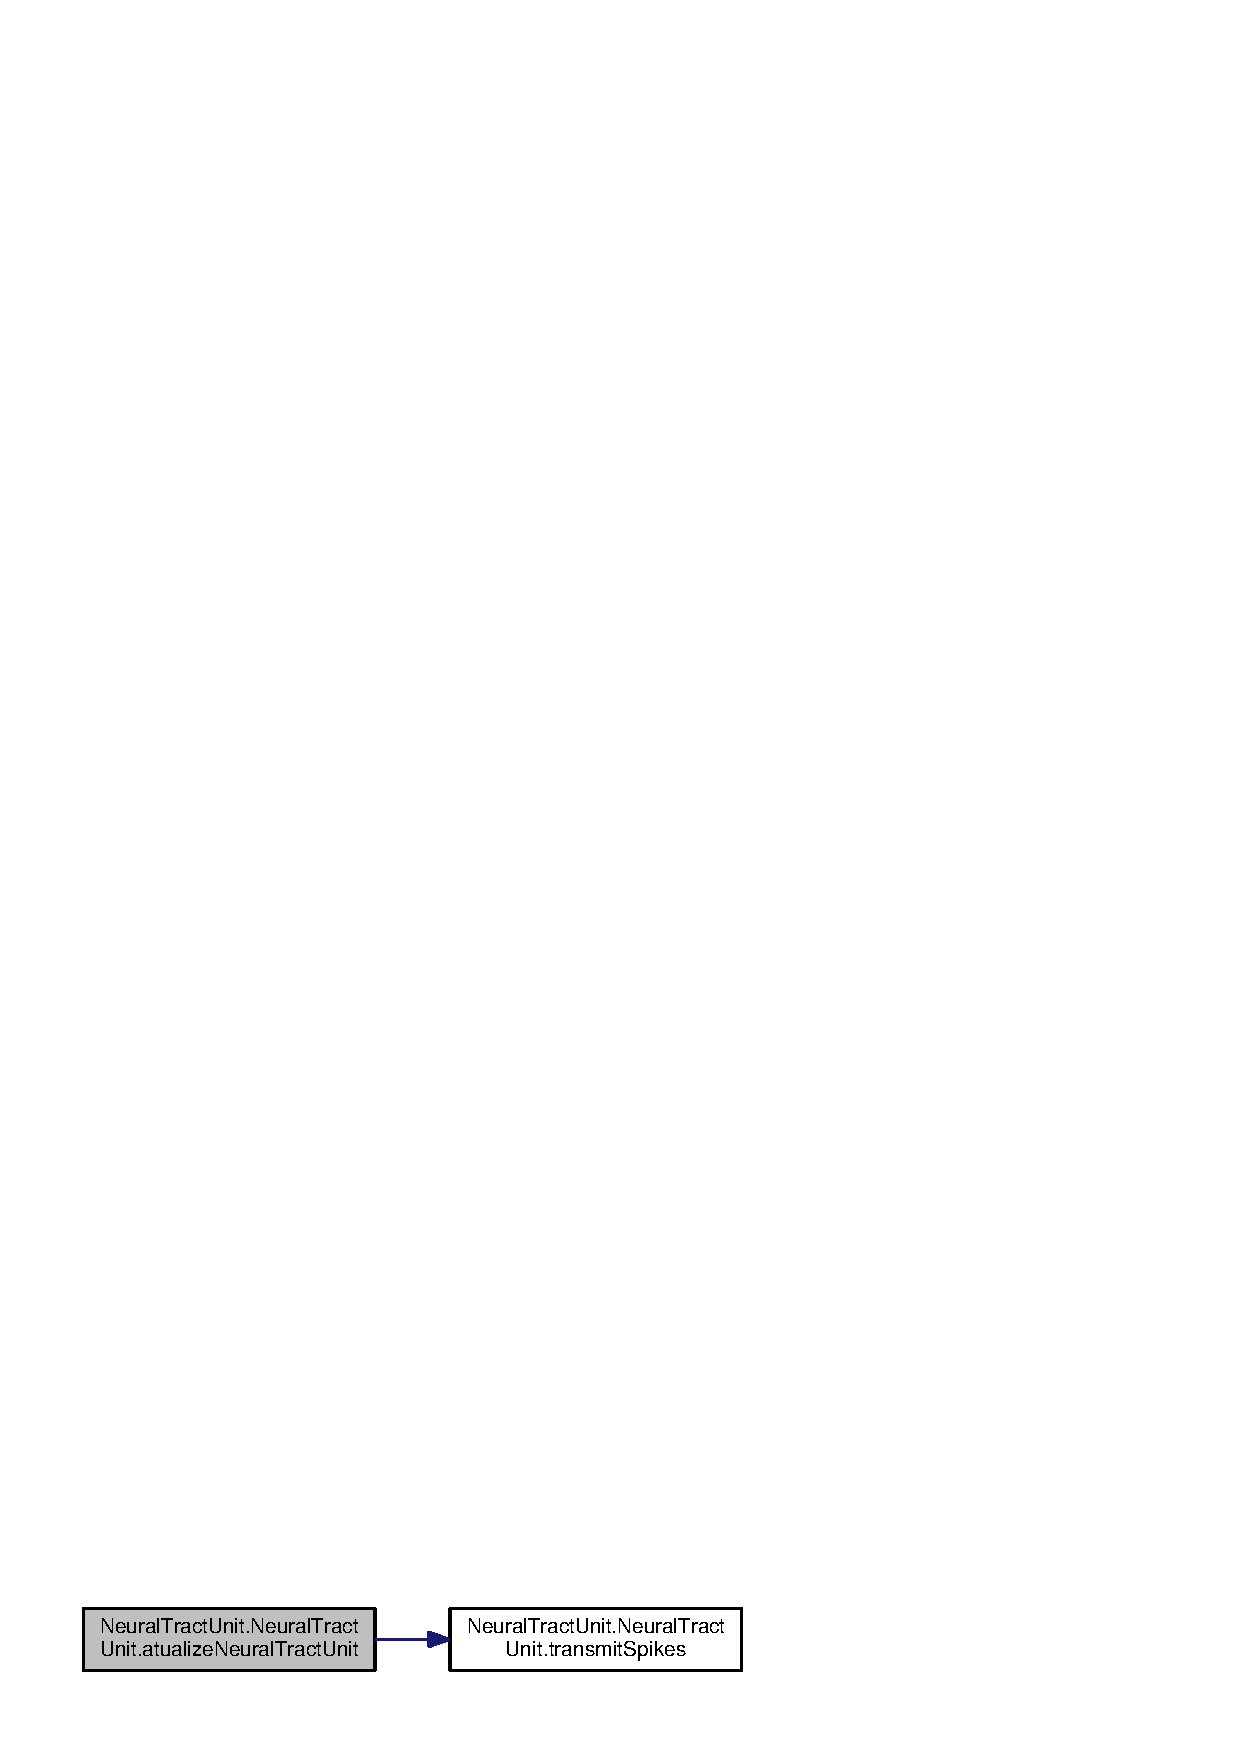
\includegraphics[width=350pt]{class_neural_tract_unit_1_1_neural_tract_unit_aaa36d43c7f4d1664696922e731f9e14a_cgraph}
\end{center}
\end{figure}


\hypertarget{class_neural_tract_unit_1_1_neural_tract_unit_a1c44e3b23ebda745d84d88c015c1cb25}{\index{Neural\-Tract\-Unit\-::\-Neural\-Tract\-Unit@{Neural\-Tract\-Unit\-::\-Neural\-Tract\-Unit}!transmit\-Spikes@{transmit\-Spikes}}
\index{transmit\-Spikes@{transmit\-Spikes}!NeuralTractUnit::NeuralTractUnit@{Neural\-Tract\-Unit\-::\-Neural\-Tract\-Unit}}
\subsubsection[{transmit\-Spikes}]{\setlength{\rightskip}{0pt plus 5cm}def Neural\-Tract\-Unit.\-Neural\-Tract\-Unit.\-transmit\-Spikes (
\begin{DoxyParamCaption}
\item[{}]{self, }
\item[{}]{t}
\end{DoxyParamCaption}
)}}\label{class_neural_tract_unit_1_1_neural_tract_unit_a1c44e3b23ebda745d84d88c015c1cb25}


Definition at line 59 of file Neural\-Tract\-Unit.\-py.



Here is the caller graph for this function\-:\nopagebreak
\begin{figure}[H]
\begin{center}
\leavevmode
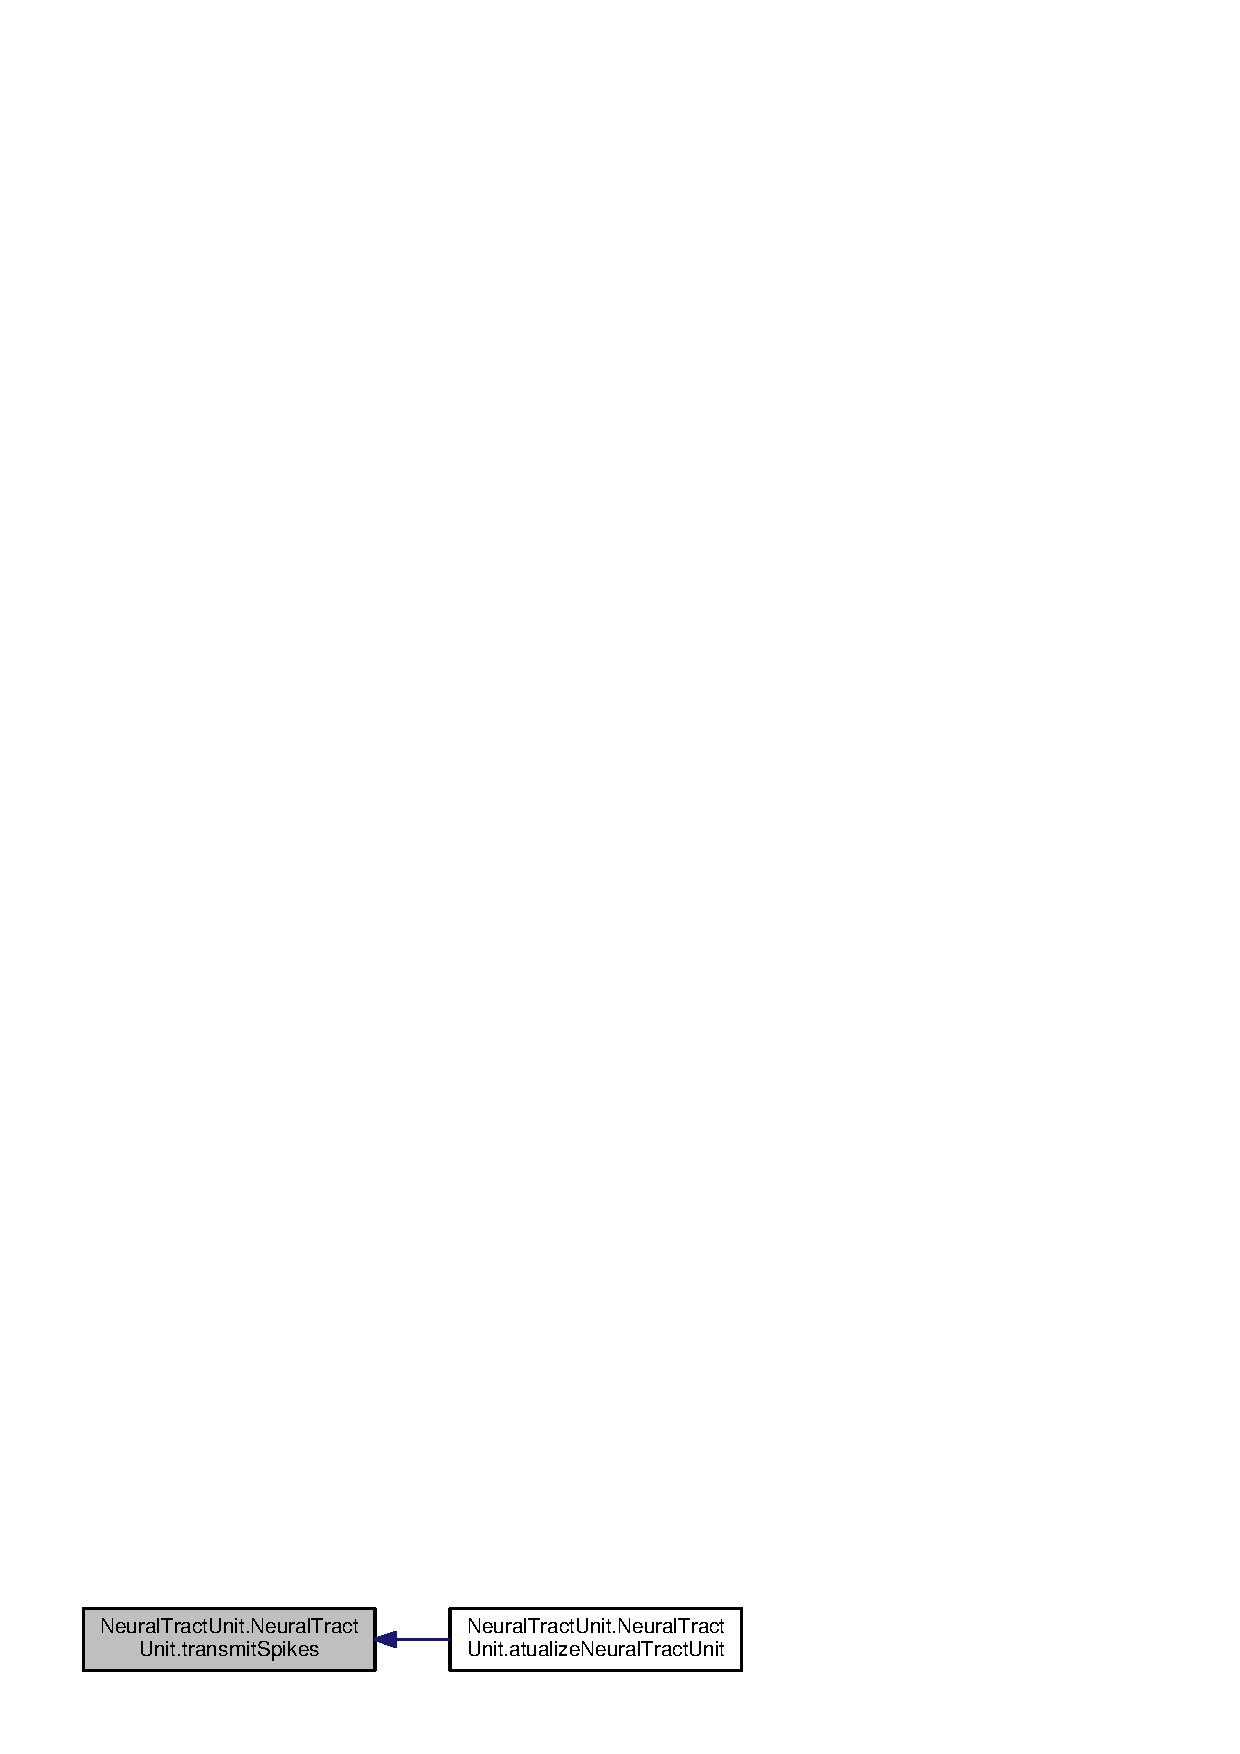
\includegraphics[width=350pt]{class_neural_tract_unit_1_1_neural_tract_unit_a1c44e3b23ebda745d84d88c015c1cb25_icgraph}
\end{center}
\end{figure}




\subsection{Member Data Documentation}
\hypertarget{class_neural_tract_unit_1_1_neural_tract_unit_aee01a134ce97127783d75757ec15f352}{\index{Neural\-Tract\-Unit\-::\-Neural\-Tract\-Unit@{Neural\-Tract\-Unit\-::\-Neural\-Tract\-Unit}!Gamma\-Order@{Gamma\-Order}}
\index{Gamma\-Order@{Gamma\-Order}!NeuralTractUnit::NeuralTractUnit@{Neural\-Tract\-Unit\-::\-Neural\-Tract\-Unit}}
\subsubsection[{Gamma\-Order}]{\setlength{\rightskip}{0pt plus 5cm}Neural\-Tract\-Unit.\-Neural\-Tract\-Unit.\-Gamma\-Order}}\label{class_neural_tract_unit_1_1_neural_tract_unit_aee01a134ce97127783d75757ec15f352}


Definition at line 29 of file Neural\-Tract\-Unit.\-py.

\hypertarget{class_neural_tract_unit_1_1_neural_tract_unit_a4e5fa20e16e924e7f27a087e8f7a19a7}{\index{Neural\-Tract\-Unit\-::\-Neural\-Tract\-Unit@{Neural\-Tract\-Unit\-::\-Neural\-Tract\-Unit}!indices\-Of\-Synapses\-On\-Target@{indices\-Of\-Synapses\-On\-Target}}
\index{indices\-Of\-Synapses\-On\-Target@{indices\-Of\-Synapses\-On\-Target}!NeuralTractUnit::NeuralTractUnit@{Neural\-Tract\-Unit\-::\-Neural\-Tract\-Unit}}
\subsubsection[{indices\-Of\-Synapses\-On\-Target}]{\setlength{\rightskip}{0pt plus 5cm}Neural\-Tract\-Unit.\-Neural\-Tract\-Unit.\-indices\-Of\-Synapses\-On\-Target}}\label{class_neural_tract_unit_1_1_neural_tract_unit_a4e5fa20e16e924e7f27a087e8f7a19a7}


Definition at line 41 of file Neural\-Tract\-Unit.\-py.

\hypertarget{class_neural_tract_unit_1_1_neural_tract_unit_a57cbb130e004fb3f7ee8d8a540f7dff0}{\index{Neural\-Tract\-Unit\-::\-Neural\-Tract\-Unit@{Neural\-Tract\-Unit\-::\-Neural\-Tract\-Unit}!spikes\-Generator@{spikes\-Generator}}
\index{spikes\-Generator@{spikes\-Generator}!NeuralTractUnit::NeuralTractUnit@{Neural\-Tract\-Unit\-::\-Neural\-Tract\-Unit}}
\subsubsection[{spikes\-Generator}]{\setlength{\rightskip}{0pt plus 5cm}Neural\-Tract\-Unit.\-Neural\-Tract\-Unit.\-spikes\-Generator}}\label{class_neural_tract_unit_1_1_neural_tract_unit_a57cbb130e004fb3f7ee8d8a540f7dff0}


Definition at line 32 of file Neural\-Tract\-Unit.\-py.

\hypertarget{class_neural_tract_unit_1_1_neural_tract_unit_a740d2cfa17ad57c7dbd40fbafc654b95}{\index{Neural\-Tract\-Unit\-::\-Neural\-Tract\-Unit@{Neural\-Tract\-Unit\-::\-Neural\-Tract\-Unit}!Synapses\-Out@{Synapses\-Out}}
\index{Synapses\-Out@{Synapses\-Out}!NeuralTractUnit::NeuralTractUnit@{Neural\-Tract\-Unit\-::\-Neural\-Tract\-Unit}}
\subsubsection[{Synapses\-Out}]{\setlength{\rightskip}{0pt plus 5cm}Neural\-Tract\-Unit.\-Neural\-Tract\-Unit.\-Synapses\-Out}}\label{class_neural_tract_unit_1_1_neural_tract_unit_a740d2cfa17ad57c7dbd40fbafc654b95}


Definition at line 39 of file Neural\-Tract\-Unit.\-py.

\hypertarget{class_neural_tract_unit_1_1_neural_tract_unit_ac34c86235329e753e8cfdfcc1e24c53f}{\index{Neural\-Tract\-Unit\-::\-Neural\-Tract\-Unit@{Neural\-Tract\-Unit\-::\-Neural\-Tract\-Unit}!terminal\-Spike\-Train@{terminal\-Spike\-Train}}
\index{terminal\-Spike\-Train@{terminal\-Spike\-Train}!NeuralTractUnit::NeuralTractUnit@{Neural\-Tract\-Unit\-::\-Neural\-Tract\-Unit}}
\subsubsection[{terminal\-Spike\-Train}]{\setlength{\rightskip}{0pt plus 5cm}Neural\-Tract\-Unit.\-Neural\-Tract\-Unit.\-terminal\-Spike\-Train}}\label{class_neural_tract_unit_1_1_neural_tract_unit_ac34c86235329e753e8cfdfcc1e24c53f}


Definition at line 33 of file Neural\-Tract\-Unit.\-py.

\hypertarget{class_neural_tract_unit_1_1_neural_tract_unit_ac6fa367f6ada8045919674feaed4f6ad}{\index{Neural\-Tract\-Unit\-::\-Neural\-Tract\-Unit@{Neural\-Tract\-Unit\-::\-Neural\-Tract\-Unit}!transmit\-Spikes\-Through\-Synapses@{transmit\-Spikes\-Through\-Synapses}}
\index{transmit\-Spikes\-Through\-Synapses@{transmit\-Spikes\-Through\-Synapses}!NeuralTractUnit::NeuralTractUnit@{Neural\-Tract\-Unit\-::\-Neural\-Tract\-Unit}}
\subsubsection[{transmit\-Spikes\-Through\-Synapses}]{\setlength{\rightskip}{0pt plus 5cm}Neural\-Tract\-Unit.\-Neural\-Tract\-Unit.\-transmit\-Spikes\-Through\-Synapses}}\label{class_neural_tract_unit_1_1_neural_tract_unit_ac6fa367f6ada8045919674feaed4f6ad}


Definition at line 40 of file Neural\-Tract\-Unit.\-py.



The documentation for this class was generated from the following file\-:\begin{DoxyCompactItemize}
\item 
\hyperlink{_neural_tract_unit_8py}{Neural\-Tract\-Unit.\-py}\end{DoxyCompactItemize}

\hypertarget{classobject}{}\section{object Class Reference}
\label{classobject}\index{object@{object}}


The documentation for this class was generated from the following file\+:\begin{DoxyCompactItemize}
\item 
\hyperlink{_neural_tract_8py}{Neural\+Tract.\+py}\end{DoxyCompactItemize}

\hypertarget{class_point_process_generator_1_1_point_process_generator}{\section{Point\-Process\-Generator.\-Point\-Process\-Generator Class Reference}
\label{class_point_process_generator_1_1_point_process_generator}\index{Point\-Process\-Generator.\-Point\-Process\-Generator@{Point\-Process\-Generator.\-Point\-Process\-Generator}}
}


classdocs  


\subsection*{Public Member Functions}
\begin{DoxyCompactItemize}
\item 
def \hyperlink{class_point_process_generator_1_1_point_process_generator_af40e8d97d489b9ef5ce0446ea327ce93}{\-\_\-\-\_\-init\-\_\-\-\_\-}
\begin{DoxyCompactList}\small\item\em Constructor. \end{DoxyCompactList}\item 
def \hyperlink{class_point_process_generator_1_1_point_process_generator_a9e80adf5fea28ec4adb90489f0c42670}{atualize\-Generator}
\end{DoxyCompactItemize}
\subsection*{Public Attributes}
\begin{DoxyCompactItemize}
\item 
\hyperlink{class_point_process_generator_1_1_point_process_generator_aa6c6513cd7f00dbdceb5f945a07cffee}{Gamma\-Order}
\item 
\hyperlink{class_point_process_generator_1_1_point_process_generator_aa70be756b1535ff4512affa05a732fda}{Gamma\-Order\-Inv}
\item 
\hyperlink{class_point_process_generator_1_1_point_process_generator_a57f6c8af8fd3d37ed8ab2f4abe9be5d8}{index}
\item 
\hyperlink{class_point_process_generator_1_1_point_process_generator_abcb23e09b752b797a1f11f2679373ca1}{threshold}
\item 
\hyperlink{class_point_process_generator_1_1_point_process_generator_ab36d31f34c0330e13ae9732d53984bab}{points}
\item 
\hyperlink{class_point_process_generator_1_1_point_process_generator_a70a43b5c26daf20833ecbc9f4d979726}{y}
\end{DoxyCompactItemize}


\subsection{Detailed Description}
classdocs 

Definition at line 30 of file Point\-Process\-Generator.\-py.



\subsection{Constructor \& Destructor Documentation}
\hypertarget{class_point_process_generator_1_1_point_process_generator_af40e8d97d489b9ef5ce0446ea327ce93}{\index{Point\-Process\-Generator\-::\-Point\-Process\-Generator@{Point\-Process\-Generator\-::\-Point\-Process\-Generator}!\-\_\-\-\_\-init\-\_\-\-\_\-@{\-\_\-\-\_\-init\-\_\-\-\_\-}}
\index{\-\_\-\-\_\-init\-\_\-\-\_\-@{\-\_\-\-\_\-init\-\_\-\-\_\-}!PointProcessGenerator::PointProcessGenerator@{Point\-Process\-Generator\-::\-Point\-Process\-Generator}}
\subsubsection[{\-\_\-\-\_\-init\-\_\-\-\_\-}]{\setlength{\rightskip}{0pt plus 5cm}def Point\-Process\-Generator.\-Point\-Process\-Generator.\-\_\-\-\_\-init\-\_\-\-\_\- (
\begin{DoxyParamCaption}
\item[{}]{self, }
\item[{}]{Gamma\-Order, }
\item[{}]{index}
\end{DoxyParamCaption}
)}}\label{class_point_process_generator_1_1_point_process_generator_af40e8d97d489b9ef5ce0446ea327ce93}


Constructor. 



Definition at line 36 of file Point\-Process\-Generator.\-py.



\subsection{Member Function Documentation}
\hypertarget{class_point_process_generator_1_1_point_process_generator_a9e80adf5fea28ec4adb90489f0c42670}{\index{Point\-Process\-Generator\-::\-Point\-Process\-Generator@{Point\-Process\-Generator\-::\-Point\-Process\-Generator}!atualize\-Generator@{atualize\-Generator}}
\index{atualize\-Generator@{atualize\-Generator}!PointProcessGenerator::PointProcessGenerator@{Point\-Process\-Generator\-::\-Point\-Process\-Generator}}
\subsubsection[{atualize\-Generator}]{\setlength{\rightskip}{0pt plus 5cm}def Point\-Process\-Generator.\-Point\-Process\-Generator.\-atualize\-Generator (
\begin{DoxyParamCaption}
\item[{}]{self, }
\item[{}]{t, }
\item[{}]{F\-R}
\end{DoxyParamCaption}
)}}\label{class_point_process_generator_1_1_point_process_generator_a9e80adf5fea28ec4adb90489f0c42670}


Definition at line 48 of file Point\-Process\-Generator.\-py.



\subsection{Member Data Documentation}
\hypertarget{class_point_process_generator_1_1_point_process_generator_aa6c6513cd7f00dbdceb5f945a07cffee}{\index{Point\-Process\-Generator\-::\-Point\-Process\-Generator@{Point\-Process\-Generator\-::\-Point\-Process\-Generator}!Gamma\-Order@{Gamma\-Order}}
\index{Gamma\-Order@{Gamma\-Order}!PointProcessGenerator::PointProcessGenerator@{Point\-Process\-Generator\-::\-Point\-Process\-Generator}}
\subsubsection[{Gamma\-Order}]{\setlength{\rightskip}{0pt plus 5cm}Point\-Process\-Generator.\-Point\-Process\-Generator.\-Gamma\-Order}}\label{class_point_process_generator_1_1_point_process_generator_aa6c6513cd7f00dbdceb5f945a07cffee}


Definition at line 38 of file Point\-Process\-Generator.\-py.

\hypertarget{class_point_process_generator_1_1_point_process_generator_aa70be756b1535ff4512affa05a732fda}{\index{Point\-Process\-Generator\-::\-Point\-Process\-Generator@{Point\-Process\-Generator\-::\-Point\-Process\-Generator}!Gamma\-Order\-Inv@{Gamma\-Order\-Inv}}
\index{Gamma\-Order\-Inv@{Gamma\-Order\-Inv}!PointProcessGenerator::PointProcessGenerator@{Point\-Process\-Generator\-::\-Point\-Process\-Generator}}
\subsubsection[{Gamma\-Order\-Inv}]{\setlength{\rightskip}{0pt plus 5cm}Point\-Process\-Generator.\-Point\-Process\-Generator.\-Gamma\-Order\-Inv}}\label{class_point_process_generator_1_1_point_process_generator_aa70be756b1535ff4512affa05a732fda}


Definition at line 39 of file Point\-Process\-Generator.\-py.

\hypertarget{class_point_process_generator_1_1_point_process_generator_a57f6c8af8fd3d37ed8ab2f4abe9be5d8}{\index{Point\-Process\-Generator\-::\-Point\-Process\-Generator@{Point\-Process\-Generator\-::\-Point\-Process\-Generator}!index@{index}}
\index{index@{index}!PointProcessGenerator::PointProcessGenerator@{Point\-Process\-Generator\-::\-Point\-Process\-Generator}}
\subsubsection[{index}]{\setlength{\rightskip}{0pt plus 5cm}Point\-Process\-Generator.\-Point\-Process\-Generator.\-index}}\label{class_point_process_generator_1_1_point_process_generator_a57f6c8af8fd3d37ed8ab2f4abe9be5d8}


Definition at line 40 of file Point\-Process\-Generator.\-py.

\hypertarget{class_point_process_generator_1_1_point_process_generator_ab36d31f34c0330e13ae9732d53984bab}{\index{Point\-Process\-Generator\-::\-Point\-Process\-Generator@{Point\-Process\-Generator\-::\-Point\-Process\-Generator}!points@{points}}
\index{points@{points}!PointProcessGenerator::PointProcessGenerator@{Point\-Process\-Generator\-::\-Point\-Process\-Generator}}
\subsubsection[{points}]{\setlength{\rightskip}{0pt plus 5cm}Point\-Process\-Generator.\-Point\-Process\-Generator.\-points}}\label{class_point_process_generator_1_1_point_process_generator_ab36d31f34c0330e13ae9732d53984bab}


Definition at line 45 of file Point\-Process\-Generator.\-py.

\hypertarget{class_point_process_generator_1_1_point_process_generator_abcb23e09b752b797a1f11f2679373ca1}{\index{Point\-Process\-Generator\-::\-Point\-Process\-Generator@{Point\-Process\-Generator\-::\-Point\-Process\-Generator}!threshold@{threshold}}
\index{threshold@{threshold}!PointProcessGenerator::PointProcessGenerator@{Point\-Process\-Generator\-::\-Point\-Process\-Generator}}
\subsubsection[{threshold}]{\setlength{\rightskip}{0pt plus 5cm}Point\-Process\-Generator.\-Point\-Process\-Generator.\-threshold}}\label{class_point_process_generator_1_1_point_process_generator_abcb23e09b752b797a1f11f2679373ca1}


Definition at line 44 of file Point\-Process\-Generator.\-py.

\hypertarget{class_point_process_generator_1_1_point_process_generator_a70a43b5c26daf20833ecbc9f4d979726}{\index{Point\-Process\-Generator\-::\-Point\-Process\-Generator@{Point\-Process\-Generator\-::\-Point\-Process\-Generator}!y@{y}}
\index{y@{y}!PointProcessGenerator::PointProcessGenerator@{Point\-Process\-Generator\-::\-Point\-Process\-Generator}}
\subsubsection[{y}]{\setlength{\rightskip}{0pt plus 5cm}Point\-Process\-Generator.\-Point\-Process\-Generator.\-y}}\label{class_point_process_generator_1_1_point_process_generator_a70a43b5c26daf20833ecbc9f4d979726}


Definition at line 54 of file Point\-Process\-Generator.\-py.



The documentation for this class was generated from the following file\-:\begin{DoxyCompactItemize}
\item 
\hyperlink{_point_process_generator_8py}{Point\-Process\-Generator.\-py}\end{DoxyCompactItemize}

\hypertarget{class_pulse_conductance_state_1_1_pulse_conductance_state}{\section{Pulse\-Conductance\-State.\-Pulse\-Conductance\-State Class Reference}
\label{class_pulse_conductance_state_1_1_pulse_conductance_state}\index{Pulse\-Conductance\-State.\-Pulse\-Conductance\-State@{Pulse\-Conductance\-State.\-Pulse\-Conductance\-State}}
}


Implements the Destexhe pulse approximation of the solution of the states of the Hodgkin-\/\-Huxley neuron model.  


\subsection*{Public Member Functions}
\begin{DoxyCompactItemize}
\item 
def \hyperlink{class_pulse_conductance_state_1_1_pulse_conductance_state_a21c7b2a5374d272d27296ea8bc968f36}{\-\_\-\-\_\-init\-\_\-\-\_\-}
\begin{DoxyCompactList}\small\item\em Initializes the pulse conductance state. \end{DoxyCompactList}\item 
def \hyperlink{class_pulse_conductance_state_1_1_pulse_conductance_state_ac1ee5a9b9dc0ad6aa8e86052aa17268f}{change\-State}
\begin{DoxyCompactList}\small\item\em Void function that modify the current situation (true/false) of the state. \end{DoxyCompactList}\item 
def \hyperlink{class_pulse_conductance_state_1_1_pulse_conductance_state_ae81d1a5bbbf4fd80db0ded06631bd9c2}{compute\-State\-Value}
\begin{DoxyCompactList}\small\item\em Compute the state value by using the approximation of Destexhe (1997) to compute the Hodgkin-\/\-Huxley states. \end{DoxyCompactList}\end{DoxyCompactItemize}
\subsection*{Public Attributes}
\begin{DoxyCompactItemize}
\item 
\hyperlink{class_pulse_conductance_state_1_1_pulse_conductance_state_a53d237daaa4815ad375e2377da89845e}{kind}
\item 
\hyperlink{class_pulse_conductance_state_1_1_pulse_conductance_state_a832cdff7f315b8c16bef00642fb385dd}{value}
\item 
\hyperlink{class_pulse_conductance_state_1_1_pulse_conductance_state_a215539a3eb60e280225053c83f386d79}{v0}
\item 
\hyperlink{class_pulse_conductance_state_1_1_pulse_conductance_state_a55f44caf230fc3899811924118705f56}{t0}
\item 
\hyperlink{class_pulse_conductance_state_1_1_pulse_conductance_state_ac85aa714a187088e1b31fa2369ed4bca}{state}
\item 
\hyperlink{class_pulse_conductance_state_1_1_pulse_conductance_state_a8ebc0c29d97fa09699d7dfb724e94f82}{beta\-\_\-ms1}
\item 
\hyperlink{class_pulse_conductance_state_1_1_pulse_conductance_state_a5fe4e2c9035df43a1e8eb9d66d669e14}{alpha\-\_\-ms1}
\item 
\hyperlink{class_pulse_conductance_state_1_1_pulse_conductance_state_afda03b180fc3cb619de615632e725a6f}{Pulse\-Dur\-\_\-ms}
\item 
\hyperlink{class_pulse_conductance_state_1_1_pulse_conductance_state_a0677d7b972a6f6a12abc666212a12297}{act\-Type}
\item 
\hyperlink{class_pulse_conductance_state_1_1_pulse_conductance_state_a7f6710b9f97ac5879888402cd5ed15d4}{compute\-Value\-On}
\item 
\hyperlink{class_pulse_conductance_state_1_1_pulse_conductance_state_a89e0cc154bd699aee7529574a8fe556c}{compute\-Value\-Off}
\end{DoxyCompactItemize}


\subsection{Detailed Description}
Implements the Destexhe pulse approximation of the solution of the states of the Hodgkin-\/\-Huxley neuron model. 

Definition at line 54 of file Pulse\-Conductance\-State.\-py.



\subsection{Constructor \& Destructor Documentation}
\hypertarget{class_pulse_conductance_state_1_1_pulse_conductance_state_a21c7b2a5374d272d27296ea8bc968f36}{\index{Pulse\-Conductance\-State\-::\-Pulse\-Conductance\-State@{Pulse\-Conductance\-State\-::\-Pulse\-Conductance\-State}!\-\_\-\-\_\-init\-\_\-\-\_\-@{\-\_\-\-\_\-init\-\_\-\-\_\-}}
\index{\-\_\-\-\_\-init\-\_\-\-\_\-@{\-\_\-\-\_\-init\-\_\-\-\_\-}!PulseConductanceState::PulseConductanceState@{Pulse\-Conductance\-State\-::\-Pulse\-Conductance\-State}}
\subsubsection[{\-\_\-\-\_\-init\-\_\-\-\_\-}]{\setlength{\rightskip}{0pt plus 5cm}def Pulse\-Conductance\-State.\-Pulse\-Conductance\-State.\-\_\-\-\_\-init\-\_\-\-\_\- (
\begin{DoxyParamCaption}
\item[{}]{self, }
\item[{}]{kind, }
\item[{}]{conf, }
\item[{}]{pool, }
\item[{}]{index}
\end{DoxyParamCaption}
)}}\label{class_pulse_conductance_state_1_1_pulse_conductance_state_a21c7b2a5374d272d27296ea8bc968f36}


Initializes the pulse conductance state. 

Variables\-: kind -\/ type of the state(m, h, n, q). conf -\/ an instance of the \hyperlink{namespace_configuration}{Configuration} class with the functions to correctly parameterize the model. See the \hyperlink{namespace_configuration}{Configuration} class. pool -\/ the pool that this state belongs. index -\/ the index of the unit that this state belongs. 

Definition at line 65 of file Pulse\-Conductance\-State.\-py.



\subsection{Member Function Documentation}
\hypertarget{class_pulse_conductance_state_1_1_pulse_conductance_state_ac1ee5a9b9dc0ad6aa8e86052aa17268f}{\index{Pulse\-Conductance\-State\-::\-Pulse\-Conductance\-State@{Pulse\-Conductance\-State\-::\-Pulse\-Conductance\-State}!change\-State@{change\-State}}
\index{change\-State@{change\-State}!PulseConductanceState::PulseConductanceState@{Pulse\-Conductance\-State\-::\-Pulse\-Conductance\-State}}
\subsubsection[{change\-State}]{\setlength{\rightskip}{0pt plus 5cm}def Pulse\-Conductance\-State.\-Pulse\-Conductance\-State.\-change\-State (
\begin{DoxyParamCaption}
\item[{}]{self, }
\item[{}]{t}
\end{DoxyParamCaption}
)}}\label{class_pulse_conductance_state_1_1_pulse_conductance_state_ac1ee5a9b9dc0ad6aa8e86052aa17268f}


Void function that modify the current situation (true/false) of the state. 


\begin{DoxyItemize}
\item Inputs\-:
\begin{DoxyItemize}
\item {\bfseries t}\-: current instant, in ms. 
\end{DoxyItemize}
\end{DoxyItemize}

Definition at line 104 of file Pulse\-Conductance\-State.\-py.



Here is the caller graph for this function\-:\nopagebreak
\begin{figure}[H]
\begin{center}
\leavevmode
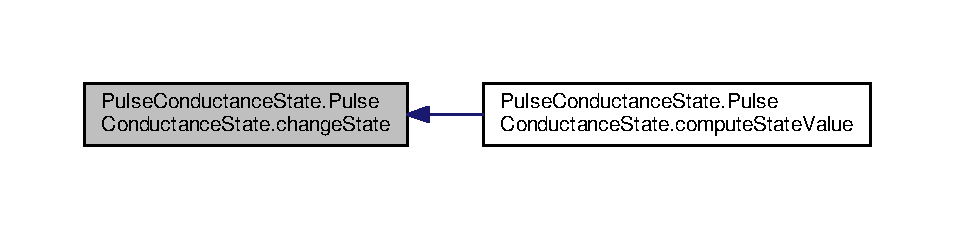
\includegraphics[width=350pt]{class_pulse_conductance_state_1_1_pulse_conductance_state_ac1ee5a9b9dc0ad6aa8e86052aa17268f_icgraph}
\end{center}
\end{figure}


\hypertarget{class_pulse_conductance_state_1_1_pulse_conductance_state_ae81d1a5bbbf4fd80db0ded06631bd9c2}{\index{Pulse\-Conductance\-State\-::\-Pulse\-Conductance\-State@{Pulse\-Conductance\-State\-::\-Pulse\-Conductance\-State}!compute\-State\-Value@{compute\-State\-Value}}
\index{compute\-State\-Value@{compute\-State\-Value}!PulseConductanceState::PulseConductanceState@{Pulse\-Conductance\-State\-::\-Pulse\-Conductance\-State}}
\subsubsection[{compute\-State\-Value}]{\setlength{\rightskip}{0pt plus 5cm}def Pulse\-Conductance\-State.\-Pulse\-Conductance\-State.\-compute\-State\-Value (
\begin{DoxyParamCaption}
\item[{}]{self, }
\item[{}]{t}
\end{DoxyParamCaption}
)}}\label{class_pulse_conductance_state_1_1_pulse_conductance_state_ae81d1a5bbbf4fd80db0ded06631bd9c2}


Compute the state value by using the approximation of Destexhe (1997) to compute the Hodgkin-\/\-Huxley states. 


\begin{DoxyItemize}
\item Input\-:
\begin{DoxyItemize}
\item {\bfseries t}\-: current instant, in ms. 
\end{DoxyItemize}
\end{DoxyItemize}

Definition at line 116 of file Pulse\-Conductance\-State.\-py.



Here is the call graph for this function\-:\nopagebreak
\begin{figure}[H]
\begin{center}
\leavevmode
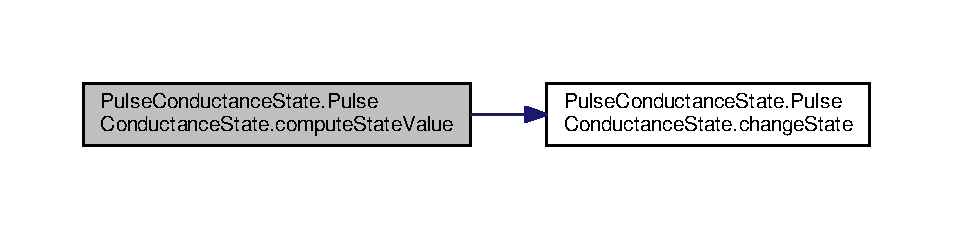
\includegraphics[width=350pt]{class_pulse_conductance_state_1_1_pulse_conductance_state_ae81d1a5bbbf4fd80db0ded06631bd9c2_cgraph}
\end{center}
\end{figure}




\subsection{Member Data Documentation}
\hypertarget{class_pulse_conductance_state_1_1_pulse_conductance_state_a0677d7b972a6f6a12abc666212a12297}{\index{Pulse\-Conductance\-State\-::\-Pulse\-Conductance\-State@{Pulse\-Conductance\-State\-::\-Pulse\-Conductance\-State}!act\-Type@{act\-Type}}
\index{act\-Type@{act\-Type}!PulseConductanceState::PulseConductanceState@{Pulse\-Conductance\-State\-::\-Pulse\-Conductance\-State}}
\subsubsection[{act\-Type}]{\setlength{\rightskip}{0pt plus 5cm}Pulse\-Conductance\-State.\-Pulse\-Conductance\-State.\-act\-Type}}\label{class_pulse_conductance_state_1_1_pulse_conductance_state_a0677d7b972a6f6a12abc666212a12297}


Definition at line 80 of file Pulse\-Conductance\-State.\-py.

\hypertarget{class_pulse_conductance_state_1_1_pulse_conductance_state_a5fe4e2c9035df43a1e8eb9d66d669e14}{\index{Pulse\-Conductance\-State\-::\-Pulse\-Conductance\-State@{Pulse\-Conductance\-State\-::\-Pulse\-Conductance\-State}!alpha\-\_\-ms1@{alpha\-\_\-ms1}}
\index{alpha\-\_\-ms1@{alpha\-\_\-ms1}!PulseConductanceState::PulseConductanceState@{Pulse\-Conductance\-State\-::\-Pulse\-Conductance\-State}}
\subsubsection[{alpha\-\_\-ms1}]{\setlength{\rightskip}{0pt plus 5cm}Pulse\-Conductance\-State.\-Pulse\-Conductance\-State.\-alpha\-\_\-ms1}}\label{class_pulse_conductance_state_1_1_pulse_conductance_state_a5fe4e2c9035df43a1e8eb9d66d669e14}


Definition at line 76 of file Pulse\-Conductance\-State.\-py.

\hypertarget{class_pulse_conductance_state_1_1_pulse_conductance_state_a8ebc0c29d97fa09699d7dfb724e94f82}{\index{Pulse\-Conductance\-State\-::\-Pulse\-Conductance\-State@{Pulse\-Conductance\-State\-::\-Pulse\-Conductance\-State}!beta\-\_\-ms1@{beta\-\_\-ms1}}
\index{beta\-\_\-ms1@{beta\-\_\-ms1}!PulseConductanceState::PulseConductanceState@{Pulse\-Conductance\-State\-::\-Pulse\-Conductance\-State}}
\subsubsection[{beta\-\_\-ms1}]{\setlength{\rightskip}{0pt plus 5cm}Pulse\-Conductance\-State.\-Pulse\-Conductance\-State.\-beta\-\_\-ms1}}\label{class_pulse_conductance_state_1_1_pulse_conductance_state_a8ebc0c29d97fa09699d7dfb724e94f82}


Definition at line 75 of file Pulse\-Conductance\-State.\-py.

\hypertarget{class_pulse_conductance_state_1_1_pulse_conductance_state_a89e0cc154bd699aee7529574a8fe556c}{\index{Pulse\-Conductance\-State\-::\-Pulse\-Conductance\-State@{Pulse\-Conductance\-State\-::\-Pulse\-Conductance\-State}!compute\-Value\-Off@{compute\-Value\-Off}}
\index{compute\-Value\-Off@{compute\-Value\-Off}!PulseConductanceState::PulseConductanceState@{Pulse\-Conductance\-State\-::\-Pulse\-Conductance\-State}}
\subsubsection[{compute\-Value\-Off}]{\setlength{\rightskip}{0pt plus 5cm}Pulse\-Conductance\-State.\-Pulse\-Conductance\-State.\-compute\-Value\-Off}}\label{class_pulse_conductance_state_1_1_pulse_conductance_state_a89e0cc154bd699aee7529574a8fe556c}


Definition at line 90 of file Pulse\-Conductance\-State.\-py.

\hypertarget{class_pulse_conductance_state_1_1_pulse_conductance_state_a7f6710b9f97ac5879888402cd5ed15d4}{\index{Pulse\-Conductance\-State\-::\-Pulse\-Conductance\-State@{Pulse\-Conductance\-State\-::\-Pulse\-Conductance\-State}!compute\-Value\-On@{compute\-Value\-On}}
\index{compute\-Value\-On@{compute\-Value\-On}!PulseConductanceState::PulseConductanceState@{Pulse\-Conductance\-State\-::\-Pulse\-Conductance\-State}}
\subsubsection[{compute\-Value\-On}]{\setlength{\rightskip}{0pt plus 5cm}Pulse\-Conductance\-State.\-Pulse\-Conductance\-State.\-compute\-Value\-On}}\label{class_pulse_conductance_state_1_1_pulse_conductance_state_a7f6710b9f97ac5879888402cd5ed15d4}


Definition at line 89 of file Pulse\-Conductance\-State.\-py.

\hypertarget{class_pulse_conductance_state_1_1_pulse_conductance_state_a53d237daaa4815ad375e2377da89845e}{\index{Pulse\-Conductance\-State\-::\-Pulse\-Conductance\-State@{Pulse\-Conductance\-State\-::\-Pulse\-Conductance\-State}!kind@{kind}}
\index{kind@{kind}!PulseConductanceState::PulseConductanceState@{Pulse\-Conductance\-State\-::\-Pulse\-Conductance\-State}}
\subsubsection[{kind}]{\setlength{\rightskip}{0pt plus 5cm}Pulse\-Conductance\-State.\-Pulse\-Conductance\-State.\-kind}}\label{class_pulse_conductance_state_1_1_pulse_conductance_state_a53d237daaa4815ad375e2377da89845e}


Definition at line 66 of file Pulse\-Conductance\-State.\-py.

\hypertarget{class_pulse_conductance_state_1_1_pulse_conductance_state_afda03b180fc3cb619de615632e725a6f}{\index{Pulse\-Conductance\-State\-::\-Pulse\-Conductance\-State@{Pulse\-Conductance\-State\-::\-Pulse\-Conductance\-State}!Pulse\-Dur\-\_\-ms@{Pulse\-Dur\-\_\-ms}}
\index{Pulse\-Dur\-\_\-ms@{Pulse\-Dur\-\_\-ms}!PulseConductanceState::PulseConductanceState@{Pulse\-Conductance\-State\-::\-Pulse\-Conductance\-State}}
\subsubsection[{Pulse\-Dur\-\_\-ms}]{\setlength{\rightskip}{0pt plus 5cm}Pulse\-Conductance\-State.\-Pulse\-Conductance\-State.\-Pulse\-Dur\-\_\-ms}}\label{class_pulse_conductance_state_1_1_pulse_conductance_state_afda03b180fc3cb619de615632e725a6f}


Definition at line 77 of file Pulse\-Conductance\-State.\-py.

\hypertarget{class_pulse_conductance_state_1_1_pulse_conductance_state_ac85aa714a187088e1b31fa2369ed4bca}{\index{Pulse\-Conductance\-State\-::\-Pulse\-Conductance\-State@{Pulse\-Conductance\-State\-::\-Pulse\-Conductance\-State}!state@{state}}
\index{state@{state}!PulseConductanceState::PulseConductanceState@{Pulse\-Conductance\-State\-::\-Pulse\-Conductance\-State}}
\subsubsection[{state}]{\setlength{\rightskip}{0pt plus 5cm}Pulse\-Conductance\-State.\-Pulse\-Conductance\-State.\-state}}\label{class_pulse_conductance_state_1_1_pulse_conductance_state_ac85aa714a187088e1b31fa2369ed4bca}


Definition at line 73 of file Pulse\-Conductance\-State.\-py.

\hypertarget{class_pulse_conductance_state_1_1_pulse_conductance_state_a55f44caf230fc3899811924118705f56}{\index{Pulse\-Conductance\-State\-::\-Pulse\-Conductance\-State@{Pulse\-Conductance\-State\-::\-Pulse\-Conductance\-State}!t0@{t0}}
\index{t0@{t0}!PulseConductanceState::PulseConductanceState@{Pulse\-Conductance\-State\-::\-Pulse\-Conductance\-State}}
\subsubsection[{t0}]{\setlength{\rightskip}{0pt plus 5cm}Pulse\-Conductance\-State.\-Pulse\-Conductance\-State.\-t0}}\label{class_pulse_conductance_state_1_1_pulse_conductance_state_a55f44caf230fc3899811924118705f56}


Definition at line 71 of file Pulse\-Conductance\-State.\-py.

\hypertarget{class_pulse_conductance_state_1_1_pulse_conductance_state_a215539a3eb60e280225053c83f386d79}{\index{Pulse\-Conductance\-State\-::\-Pulse\-Conductance\-State@{Pulse\-Conductance\-State\-::\-Pulse\-Conductance\-State}!v0@{v0}}
\index{v0@{v0}!PulseConductanceState::PulseConductanceState@{Pulse\-Conductance\-State\-::\-Pulse\-Conductance\-State}}
\subsubsection[{v0}]{\setlength{\rightskip}{0pt plus 5cm}Pulse\-Conductance\-State.\-Pulse\-Conductance\-State.\-v0}}\label{class_pulse_conductance_state_1_1_pulse_conductance_state_a215539a3eb60e280225053c83f386d79}


Definition at line 70 of file Pulse\-Conductance\-State.\-py.

\hypertarget{class_pulse_conductance_state_1_1_pulse_conductance_state_a832cdff7f315b8c16bef00642fb385dd}{\index{Pulse\-Conductance\-State\-::\-Pulse\-Conductance\-State@{Pulse\-Conductance\-State\-::\-Pulse\-Conductance\-State}!value@{value}}
\index{value@{value}!PulseConductanceState::PulseConductanceState@{Pulse\-Conductance\-State\-::\-Pulse\-Conductance\-State}}
\subsubsection[{value}]{\setlength{\rightskip}{0pt plus 5cm}Pulse\-Conductance\-State.\-Pulse\-Conductance\-State.\-value}}\label{class_pulse_conductance_state_1_1_pulse_conductance_state_a832cdff7f315b8c16bef00642fb385dd}


Definition at line 67 of file Pulse\-Conductance\-State.\-py.



The documentation for this class was generated from the following file\-:\begin{DoxyCompactItemize}
\item 
\hyperlink{_pulse_conductance_state_8py}{Pulse\-Conductance\-State.\-py}\end{DoxyCompactItemize}

\hypertarget{class_synapse_1_1_synapse}{}\section{Synapse.\+Synapse Class Reference}
\label{class_synapse_1_1_synapse}\index{Synapse.\+Synapse@{Synapse.\+Synapse}}


Implements the synapse model from Destexhe (1994) using the computational method from Lytton (1996).  


\subsection*{Public Member Functions}
\begin{DoxyCompactItemize}
\item 
def \hyperlink{class_synapse_1_1_synapse_a07d8bf346901e5db0ba72d5397057bd2}{\+\_\+\+\_\+init\+\_\+\+\_\+} (self, conf, \hyperlink{class_synapse_1_1_synapse_a133990bf3ab7f1efa8b416be73d07a11}{pool}, index, compartment, \hyperlink{class_synapse_1_1_synapse_aa2ea45450a3ad13cfefcae9fabe6ce15}{kind}, \hyperlink{class_synapse_1_1_synapse_a031af2fe7be76f9b5f69c087228a1b9a}{neuron\+Kind})
\begin{DoxyCompactList}\small\item\em Constructor. \end{DoxyCompactList}\end{DoxyCompactItemize}
\subsection*{Public Attributes}
\begin{DoxyCompactItemize}
\item 
\hyperlink{class_synapse_1_1_synapse_a133990bf3ab7f1efa8b416be73d07a11}{pool}
\item 
\hyperlink{class_synapse_1_1_synapse_aa2ea45450a3ad13cfefcae9fabe6ce15}{kind}
\item 
\hyperlink{class_synapse_1_1_synapse_a031af2fe7be76f9b5f69c087228a1b9a}{neuron\+Kind}
\item 
\hyperlink{class_synapse_1_1_synapse_adc80e9a62c17b29a92c2e7a0413e572d}{Eq\+Pot\+\_\+mV}
\item 
\hyperlink{class_synapse_1_1_synapse_ae15502cd5d5604d38328b2b1432477d7}{alpha\+\_\+ms1}
\item 
\hyperlink{class_synapse_1_1_synapse_ab59f413cbd21555531be209dee307a97}{beta\+\_\+ms1}
\item 
\hyperlink{class_synapse_1_1_synapse_ae4bcd698c5be77c2a6629d511d75f046}{Tmax\+\_\+mM}
\item 
\hyperlink{class_synapse_1_1_synapse_a09b9b092efcb0d6745fa32fadcd46375}{t\+Peak\+\_\+ms}
\begin{DoxyCompactList}\small\item\em Pulse duration, in ms. \end{DoxyCompactList}\item 
\hyperlink{class_synapse_1_1_synapse_a7922dac4765183cb6052905cc0d251cb}{gmax\+\_\+muS}
\item 
\hyperlink{class_synapse_1_1_synapse_a14adfda48133bd314f4dcd65fc9a2366}{delay\+\_\+ms}
\item 
\hyperlink{class_synapse_1_1_synapse_a67a1454de1ef2f08ffa3a10bf8466158}{dynamics}
\item 
\hyperlink{class_synapse_1_1_synapse_aa37e9a9bbac9358b50ba5280439ad319}{variation}
\item 
\hyperlink{class_synapse_1_1_synapse_a875adea3ef112a9750532b5e21d47e93}{time\+Constant\+\_\+ms}
\item 
\hyperlink{class_synapse_1_1_synapse_a470750725ecb176e048a973b9dc23ea3}{g\+Max\+Tot\+\_\+muS}
\begin{DoxyCompactList}\small\item\em The sum of individual conductances of all synapses in the compartment, in $\mu$S ( $G_{max} = \limits\sum_{i=1}^Ng_i$). \end{DoxyCompactList}\item 
\hyperlink{class_synapse_1_1_synapse_a6e55e008336cc47551669f3d77248d57}{number\+Of\+Incoming\+Synapses}
\item 
\hyperlink{class_synapse_1_1_synapse_afd263d49a97910efd8955a2aadef50e0}{r\+Inf}
\begin{DoxyCompactList}\small\item\em The fraction of postsynaptic receptors that would be bound to neurotransmitters after an infinite amount of time with neurotransmitter being released. \end{DoxyCompactList}\item 
\hyperlink{class_synapse_1_1_synapse_aae46f8edd1e94ea2ab51e3612afd3a3f}{tau\+On}
\begin{DoxyCompactList}\small\item\em Time constant during a pulse, in ms. \end{DoxyCompactList}\item 
\hyperlink{class_synapse_1_1_synapse_afd5638a223c3fdcc672002dbced7bed0}{tau\+Off}
\begin{DoxyCompactList}\small\item\em Time constant after a pulse, in ms. \end{DoxyCompactList}\item 
\hyperlink{class_synapse_1_1_synapse_aa9ae256b272ceb8e9e4a931a9cd5d163}{exp\+Finish}
\begin{DoxyCompactList}\small\item\em Is the value of the exponential at the end of the pulse. \end{DoxyCompactList}\item 
\hyperlink{class_synapse_1_1_synapse_af8779bbc2ee2c5ae7747ee5cfbcf112e}{Non}
\begin{DoxyCompactList}\small\item\em Sum of the fractions of the individual conductances that are receiving neurotransmitter (during pulse) relative to the $G_{max}$. \end{DoxyCompactList}\item 
\hyperlink{class_synapse_1_1_synapse_ae759c51a7196995510fe3eb086050c76}{Ron}
\begin{DoxyCompactList}\small\item\em Sum of the fraction of postsynaptic receptors that are bound to neurotransmitters of all the individual synapses that have neurotransmitters being released (during the pulse). \end{DoxyCompactList}\item 
\hyperlink{class_synapse_1_1_synapse_ae67ffbbd23cd9c56f20bda9e8e040663}{Roff}
\begin{DoxyCompactList}\small\item\em Sum of the fraction of postsynaptic receptors that are bound to neurotransmitters of all the individual synapses that do not have neurotransmitters being released (before and after the pulse). \end{DoxyCompactList}\item 
\hyperlink{class_synapse_1_1_synapse_ad0adf1cb832bd7ce7918f2779171d7d7}{t0}
\begin{DoxyCompactList}\small\item\em Instant that the last spike arrived to the compartment. \end{DoxyCompactList}\item 
\hyperlink{class_synapse_1_1_synapse_a89d3762daa9c60be63403a5ce9fd9a84}{conductance\+State}
\item 
\hyperlink{class_synapse_1_1_synapse_acdc426c52a2a13183d5f8c54a830bfa2}{t\+Begin\+Of\+Pulse}
\item 
\hyperlink{class_synapse_1_1_synapse_adfd02fa815d45efd0cb1bc0124fe2c90}{t\+End\+Of\+Pulse}
\item 
\hyperlink{class_synapse_1_1_synapse_a7df1cc4e7b014e7286b0bbb99079abcf}{t\+Last\+Pulse}
\item 
\hyperlink{class_synapse_1_1_synapse_adc85234a081ad18bf19473be530dcf78}{ri}
\begin{DoxyCompactList}\small\item\em List with the fractions of postsynaptic receptors that are bound to neurotransmitters of the individual synapses. \end{DoxyCompactList}\item 
\hyperlink{class_synapse_1_1_synapse_a714c95723607acad52af96ad55b6c575}{ti}
\begin{DoxyCompactList}\small\item\em List with the instants of spike arriving at each conductance, in ms. \end{DoxyCompactList}\item 
\hyperlink{class_synapse_1_1_synapse_ab987766ddedc7dc1cda9602eef6cb017}{dynamic\+Gmax}
\end{DoxyCompactItemize}


\subsection{Detailed Description}
Implements the synapse model from Destexhe (1994) using the computational method from Lytton (1996). 

Definition at line 323 of file Synapse.\+py.



\subsection{Constructor \& Destructor Documentation}
\index{Synapse\+::\+Synapse@{Synapse\+::\+Synapse}!\+\_\+\+\_\+init\+\_\+\+\_\+@{\+\_\+\+\_\+init\+\_\+\+\_\+}}
\index{\+\_\+\+\_\+init\+\_\+\+\_\+@{\+\_\+\+\_\+init\+\_\+\+\_\+}!Synapse\+::\+Synapse@{Synapse\+::\+Synapse}}
\subsubsection[{\texorpdfstring{\+\_\+\+\_\+init\+\_\+\+\_\+(self, conf, pool, index, compartment, kind, neuron\+Kind)}{__init__(self, conf, pool, index, compartment, kind, neuronKind)}}]{\setlength{\rightskip}{0pt plus 5cm}def Synapse.\+Synapse.\+\_\+\+\_\+init\+\_\+\+\_\+ (
\begin{DoxyParamCaption}
\item[{}]{self, }
\item[{}]{conf, }
\item[{}]{pool, }
\item[{}]{index, }
\item[{}]{compartment, }
\item[{}]{kind, }
\item[{}]{neuron\+Kind}
\end{DoxyParamCaption}
)}\hypertarget{class_synapse_1_1_synapse_a07d8bf346901e5db0ba72d5397057bd2}{}\label{class_synapse_1_1_synapse_a07d8bf346901e5db0ba72d5397057bd2}


Constructor. 


\begin{DoxyItemize}
\item Input\+:
\begin{DoxyItemize}
\item {\bfseries conf}\+: \hyperlink{namespace_configuration}{Configuration} object with the simulation parameters.
\item {\bfseries pool}\+: string with identification of the pool to which the synapse belongs.
\item {\bfseries index}\+: integer identification of the unit in the pool.
\item {\bfseries compartment}\+: integer identification of the compartment of the unit where the synapse is.
\item {\bfseries kind}\+: string with the type of synapse. It can be {\itshape excitatory} or {\itshape inhibitory}.
\item {\bfseries neuron\+Kind}\+: 
\end{DoxyItemize}
\end{DoxyItemize}

Definition at line 343 of file Synapse.\+py.



\subsection{Member Data Documentation}
\index{Synapse\+::\+Synapse@{Synapse\+::\+Synapse}!alpha\+\_\+ms1@{alpha\+\_\+ms1}}
\index{alpha\+\_\+ms1@{alpha\+\_\+ms1}!Synapse\+::\+Synapse@{Synapse\+::\+Synapse}}
\subsubsection[{\texorpdfstring{alpha\+\_\+ms1}{alpha_ms1}}]{\setlength{\rightskip}{0pt plus 5cm}Synapse.\+Synapse.\+alpha\+\_\+ms1}\hypertarget{class_synapse_1_1_synapse_ae15502cd5d5604d38328b2b1432477d7}{}\label{class_synapse_1_1_synapse_ae15502cd5d5604d38328b2b1432477d7}


Definition at line 349 of file Synapse.\+py.

\index{Synapse\+::\+Synapse@{Synapse\+::\+Synapse}!beta\+\_\+ms1@{beta\+\_\+ms1}}
\index{beta\+\_\+ms1@{beta\+\_\+ms1}!Synapse\+::\+Synapse@{Synapse\+::\+Synapse}}
\subsubsection[{\texorpdfstring{beta\+\_\+ms1}{beta_ms1}}]{\setlength{\rightskip}{0pt plus 5cm}Synapse.\+Synapse.\+beta\+\_\+ms1}\hypertarget{class_synapse_1_1_synapse_ab59f413cbd21555531be209dee307a97}{}\label{class_synapse_1_1_synapse_ab59f413cbd21555531be209dee307a97}


Definition at line 350 of file Synapse.\+py.

\index{Synapse\+::\+Synapse@{Synapse\+::\+Synapse}!conductance\+State@{conductance\+State}}
\index{conductance\+State@{conductance\+State}!Synapse\+::\+Synapse@{Synapse\+::\+Synapse}}
\subsubsection[{\texorpdfstring{conductance\+State}{conductanceState}}]{\setlength{\rightskip}{0pt plus 5cm}Synapse.\+Synapse.\+conductance\+State}\hypertarget{class_synapse_1_1_synapse_a89d3762daa9c60be63403a5ce9fd9a84}{}\label{class_synapse_1_1_synapse_a89d3762daa9c60be63403a5ce9fd9a84}


Definition at line 400 of file Synapse.\+py.

\index{Synapse\+::\+Synapse@{Synapse\+::\+Synapse}!delay\+\_\+ms@{delay\+\_\+ms}}
\index{delay\+\_\+ms@{delay\+\_\+ms}!Synapse\+::\+Synapse@{Synapse\+::\+Synapse}}
\subsubsection[{\texorpdfstring{delay\+\_\+ms}{delay_ms}}]{\setlength{\rightskip}{0pt plus 5cm}Synapse.\+Synapse.\+delay\+\_\+ms}\hypertarget{class_synapse_1_1_synapse_a14adfda48133bd314f4dcd65fc9a2366}{}\label{class_synapse_1_1_synapse_a14adfda48133bd314f4dcd65fc9a2366}


Definition at line 356 of file Synapse.\+py.

\index{Synapse\+::\+Synapse@{Synapse\+::\+Synapse}!dynamic\+Gmax@{dynamic\+Gmax}}
\index{dynamic\+Gmax@{dynamic\+Gmax}!Synapse\+::\+Synapse@{Synapse\+::\+Synapse}}
\subsubsection[{\texorpdfstring{dynamic\+Gmax}{dynamicGmax}}]{\setlength{\rightskip}{0pt plus 5cm}Synapse.\+Synapse.\+dynamic\+Gmax}\hypertarget{class_synapse_1_1_synapse_ab987766ddedc7dc1cda9602eef6cb017}{}\label{class_synapse_1_1_synapse_ab987766ddedc7dc1cda9602eef6cb017}


Definition at line 412 of file Synapse.\+py.

\index{Synapse\+::\+Synapse@{Synapse\+::\+Synapse}!dynamics@{dynamics}}
\index{dynamics@{dynamics}!Synapse\+::\+Synapse@{Synapse\+::\+Synapse}}
\subsubsection[{\texorpdfstring{dynamics}{dynamics}}]{\setlength{\rightskip}{0pt plus 5cm}Synapse.\+Synapse.\+dynamics}\hypertarget{class_synapse_1_1_synapse_a67a1454de1ef2f08ffa3a10bf8466158}{}\label{class_synapse_1_1_synapse_a67a1454de1ef2f08ffa3a10bf8466158}


Definition at line 357 of file Synapse.\+py.

\index{Synapse\+::\+Synapse@{Synapse\+::\+Synapse}!Eq\+Pot\+\_\+mV@{Eq\+Pot\+\_\+mV}}
\index{Eq\+Pot\+\_\+mV@{Eq\+Pot\+\_\+mV}!Synapse\+::\+Synapse@{Synapse\+::\+Synapse}}
\subsubsection[{\texorpdfstring{Eq\+Pot\+\_\+mV}{EqPot_mV}}]{\setlength{\rightskip}{0pt plus 5cm}Synapse.\+Synapse.\+Eq\+Pot\+\_\+mV}\hypertarget{class_synapse_1_1_synapse_adc80e9a62c17b29a92c2e7a0413e572d}{}\label{class_synapse_1_1_synapse_adc80e9a62c17b29a92c2e7a0413e572d}


Definition at line 348 of file Synapse.\+py.

\index{Synapse\+::\+Synapse@{Synapse\+::\+Synapse}!exp\+Finish@{exp\+Finish}}
\index{exp\+Finish@{exp\+Finish}!Synapse\+::\+Synapse@{Synapse\+::\+Synapse}}
\subsubsection[{\texorpdfstring{exp\+Finish}{expFinish}}]{\setlength{\rightskip}{0pt plus 5cm}Synapse.\+Synapse.\+exp\+Finish}\hypertarget{class_synapse_1_1_synapse_aa9ae256b272ceb8e9e4a931a9cd5d163}{}\label{class_synapse_1_1_synapse_aa9ae256b272ceb8e9e4a931a9cd5d163}


Is the value of the exponential at the end of the pulse. 

It is computed as $\exp(T_{dur}/\tau_{on})$. 

Definition at line 380 of file Synapse.\+py.

\index{Synapse\+::\+Synapse@{Synapse\+::\+Synapse}!gmax\+\_\+muS@{gmax\+\_\+muS}}
\index{gmax\+\_\+muS@{gmax\+\_\+muS}!Synapse\+::\+Synapse@{Synapse\+::\+Synapse}}
\subsubsection[{\texorpdfstring{gmax\+\_\+muS}{gmax_muS}}]{\setlength{\rightskip}{0pt plus 5cm}Synapse.\+Synapse.\+gmax\+\_\+muS}\hypertarget{class_synapse_1_1_synapse_a7922dac4765183cb6052905cc0d251cb}{}\label{class_synapse_1_1_synapse_a7922dac4765183cb6052905cc0d251cb}


Definition at line 355 of file Synapse.\+py.

\index{Synapse\+::\+Synapse@{Synapse\+::\+Synapse}!g\+Max\+Tot\+\_\+muS@{g\+Max\+Tot\+\_\+muS}}
\index{g\+Max\+Tot\+\_\+muS@{g\+Max\+Tot\+\_\+muS}!Synapse\+::\+Synapse@{Synapse\+::\+Synapse}}
\subsubsection[{\texorpdfstring{g\+Max\+Tot\+\_\+muS}{gMaxTot_muS}}]{\setlength{\rightskip}{0pt plus 5cm}Synapse.\+Synapse.\+g\+Max\+Tot\+\_\+muS}\hypertarget{class_synapse_1_1_synapse_a470750725ecb176e048a973b9dc23ea3}{}\label{class_synapse_1_1_synapse_a470750725ecb176e048a973b9dc23ea3}


The sum of individual conductances of all synapses in the compartment, in $\mu$S ( $G_{max} = \limits\sum_{i=1}^Ng_i$). 



Definition at line 363 of file Synapse.\+py.

\index{Synapse\+::\+Synapse@{Synapse\+::\+Synapse}!kind@{kind}}
\index{kind@{kind}!Synapse\+::\+Synapse@{Synapse\+::\+Synapse}}
\subsubsection[{\texorpdfstring{kind}{kind}}]{\setlength{\rightskip}{0pt plus 5cm}Synapse.\+Synapse.\+kind}\hypertarget{class_synapse_1_1_synapse_aa2ea45450a3ad13cfefcae9fabe6ce15}{}\label{class_synapse_1_1_synapse_aa2ea45450a3ad13cfefcae9fabe6ce15}


Definition at line 345 of file Synapse.\+py.

\index{Synapse\+::\+Synapse@{Synapse\+::\+Synapse}!neuron\+Kind@{neuron\+Kind}}
\index{neuron\+Kind@{neuron\+Kind}!Synapse\+::\+Synapse@{Synapse\+::\+Synapse}}
\subsubsection[{\texorpdfstring{neuron\+Kind}{neuronKind}}]{\setlength{\rightskip}{0pt plus 5cm}Synapse.\+Synapse.\+neuron\+Kind}\hypertarget{class_synapse_1_1_synapse_a031af2fe7be76f9b5f69c087228a1b9a}{}\label{class_synapse_1_1_synapse_a031af2fe7be76f9b5f69c087228a1b9a}


Definition at line 346 of file Synapse.\+py.

\index{Synapse\+::\+Synapse@{Synapse\+::\+Synapse}!Non@{Non}}
\index{Non@{Non}!Synapse\+::\+Synapse@{Synapse\+::\+Synapse}}
\subsubsection[{\texorpdfstring{Non}{Non}}]{\setlength{\rightskip}{0pt plus 5cm}Synapse.\+Synapse.\+Non}\hypertarget{class_synapse_1_1_synapse_af8779bbc2ee2c5ae7747ee5cfbcf112e}{}\label{class_synapse_1_1_synapse_af8779bbc2ee2c5ae7747ee5cfbcf112e}


Sum of the fractions of the individual conductances that are receiving neurotransmitter (during pulse) relative to the $G_{max}$. 

( 

Definition at line 387 of file Synapse.\+py.

\index{Synapse\+::\+Synapse@{Synapse\+::\+Synapse}!number\+Of\+Incoming\+Synapses@{number\+Of\+Incoming\+Synapses}}
\index{number\+Of\+Incoming\+Synapses@{number\+Of\+Incoming\+Synapses}!Synapse\+::\+Synapse@{Synapse\+::\+Synapse}}
\subsubsection[{\texorpdfstring{number\+Of\+Incoming\+Synapses}{numberOfIncomingSynapses}}]{\setlength{\rightskip}{0pt plus 5cm}Synapse.\+Synapse.\+number\+Of\+Incoming\+Synapses}\hypertarget{class_synapse_1_1_synapse_a6e55e008336cc47551669f3d77248d57}{}\label{class_synapse_1_1_synapse_a6e55e008336cc47551669f3d77248d57}


Definition at line 364 of file Synapse.\+py.

\index{Synapse\+::\+Synapse@{Synapse\+::\+Synapse}!pool@{pool}}
\index{pool@{pool}!Synapse\+::\+Synapse@{Synapse\+::\+Synapse}}
\subsubsection[{\texorpdfstring{pool}{pool}}]{\setlength{\rightskip}{0pt plus 5cm}Synapse.\+Synapse.\+pool}\hypertarget{class_synapse_1_1_synapse_a133990bf3ab7f1efa8b416be73d07a11}{}\label{class_synapse_1_1_synapse_a133990bf3ab7f1efa8b416be73d07a11}


Definition at line 344 of file Synapse.\+py.

\index{Synapse\+::\+Synapse@{Synapse\+::\+Synapse}!ri@{ri}}
\index{ri@{ri}!Synapse\+::\+Synapse@{Synapse\+::\+Synapse}}
\subsubsection[{\texorpdfstring{ri}{ri}}]{\setlength{\rightskip}{0pt plus 5cm}Synapse.\+Synapse.\+ri}\hypertarget{class_synapse_1_1_synapse_adc85234a081ad18bf19473be530dcf78}{}\label{class_synapse_1_1_synapse_adc85234a081ad18bf19473be530dcf78}


List with the fractions of postsynaptic receptors that are bound to neurotransmitters of the individual synapses. 



Definition at line 407 of file Synapse.\+py.

\index{Synapse\+::\+Synapse@{Synapse\+::\+Synapse}!r\+Inf@{r\+Inf}}
\index{r\+Inf@{r\+Inf}!Synapse\+::\+Synapse@{Synapse\+::\+Synapse}}
\subsubsection[{\texorpdfstring{r\+Inf}{rInf}}]{\setlength{\rightskip}{0pt plus 5cm}Synapse.\+Synapse.\+r\+Inf}\hypertarget{class_synapse_1_1_synapse_afd263d49a97910efd8955a2aadef50e0}{}\label{class_synapse_1_1_synapse_afd263d49a97910efd8955a2aadef50e0}


The fraction of postsynaptic receptors that would be bound to neurotransmitters after an infinite amount of time with neurotransmitter being released. 



Definition at line 370 of file Synapse.\+py.

\index{Synapse\+::\+Synapse@{Synapse\+::\+Synapse}!Roff@{Roff}}
\index{Roff@{Roff}!Synapse\+::\+Synapse@{Synapse\+::\+Synapse}}
\subsubsection[{\texorpdfstring{Roff}{Roff}}]{\setlength{\rightskip}{0pt plus 5cm}Synapse.\+Synapse.\+Roff}\hypertarget{class_synapse_1_1_synapse_ae67ffbbd23cd9c56f20bda9e8e040663}{}\label{class_synapse_1_1_synapse_ae67ffbbd23cd9c56f20bda9e8e040663}


Sum of the fraction of postsynaptic receptors that are bound to neurotransmitters of all the individual synapses that do not have neurotransmitters being released (before and after the pulse). 



Definition at line 396 of file Synapse.\+py.

\index{Synapse\+::\+Synapse@{Synapse\+::\+Synapse}!Ron@{Ron}}
\index{Ron@{Ron}!Synapse\+::\+Synapse@{Synapse\+::\+Synapse}}
\subsubsection[{\texorpdfstring{Ron}{Ron}}]{\setlength{\rightskip}{0pt plus 5cm}Synapse.\+Synapse.\+Ron}\hypertarget{class_synapse_1_1_synapse_ae759c51a7196995510fe3eb086050c76}{}\label{class_synapse_1_1_synapse_ae759c51a7196995510fe3eb086050c76}


Sum of the fraction of postsynaptic receptors that are bound to neurotransmitters of all the individual synapses that have neurotransmitters being released (during the pulse). 



Definition at line 391 of file Synapse.\+py.

\index{Synapse\+::\+Synapse@{Synapse\+::\+Synapse}!t0@{t0}}
\index{t0@{t0}!Synapse\+::\+Synapse@{Synapse\+::\+Synapse}}
\subsubsection[{\texorpdfstring{t0}{t0}}]{\setlength{\rightskip}{0pt plus 5cm}Synapse.\+Synapse.\+t0}\hypertarget{class_synapse_1_1_synapse_ad0adf1cb832bd7ce7918f2779171d7d7}{}\label{class_synapse_1_1_synapse_ad0adf1cb832bd7ce7918f2779171d7d7}


Instant that the last spike arrived to the compartment. 



Definition at line 398 of file Synapse.\+py.

\index{Synapse\+::\+Synapse@{Synapse\+::\+Synapse}!tau\+Off@{tau\+Off}}
\index{tau\+Off@{tau\+Off}!Synapse\+::\+Synapse@{Synapse\+::\+Synapse}}
\subsubsection[{\texorpdfstring{tau\+Off}{tauOff}}]{\setlength{\rightskip}{0pt plus 5cm}Synapse.\+Synapse.\+tau\+Off}\hypertarget{class_synapse_1_1_synapse_afd5638a223c3fdcc672002dbced7bed0}{}\label{class_synapse_1_1_synapse_afd5638a223c3fdcc672002dbced7bed0}


Time constant after a pulse, in ms. 

$\tau_{off}=\frac{1}{\beta}$ 

Definition at line 376 of file Synapse.\+py.

\index{Synapse\+::\+Synapse@{Synapse\+::\+Synapse}!tau\+On@{tau\+On}}
\index{tau\+On@{tau\+On}!Synapse\+::\+Synapse@{Synapse\+::\+Synapse}}
\subsubsection[{\texorpdfstring{tau\+On}{tauOn}}]{\setlength{\rightskip}{0pt plus 5cm}Synapse.\+Synapse.\+tau\+On}\hypertarget{class_synapse_1_1_synapse_aae46f8edd1e94ea2ab51e3612afd3a3f}{}\label{class_synapse_1_1_synapse_aae46f8edd1e94ea2ab51e3612afd3a3f}


Time constant during a pulse, in ms. 

$\tau_{on}=\frac{1}{\alpha.T_{max} +\beta}$ 

Definition at line 373 of file Synapse.\+py.

\index{Synapse\+::\+Synapse@{Synapse\+::\+Synapse}!t\+Begin\+Of\+Pulse@{t\+Begin\+Of\+Pulse}}
\index{t\+Begin\+Of\+Pulse@{t\+Begin\+Of\+Pulse}!Synapse\+::\+Synapse@{Synapse\+::\+Synapse}}
\subsubsection[{\texorpdfstring{t\+Begin\+Of\+Pulse}{tBeginOfPulse}}]{\setlength{\rightskip}{0pt plus 5cm}Synapse.\+Synapse.\+t\+Begin\+Of\+Pulse}\hypertarget{class_synapse_1_1_synapse_acdc426c52a2a13183d5f8c54a830bfa2}{}\label{class_synapse_1_1_synapse_acdc426c52a2a13183d5f8c54a830bfa2}


Definition at line 401 of file Synapse.\+py.

\index{Synapse\+::\+Synapse@{Synapse\+::\+Synapse}!t\+End\+Of\+Pulse@{t\+End\+Of\+Pulse}}
\index{t\+End\+Of\+Pulse@{t\+End\+Of\+Pulse}!Synapse\+::\+Synapse@{Synapse\+::\+Synapse}}
\subsubsection[{\texorpdfstring{t\+End\+Of\+Pulse}{tEndOfPulse}}]{\setlength{\rightskip}{0pt plus 5cm}Synapse.\+Synapse.\+t\+End\+Of\+Pulse}\hypertarget{class_synapse_1_1_synapse_adfd02fa815d45efd0cb1bc0124fe2c90}{}\label{class_synapse_1_1_synapse_adfd02fa815d45efd0cb1bc0124fe2c90}


Definition at line 402 of file Synapse.\+py.

\index{Synapse\+::\+Synapse@{Synapse\+::\+Synapse}!ti@{ti}}
\index{ti@{ti}!Synapse\+::\+Synapse@{Synapse\+::\+Synapse}}
\subsubsection[{\texorpdfstring{ti}{ti}}]{\setlength{\rightskip}{0pt plus 5cm}Synapse.\+Synapse.\+ti}\hypertarget{class_synapse_1_1_synapse_a714c95723607acad52af96ad55b6c575}{}\label{class_synapse_1_1_synapse_a714c95723607acad52af96ad55b6c575}


List with the instants of spike arriving at each conductance, in ms. 



Definition at line 410 of file Synapse.\+py.

\index{Synapse\+::\+Synapse@{Synapse\+::\+Synapse}!time\+Constant\+\_\+ms@{time\+Constant\+\_\+ms}}
\index{time\+Constant\+\_\+ms@{time\+Constant\+\_\+ms}!Synapse\+::\+Synapse@{Synapse\+::\+Synapse}}
\subsubsection[{\texorpdfstring{time\+Constant\+\_\+ms}{timeConstant_ms}}]{\setlength{\rightskip}{0pt plus 5cm}Synapse.\+Synapse.\+time\+Constant\+\_\+ms}\hypertarget{class_synapse_1_1_synapse_a875adea3ef112a9750532b5e21d47e93}{}\label{class_synapse_1_1_synapse_a875adea3ef112a9750532b5e21d47e93}


Definition at line 359 of file Synapse.\+py.

\index{Synapse\+::\+Synapse@{Synapse\+::\+Synapse}!t\+Last\+Pulse@{t\+Last\+Pulse}}
\index{t\+Last\+Pulse@{t\+Last\+Pulse}!Synapse\+::\+Synapse@{Synapse\+::\+Synapse}}
\subsubsection[{\texorpdfstring{t\+Last\+Pulse}{tLastPulse}}]{\setlength{\rightskip}{0pt plus 5cm}Synapse.\+Synapse.\+t\+Last\+Pulse}\hypertarget{class_synapse_1_1_synapse_a7df1cc4e7b014e7286b0bbb99079abcf}{}\label{class_synapse_1_1_synapse_a7df1cc4e7b014e7286b0bbb99079abcf}


Definition at line 403 of file Synapse.\+py.

\index{Synapse\+::\+Synapse@{Synapse\+::\+Synapse}!Tmax\+\_\+mM@{Tmax\+\_\+mM}}
\index{Tmax\+\_\+mM@{Tmax\+\_\+mM}!Synapse\+::\+Synapse@{Synapse\+::\+Synapse}}
\subsubsection[{\texorpdfstring{Tmax\+\_\+mM}{Tmax_mM}}]{\setlength{\rightskip}{0pt plus 5cm}Synapse.\+Synapse.\+Tmax\+\_\+mM}\hypertarget{class_synapse_1_1_synapse_ae4bcd698c5be77c2a6629d511d75f046}{}\label{class_synapse_1_1_synapse_ae4bcd698c5be77c2a6629d511d75f046}


Definition at line 351 of file Synapse.\+py.

\index{Synapse\+::\+Synapse@{Synapse\+::\+Synapse}!t\+Peak\+\_\+ms@{t\+Peak\+\_\+ms}}
\index{t\+Peak\+\_\+ms@{t\+Peak\+\_\+ms}!Synapse\+::\+Synapse@{Synapse\+::\+Synapse}}
\subsubsection[{\texorpdfstring{t\+Peak\+\_\+ms}{tPeak_ms}}]{\setlength{\rightskip}{0pt plus 5cm}Synapse.\+Synapse.\+t\+Peak\+\_\+ms}\hypertarget{class_synapse_1_1_synapse_a09b9b092efcb0d6745fa32fadcd46375}{}\label{class_synapse_1_1_synapse_a09b9b092efcb0d6745fa32fadcd46375}


Pulse duration, in ms. 



Definition at line 353 of file Synapse.\+py.

\index{Synapse\+::\+Synapse@{Synapse\+::\+Synapse}!variation@{variation}}
\index{variation@{variation}!Synapse\+::\+Synapse@{Synapse\+::\+Synapse}}
\subsubsection[{\texorpdfstring{variation}{variation}}]{\setlength{\rightskip}{0pt plus 5cm}Synapse.\+Synapse.\+variation}\hypertarget{class_synapse_1_1_synapse_aa37e9a9bbac9358b50ba5280439ad319}{}\label{class_synapse_1_1_synapse_aa37e9a9bbac9358b50ba5280439ad319}


Definition at line 358 of file Synapse.\+py.



The documentation for this class was generated from the following file\+:\begin{DoxyCompactItemize}
\item 
\hyperlink{_synapse_8py}{Synapse.\+py}\end{DoxyCompactItemize}

\hypertarget{class_synapses_factory_1_1_synapses_factory}{}\section{Synapses\+Factory.\+Synapses\+Factory Class Reference}
\label{class_synapses_factory_1_1_synapses_factory}\index{Synapses\+Factory.\+Synapses\+Factory@{Synapses\+Factory.\+Synapses\+Factory}}


Class to build all the synapses in the system.  


\subsection*{Public Member Functions}
\begin{DoxyCompactItemize}
\item 
def \hyperlink{class_synapses_factory_1_1_synapses_factory_a4de86ef35a3945787df975afe33733fe}{\+\_\+\+\_\+init\+\_\+\+\_\+} (self, conf, pools)
\begin{DoxyCompactList}\small\item\em Constructor. \end{DoxyCompactList}\end{DoxyCompactItemize}
\subsection*{Public Attributes}
\begin{DoxyCompactItemize}
\item 
\hyperlink{class_synapses_factory_1_1_synapses_factory_af83fbc27851417b677391ece9bf49a29}{number\+Of\+Synapses}
\begin{DoxyCompactList}\small\item\em Total number of synapses in the system. \end{DoxyCompactList}\end{DoxyCompactItemize}


\subsection{Detailed Description}
Class to build all the synapses in the system. 

Definition at line 18 of file Synapses\+Factory.\+py.



\subsection{Constructor \& Destructor Documentation}
\index{Synapses\+Factory\+::\+Synapses\+Factory@{Synapses\+Factory\+::\+Synapses\+Factory}!\+\_\+\+\_\+init\+\_\+\+\_\+@{\+\_\+\+\_\+init\+\_\+\+\_\+}}
\index{\+\_\+\+\_\+init\+\_\+\+\_\+@{\+\_\+\+\_\+init\+\_\+\+\_\+}!Synapses\+Factory\+::\+Synapses\+Factory@{Synapses\+Factory\+::\+Synapses\+Factory}}
\subsubsection[{\texorpdfstring{\+\_\+\+\_\+init\+\_\+\+\_\+(self, conf, pools)}{__init__(self, conf, pools)}}]{\setlength{\rightskip}{0pt plus 5cm}def Synapses\+Factory.\+Synapses\+Factory.\+\_\+\+\_\+init\+\_\+\+\_\+ (
\begin{DoxyParamCaption}
\item[{}]{self, }
\item[{}]{conf, }
\item[{}]{pools}
\end{DoxyParamCaption}
)}\hypertarget{class_synapses_factory_1_1_synapses_factory_a4de86ef35a3945787df975afe33733fe}{}\label{class_synapses_factory_1_1_synapses_factory_a4de86ef35a3945787df975afe33733fe}


Constructor. 


\begin{DoxyItemize}
\item Inputs\+:
\begin{DoxyItemize}
\item {\bfseries conf}\+: \hyperlink{namespace_configuration}{Configuration} object with the simulation parameters.
\item {\bfseries pools}\+: list of all the pools in the system. 
\end{DoxyItemize}
\end{DoxyItemize}

Definition at line 32 of file Synapses\+Factory.\+py.



\subsection{Member Data Documentation}
\index{Synapses\+Factory\+::\+Synapses\+Factory@{Synapses\+Factory\+::\+Synapses\+Factory}!number\+Of\+Synapses@{number\+Of\+Synapses}}
\index{number\+Of\+Synapses@{number\+Of\+Synapses}!Synapses\+Factory\+::\+Synapses\+Factory@{Synapses\+Factory\+::\+Synapses\+Factory}}
\subsubsection[{\texorpdfstring{number\+Of\+Synapses}{numberOfSynapses}}]{\setlength{\rightskip}{0pt plus 5cm}Synapses\+Factory.\+Synapses\+Factory.\+number\+Of\+Synapses}\hypertarget{class_synapses_factory_1_1_synapses_factory_af83fbc27851417b677391ece9bf49a29}{}\label{class_synapses_factory_1_1_synapses_factory_af83fbc27851417b677391ece9bf49a29}


Total number of synapses in the system. 



Definition at line 34 of file Synapses\+Factory.\+py.



The documentation for this class was generated from the following file\+:\begin{DoxyCompactItemize}
\item 
\hyperlink{_synapses_factory_8py}{Synapses\+Factory.\+py}\end{DoxyCompactItemize}

\chapter{File Documentation}
\hypertarget{_axon_delay_8py}{}\section{Axon\+Delay.\+py File Reference}
\label{_axon_delay_8py}\index{Axon\+Delay.\+py@{Axon\+Delay.\+py}}
\subsection*{Classes}
\begin{DoxyCompactItemize}
\item 
class \hyperlink{class_axon_delay_1_1_axon_delay}{Axon\+Delay.\+Axon\+Delay}
\begin{DoxyCompactList}\small\item\em Class that implements a delay correspondent to the nerve. \end{DoxyCompactList}\end{DoxyCompactItemize}
\subsection*{Namespaces}
\begin{DoxyCompactItemize}
\item 
 \hyperlink{namespace_axon_delay}{Axon\+Delay}
\end{DoxyCompactItemize}

\hypertarget{_channel_conductance_8py}{\section{Channel\-Conductance.\-py File Reference}
\label{_channel_conductance_8py}\index{Channel\-Conductance.\-py@{Channel\-Conductance.\-py}}
}
\subsection*{Classes}
\begin{DoxyCompactItemize}
\item 
class \hyperlink{class_channel_conductance_1_1_channel_conductance}{Channel\-Conductance.\-Channel\-Conductance}
\begin{DoxyCompactList}\small\item\em Class that implements a model of the ionic Channels in a compartment. \end{DoxyCompactList}\end{DoxyCompactItemize}
\subsection*{Namespaces}
\begin{DoxyCompactItemize}
\item 
\hyperlink{namespace_channel_conductance}{Channel\-Conductance}
\end{DoxyCompactItemize}

\hypertarget{_compartment_8py}{\section{Compartment.\-py File Reference}
\label{_compartment_8py}\index{Compartment.\-py@{Compartment.\-py}}
}
\subsection*{Classes}
\begin{DoxyCompactItemize}
\item 
class \hyperlink{class_compartment_1_1_compartment}{Compartment.\-Compartment}
\begin{DoxyCompactList}\small\item\em classdocs \end{DoxyCompactList}\end{DoxyCompactItemize}
\subsection*{Namespaces}
\begin{DoxyCompactItemize}
\item 
\hyperlink{namespace_compartment}{Compartment}
\end{DoxyCompactItemize}
\subsection*{Functions}
\begin{DoxyCompactItemize}
\item 
def \hyperlink{namespace_compartment_a32af1519f82a3df2abdd1a3e132cf0a8}{Compartment.\-calc\-G\-Leak}
\begin{DoxyCompactList}\small\item\em computes the leak conductance of the compartment input\-: area\-: area of the compartment in cm2 specific\-Res\-: specific resistance of the compartment in Ohm.\-cm2 output\-: g\-Leak in M\-S \end{DoxyCompactList}\end{DoxyCompactItemize}

\hypertarget{_configuration_8py}{\section{Configuration.\-py File Reference}
\label{_configuration_8py}\index{Configuration.\-py@{Configuration.\-py}}
}
\subsection*{Classes}
\begin{DoxyCompactItemize}
\item 
class \hyperlink{class_configuration_1_1_configuration}{Configuration.\-Configuration}
\begin{DoxyCompactList}\small\item\em Class that builds an object of \hyperlink{class_configuration_1_1_configuration}{Configuration}, based on a configuration file. \end{DoxyCompactList}\end{DoxyCompactItemize}
\subsection*{Namespaces}
\begin{DoxyCompactItemize}
\item 
\hyperlink{namespace_configuration}{Configuration}
\end{DoxyCompactItemize}

\hypertarget{_motor_unit_8py}{}\section{Motor\+Unit.\+py File Reference}
\label{_motor_unit_8py}\index{Motor\+Unit.\+py@{Motor\+Unit.\+py}}
\subsection*{Classes}
\begin{DoxyCompactItemize}
\item 
class \hyperlink{class_motor_unit_1_1_motor_unit}{Motor\+Unit.\+Motor\+Unit}
\begin{DoxyCompactList}\small\item\em Class that implements a motor unit model. \end{DoxyCompactList}\end{DoxyCompactItemize}
\subsection*{Namespaces}
\begin{DoxyCompactItemize}
\item 
 \hyperlink{namespace_motor_unit}{Motor\+Unit}
\end{DoxyCompactItemize}
\subsection*{Functions}
\begin{DoxyCompactItemize}
\item 
def \hyperlink{namespace_motor_unit_a5196399a48a590dfd9825f211980d2dc}{Motor\+Unit.\+calc\+G\+Coupling} (cytR, l\+Comp1, l\+Comp2, d\+Comp1, d\+Comp2)
\begin{DoxyCompactList}\small\item\em Calculates the coupling conductance between two compartments. \end{DoxyCompactList}\item 
def \hyperlink{namespace_motor_unit_a8c3fb31fb3c8c894af37c6b822d10835}{Motor\+Unit.\+comp\+G\+Coupling\+Matrix} (gc)
\begin{DoxyCompactList}\small\item\em Computes the Coupling Matrix to be used in the d\+Vdt function of the N compartments of the motor unit. \end{DoxyCompactList}\item 
def \hyperlink{namespace_motor_unit_ab7df982e859623662808361f779572f5}{Motor\+Unit.\+runge\+\_\+kutta} (derivative\+Function, t, x, time\+Step, time\+Step\+By\+Two, time\+Step\+By\+Six)
\begin{DoxyCompactList}\small\item\em Function to implement the fourth order Runge-\/\+Kutta Method to solve numerically a differential equation. \end{DoxyCompactList}\end{DoxyCompactItemize}

\hypertarget{_motor_unit_pool_8py}{\section{Motor\-Unit\-Pool.\-py File Reference}
\label{_motor_unit_pool_8py}\index{Motor\-Unit\-Pool.\-py@{Motor\-Unit\-Pool.\-py}}
}
\subsection*{Classes}
\begin{DoxyCompactItemize}
\item 
class \hyperlink{class_motor_unit_pool_1_1_motor_unit_pool}{Motor\-Unit\-Pool.\-Motor\-Unit\-Pool}
\begin{DoxyCompactList}\small\item\em Class that implements a motor unit pool. \end{DoxyCompactList}\end{DoxyCompactItemize}
\subsection*{Namespaces}
\begin{DoxyCompactItemize}
\item 
\hyperlink{namespace_motor_unit_pool}{Motor\-Unit\-Pool}
\end{DoxyCompactItemize}
\subsection*{Functions}
\begin{DoxyCompactItemize}
\item 
def \hyperlink{namespace_motor_unit_pool_a3ed1b9ccd29068fac93964327dd54bf9}{Motor\-Unit\-Pool.\-twitch\-Saturation}
\begin{DoxyCompactList}\small\item\em Computes the muscle unit force after the nonlinear saturation. \end{DoxyCompactList}\end{DoxyCompactItemize}

\hypertarget{_neural_tract_8py}{}\section{Neural\+Tract.\+py File Reference}
\label{_neural_tract_8py}\index{Neural\+Tract.\+py@{Neural\+Tract.\+py}}
\subsection*{Classes}
\begin{DoxyCompactItemize}
\item 
class \hyperlink{class_neural_tract_1_1_neural_tract}{Neural\+Tract.\+Neural\+Tract}
\begin{DoxyCompactList}\small\item\em classdocs \end{DoxyCompactList}\end{DoxyCompactItemize}
\subsection*{Namespaces}
\begin{DoxyCompactItemize}
\item 
 \hyperlink{namespace_neural_tract}{Neural\+Tract}
\end{DoxyCompactItemize}

\hypertarget{_neural_tract_unit_8py}{}\section{Neural\+Tract\+Unit.\+py File Reference}
\label{_neural_tract_unit_8py}\index{Neural\+Tract\+Unit.\+py@{Neural\+Tract\+Unit.\+py}}
\subsection*{Classes}
\begin{DoxyCompactItemize}
\item 
class \hyperlink{class_neural_tract_unit_1_1_neural_tract_unit}{Neural\+Tract\+Unit.\+Neural\+Tract\+Unit}
\begin{DoxyCompactList}\small\item\em Class that implements a neural tract unit. \end{DoxyCompactList}\end{DoxyCompactItemize}
\subsection*{Namespaces}
\begin{DoxyCompactItemize}
\item 
 \hyperlink{namespace_neural_tract_unit}{Neural\+Tract\+Unit}
\end{DoxyCompactItemize}

\hypertarget{_point_process_generator_8py}{}\section{Point\+Process\+Generator.\+py File Reference}
\label{_point_process_generator_8py}\index{Point\+Process\+Generator.\+py@{Point\+Process\+Generator.\+py}}
\subsection*{Classes}
\begin{DoxyCompactItemize}
\item 
class \hyperlink{class_point_process_generator_1_1_point_process_generator}{Point\+Process\+Generator.\+Point\+Process\+Generator}
\begin{DoxyCompactList}\small\item\em Generator of point processes. \end{DoxyCompactList}\end{DoxyCompactItemize}
\subsection*{Namespaces}
\begin{DoxyCompactItemize}
\item 
 \hyperlink{namespace_point_process_generator}{Point\+Process\+Generator}
\end{DoxyCompactItemize}
\subsection*{Functions}
\begin{DoxyCompactItemize}
\item 
def \hyperlink{namespace_point_process_generator_a01488b4f69653d1fb9653b7a8d37744e}{Point\+Process\+Generator.\+gamma\+Point} (Gamma\+Order, Gamma\+Order\+Inv)
\begin{DoxyCompactList}\small\item\em Generates a number according to a Gamma Distribution with an integer order {\bfseries Gamma\+Order}. \end{DoxyCompactList}\end{DoxyCompactItemize}

\hypertarget{_pulse_conductance_state_8py}{}\section{Pulse\+Conductance\+State.\+py File Reference}
\label{_pulse_conductance_state_8py}\index{Pulse\+Conductance\+State.\+py@{Pulse\+Conductance\+State.\+py}}
\subsection*{Classes}
\begin{DoxyCompactItemize}
\item 
class \hyperlink{class_pulse_conductance_state_1_1_pulse_conductance_state}{Pulse\+Conductance\+State.\+Pulse\+Conductance\+State}
\begin{DoxyCompactList}\small\item\em Implements the Destexhe pulse approximation of the solution of the states of the Hodgkin-\/\+Huxley neuron model. \end{DoxyCompactList}\end{DoxyCompactItemize}
\subsection*{Namespaces}
\begin{DoxyCompactItemize}
\item 
 \hyperlink{namespace_pulse_conductance_state}{Pulse\+Conductance\+State}
\end{DoxyCompactItemize}
\subsection*{Functions}
\begin{DoxyCompactItemize}
\item 
def \hyperlink{namespace_pulse_conductance_state_acfdc241fcdde637f6df3a06e426c137d}{Pulse\+Conductance\+State.\+comp\+Val\+On} (v0, alpha, beta, t, t0)
\begin{DoxyCompactList}\small\item\em Time course of the state during the pulse for the {\itshape inactivation} states and before and after the pulse for the {\itshape activation} states. \end{DoxyCompactList}\item 
def \hyperlink{namespace_pulse_conductance_state_a9c75dc1dc214912259e3aaf30203fc1c}{Pulse\+Conductance\+State.\+comp\+Val\+Off} (v0, alpha, beta, t, t0)
\begin{DoxyCompactList}\small\item\em Time course of the state during the pulse for the {\itshape activation} states and before and after the pulse for the {\itshape inactivation} states. \end{DoxyCompactList}\end{DoxyCompactItemize}

\hypertarget{simulation_8py}{}\section{simulation.\+py File Reference}
\label{simulation_8py}\index{simulation.\+py@{simulation.\+py}}
\subsection*{Namespaces}
\begin{DoxyCompactItemize}
\item 
 \hyperlink{namespacesimulation}{simulation}
\end{DoxyCompactItemize}
\subsection*{Functions}
\begin{DoxyCompactItemize}
\item 
def \hyperlink{namespacesimulation_aba125cc0d150c87088164767bbe77b81}{simulation.\+simulator} ()
\end{DoxyCompactItemize}

\hypertarget{_synapse_8py}{}\section{Synapse.\+py File Reference}
\label{_synapse_8py}\index{Synapse.\+py@{Synapse.\+py}}
\subsection*{Classes}
\begin{DoxyCompactItemize}
\item 
class \hyperlink{class_synapse_1_1_synapse}{Synapse.\+Synapse}
\begin{DoxyCompactList}\small\item\em Implements the synapse model from Destexhe (1994) using the computational method from Lytton (1996). \end{DoxyCompactList}\end{DoxyCompactItemize}
\subsection*{Namespaces}
\begin{DoxyCompactItemize}
\item 
 \hyperlink{namespace_synapse}{Synapse}
\end{DoxyCompactItemize}
\subsection*{Functions}
\begin{DoxyCompactItemize}
\item 
def \hyperlink{namespace_synapse_a400340da82be44ca7d665a8e04cd8974}{Synapse.\+comp\+Synap\+Cond} (Gmax, Ron, Roff)
\begin{DoxyCompactList}\small\item\em Computes the synaptic conductance. \end{DoxyCompactList}\item 
def \hyperlink{namespace_synapse_a685fe07b10fd8ff53778983666836dea}{Synapse.\+comp\+Ron} (Non, r\+Inf, Ron, t0, t, tau\+On)
\begin{DoxyCompactList}\small\item\em Computes the fraction of postsynaptic receptors that are bound to neurotransmitters of all the individual synapses that have neurotransmitters being released (during the pulse). \end{DoxyCompactList}\item 
def \hyperlink{namespace_synapse_a946e8e8437009fba80f7d7ead8d1eb57}{Synapse.\+comp\+Roff} (Roff, t0, t, tau\+Off)
\begin{DoxyCompactList}\small\item\em Computes the fraction of postsynaptic receptors that are bound to neurotransmitters of all the individual synapses that do not have neurotransmitters being released (before and after the pulse). \end{DoxyCompactList}\item 
def \hyperlink{namespace_synapse_a86ce19e1d63e7071f6315234ee4cb6b6}{Synapse.\+comp\+Ri\+Start} (ri, t, ti, t\+Peak, tau\+Off)
\begin{DoxyCompactList}\small\item\em Computes the fraction of bound postsynaptic receptors to neurotransmitters in individual synapses when the neurotransmitter begin (begin of the pulse). \end{DoxyCompactList}\item 
def \hyperlink{namespace_synapse_ad8ba0d5cb97f96cf8f68a75efc924488}{Synapse.\+comp\+Ri\+Stop} (r\+Inf, ri, exp\+Finish)
\begin{DoxyCompactList}\small\item\em Computes the fraction of bound postsynaptic receptors to neurotransmitters in individual synapses when the neurotransmitter release stops (the pulse ends). \end{DoxyCompactList}\item 
def \hyperlink{namespace_synapse_a15925cbb893ee12094ad1861749e3240}{Synapse.\+comp\+Ron\+Start} (Ron, ri, syn\+Contrib)
\begin{DoxyCompactList}\small\item\em Incorporates a new conductance to the set of conductances during a pulse. \end{DoxyCompactList}\item 
def \hyperlink{namespace_synapse_a695380d931b5beeed57d872bfddc423a}{Synapse.\+comp\+Roff\+Start} (Roff, ri, syn\+Contrib)
\begin{DoxyCompactList}\small\item\em Incorporates a new conductance to the set of conductances that are not during a pulse. \end{DoxyCompactList}\item 
def \hyperlink{namespace_synapse_a3fb4510e3284ad84eb4d3d8c39112a94}{Synapse.\+comp\+Ron\+Stop} (Ron, ri, syn\+Contrib)
\begin{DoxyCompactList}\small\item\em Removes a conductance from the set of conductances during a pulse. \end{DoxyCompactList}\item 
def \hyperlink{namespace_synapse_afd15218d4cf7a043cd35aa37f1593f6d}{Synapse.\+comp\+Roff\+Stop} (Roff, ri, syn\+Contrib)
\begin{DoxyCompactList}\small\item\em Removes a conductance from the set of conductances that are not during a pulse. \end{DoxyCompactList}\end{DoxyCompactItemize}

\hypertarget{_synapses_factory_8py}{\section{Synapses\-Factory.\-py File Reference}
\label{_synapses_factory_8py}\index{Synapses\-Factory.\-py@{Synapses\-Factory.\-py}}
}
\subsection*{Classes}
\begin{DoxyCompactItemize}
\item 
class \hyperlink{class_synapses_factory_1_1_synapses_factory}{Synapses\-Factory.\-Synapses\-Factory}
\begin{DoxyCompactList}\small\item\em Class to build all the synapses in the system. \end{DoxyCompactList}\end{DoxyCompactItemize}
\subsection*{Namespaces}
\begin{DoxyCompactItemize}
\item 
\hyperlink{namespace_synapses_factory}{Synapses\-Factory}
\end{DoxyCompactItemize}

%--- End generated contents ---

% Index
\backmatter
\newpage
\phantomsection
\clearemptydoublepage
\addcontentsline{toc}{chapter}{Index}
\printindex

\end{document}
